%% utexasthesis.cls is available from https://github.com/linguistics/utexas-latex
\documentclass{utexasthesis}
% \documentclass[copyright,12pt,onehalfspacing,draft]{utexasthesis}

%% Required fields
%% ===============
%% Full official title of your thesis (use \\ to force a line break)
\title{Surface Deformation Mapping and Automatic Feature Detection over the Permian Basin using InSAR}
%% Your full official name
\author{Scott Staniewicz}
%% Month and year of graduation (month may be May, August, or December)
\graduationdate{May}{2022}
%% Your thesis supervisor, full name only
\supervisor{Jingyi Ann Chen}
%% Your thesis co-supervisor, if any (leave commented if not applicable)
% \cosupervisor{Cosupervisor Name}
%% Other committee members full names, comma-separated.
%% Comment this out if empty, e.g., for a masters thesis with only a supervisor and cosupervisor.
\othercommitteemembers{Srinivas Bettadpur, Peter Hennings, Todd Humphreys, Jon Olson}

%% Optional customizations
%% =======================
%% Use Palatino as the primary font face


%\usepackage{palatino}

%https://personalinterests.lipingyang.org/options-for-appearance-of-links-in-hyperref/
% https://tex.stackexchange.com/questions/50747/options-for-appearance-of-links-in-hyperref

\usepackage{xcolor}
\hypersetup{
	colorlinks,
	linkcolor={red!50!black},
	citecolor={blue!50!black},
	urlcolor={blue!80!black}
}
% Makes all the links black, same as text
%\hypersetup{ hidelinks} 

\usepackage{amsmath}
\usepackage{amsfonts}
\usepackage{amssymb}
\usepackage{bm}

\usepackage[noend]{algpseudocode}
\usepackage{algorithm2e}
\usepackage{booktabs}
\usepackage{color}
%\usepackage{minted}
\usepackage{epsfig}
%\usepackage{apacite}
\usepackage{longtable}
\usepackage{nicematrix}
\usepackage{placeins} % FloatBarrier

\newcommand{\norm}[1]{\left\lVert#1\right\rVert}
% https://tex.stackexchange.com/questions/76273/multiple-pdfs-with-page-group-included-in-a-single-page-warning#comment977995_78020
\pdfsuppresswarningpagegroup=1



%% and Computer Modern Typewriter Proportional as the teletype font face
\renewcommand*\ttdefault{cmvtt}

\begin{document}

%% This produces the copyright page (if specified), the signature page, and title page.
\maketitle

%% The dedication is optional and fills an entire page.
\begin{dedication}


\end{dedication}

%% The acknowledgments, abstract, and table(s) of contents/tables/figures pages are numbered with roman numerals.

%% The acknowledgments is optional and fills an entire page.
\begin{acknowledgments}

\end{acknowledgments}

%% The abstract is required.
\begin{abstract}
%  The text must be either double-spaced or 1.5-spaced. Abstracts should be limited to 350 words.
% From word template: <Abstract: Should not exceed 350 words. It should be a continuous description, not disconnected notes or an outline.>

The Permian Basin has become the United States' largest producer of oil and gas over the past decade, largely due to advances in shale recovery technologies. 
Injection or withdrawal of fluids from the subsurface can induce earthquakes along existing faults, and an increased rate of low magnitude earthquakes have been observed along with the increase in hydrocarbon production in West Texas. 
%While petroleum production and wastewater injection volumes have been rising throughout the basin, the recently cataloged earthquakes are spatially clustered. 
%One significant cluster is near Pecos, TX, where increased seismic activity began in 2009 and climbed to more than 2000 earthquakes in 2017. 
To better understand the causes of these earthquakes and to assess the likelihood of infrastructure damage and safety concerns, knowledge of subsurface stress and pore pressure changes is needed. 
However, in situ measurements for characterizing the Earth’s subsurface are expensive and difficult to obtain. 
Interferometric Synthetic Aperture Radar (InSAR) is a remote sensing technique which can measure deformation of Earth's surface over broad areas with 10-100 meter spatial resolution and millimeter-to-centimeter accuracy.
These measurements can be used to derive information about Earth’s subsurface, estimate the distribution of fault slip, and infer associated seismic risk.
However, the noise sources of InSAR pose considerable challenges to achieving millimeter-level accuracy over large study areas.
%Previous InSAR induced seismicity studies have mostly focused on areas 60-by-60 km or smaller. Because InSAR tropospheric noise variance increases with the distance away from the reference point, it is difficult to expand the InSAR spatial coverage to the entire Permian basin while retaining millimeter level accuracy. 
In this thesis, we demonstrate the ability to measure subtle surface deformation features caused by petroleum production and induced earthquakes over the entire Permian Basin. 
A novel outlier detection technique is developed to detect measurements corrupted by >10 cm of turbulent tropospheric noise. 
We also present a robust time series smoothing technique for extracting nonlinear deformation in the presence of non-Gaussian noise.
%, as well as a robust 
Our deformation maps achieve basin-wide 1-3 mm/year accuracy as verified by available permanent GPS stations.
Furthermore, the recent growth in satellite data has created a need for automated and scalable algorithms for processing and interpreting large deformation maps.
%The final surface deformation products, which achieve basin-wide 1-3 mm/year accuracy, enable physics-based modeling of the subsurface processes that drive the induced seismicity. 
We develop a computer vision algorithm capable of detecting deformation features of unknown size and location in large deformation maps.
We combine this algorithm with a data-driven method for estimating tropospheric noise strength on individual SAR acquisitions to produce uncertainty measures for each automatically detected deformation feature.
The number of high-confidence detected deformation features increases substantially over the study period, which is consistent with the overall rise in oil production within the Permian Basin since 2014.


\end{abstract}

%% The table of contents is required.
\maketableofcontents

%% The following pages are numbered with arabic numerals, starting with 1


\chapter{Introduction}


\section{Problem Background}
\label{sec:chap1-problem}

%- what is the permian basin
%- why important
%- why people care about it
%- roger spent lots of time to convince why it's hard (complicated cross section structures). it's nothing to do with his work! but you show you really understand the problem and wha you're working with
%- the most important before contribution is to try to illustrate why it's a hard problem
%- not only we focused on techcnial, and work on problem that matters, but dont forget why **insar over west texas is hard**


%- first paragraph: convince it's super important problem. why perimain basin matters, and what's the problem
%- have wells, inducsed seismicity, rate hasskyrocket, mention one year has more than CA.
%- also btw, this is difficult. not all wells induce. some wells opearate fine, no issues, some wells have delayed, and keep having EQs about stop.
%- even people without background should find intersting, even without texas background.
%- people in general like to hear problems, and where people are stuck, and why they care to work on.
%- Natl academy science report shold have highlights to take.
%- ESI proposal: use from that

The Permian Basin, stretching from eastern New Mexico and covering most of West Texas (Figure \ref{fig:permian-overview}a), has become the United States' largest producer of oil and gas over the past decade. The region's production began to take off in the late 2000s, largely due to advances in horizontal drilling and multi-stage hydraulic fracturing.
Since that time, the basin also experienced an increased rate of low magnitude earthquakes \citep{Frohlich2016HistoricalReviewInduced, Atkinson2016HydraulicFracturingSeismicity, Frohlich2019OnsetCauseIncreased, Lomax2019ImprovingAbsoluteEarthquake, Savvaidis2020InducedSeismicityDelaware, Skoumal2020InducedSeismicityDelaware} (Figure \ref{fig:permian-overview}b).


Since the 1920s, researchers have recognized that injection or withdrawal of fluids from the subsurface can induce earthquakes along existing faults \citep{Council2013InducedSeismicityPotential, Simpson1988TwoTypesReservoir, Ellsworth2013InjectionInducedEarthquakes}.  Induced earthquakes near oil production and wastewater injection wells have been recently observed in the central and eastern United States in Arkansas, Ohio, Oklahoma, Texas, as well as other countries including Canada, China, and Italy \citep{Foulger2018GlobalReviewHuman}.  In Texas, despite rising volumes of production and wastewater injection throughout the Permian Basin, the recently cataloged earthquakes are spatially clustered. The vast majority of production and injection wells experience no nearby seismic activity; however, the earthquake clusters within Texas contained over 200 earthquakes of magnitude 3.0 or greater in 2021, second only to California in the contiguous United States.


\begin{figure}
	\centering
	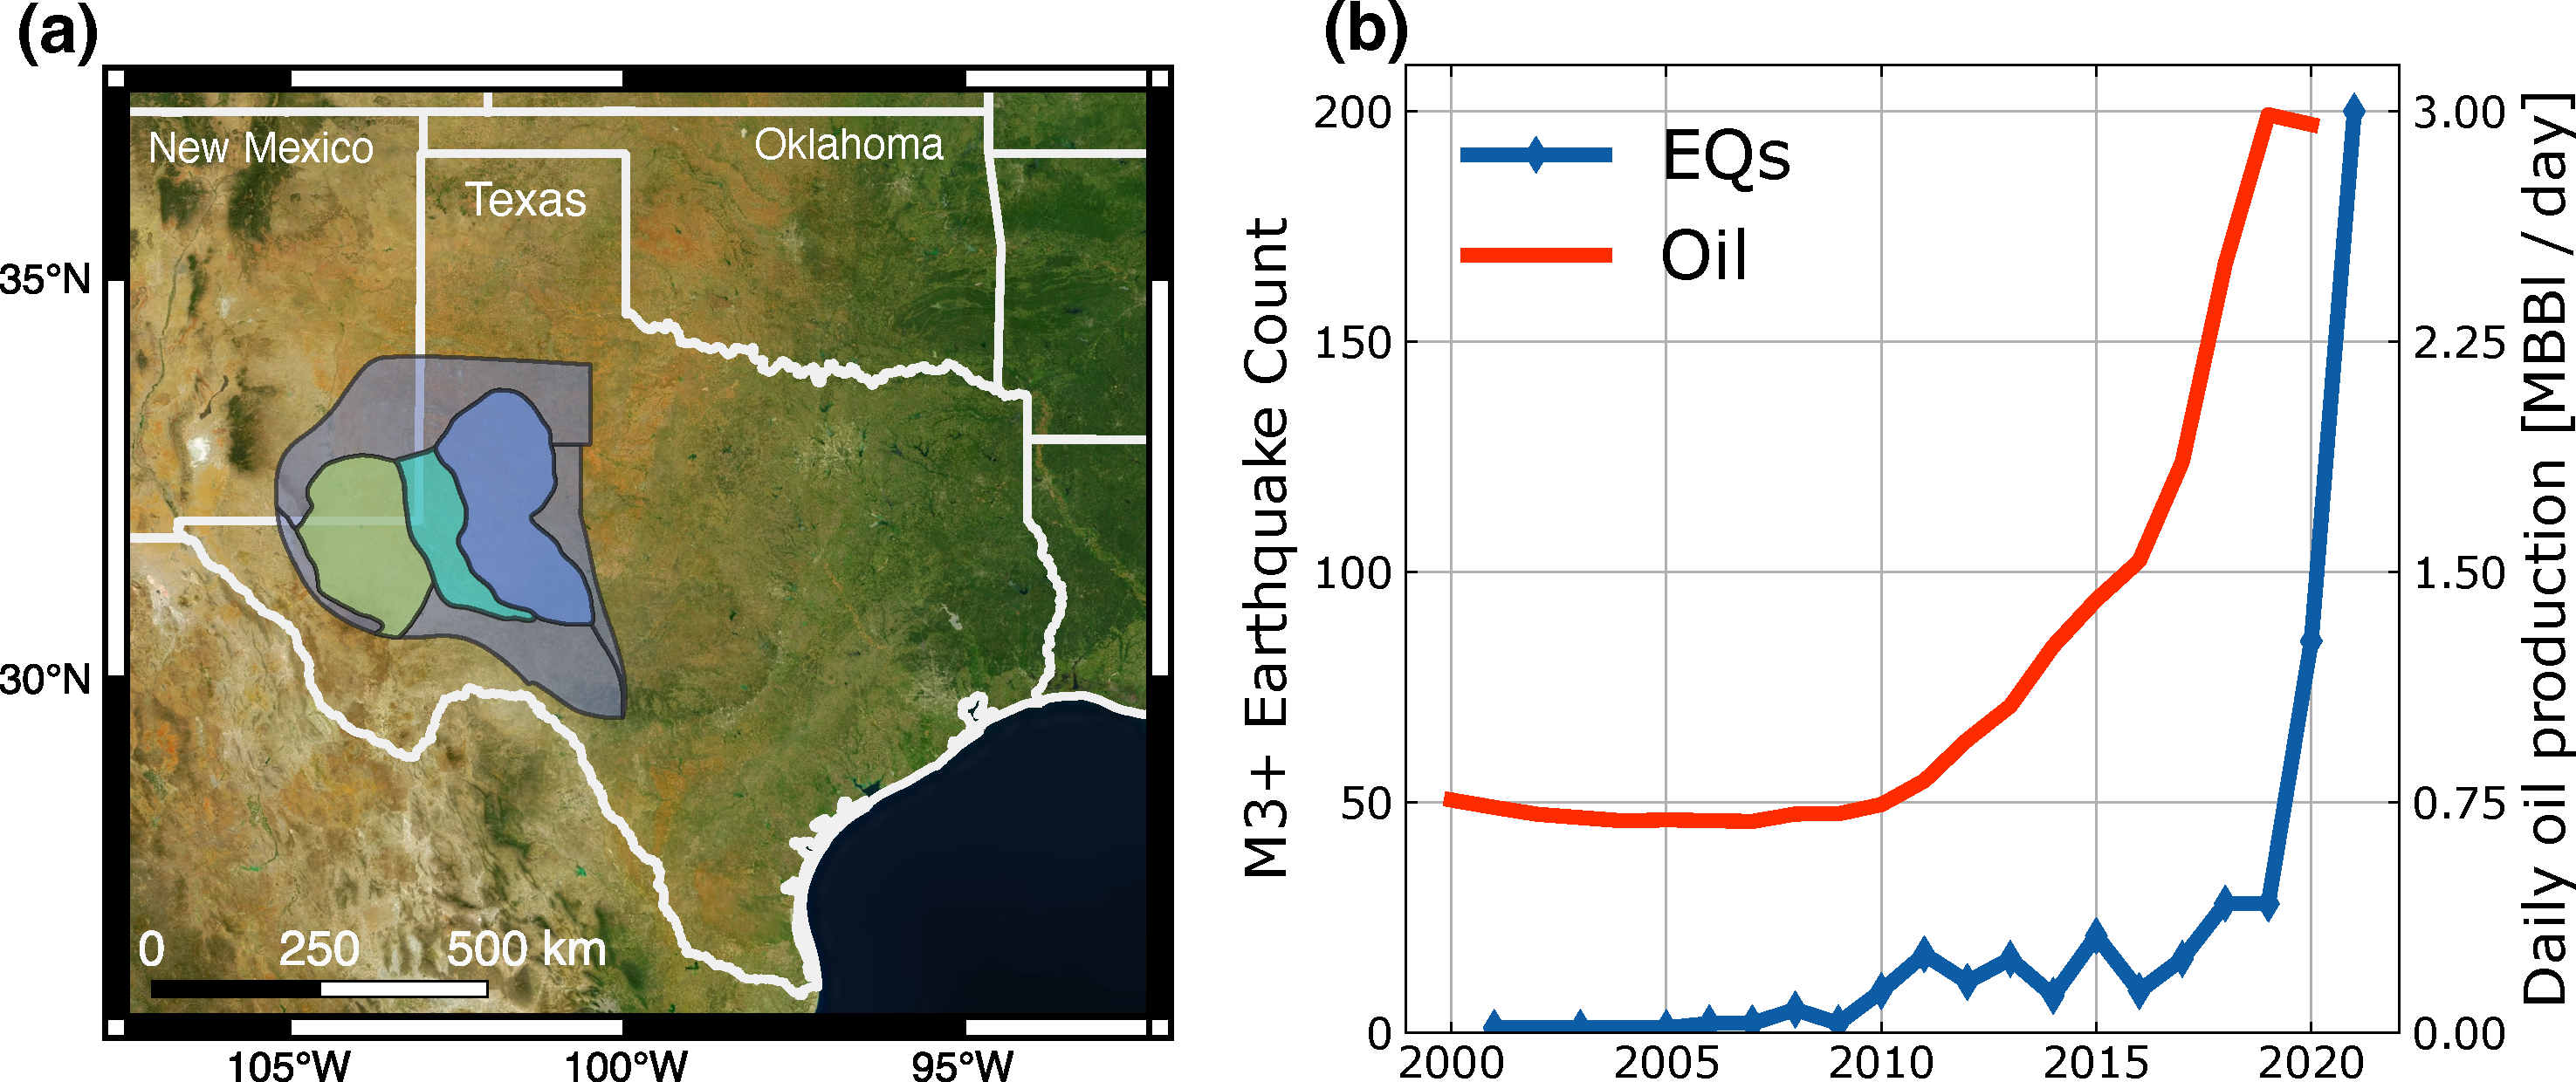
\includegraphics[width=\columnwidth]{figures/permian-overview-eqs-oil.pdf}
	\caption[Permian Basin oil production and earthquakes]{
		(a) Location of Permian Basin within Texas. The subbasins colored within the Permian Basin are (from west to east) the Delaware Basin (green), Central Basin Platform (cyan), and Midland Basin (purple).
		(b) Yearly number of magnitude 3 or larger earthquakes recorded within Texas since 2000 (blue line), and average daily oil production per year for Permian Basin wells in Texas (red line).
		Earthquakes retrieved from USGS at \url{https://earthquake.usgs.gov} . Oil Production data retrieved from the Texas Railroad Commission's production query system at \url{https://www.rrc.texas.gov} .
	}
	\label{fig:permian-overview}
\end{figure}



%One significant cluster is near Pecos, TX, where increased seismic activity began in 2009 and climbed to more than 2000 earthquakes in 2017 \citep{Frohlich2019OnsetCauseIncreased}. 

Understanding the causes of induced earthquakes be challenging, as there is limited knowledge of the locations of subsurface faults and the ways in which petroleum operations affect pore pressure \citep{Hennings2021StabilityFaultSystems}. Additionally, the Permian Basin contains many possible mechanisms which can trigger earthquakes, including oil and gas production, wastewater injection, hydraulic fracturing, and groundwater withdrawal, all operating in a geologically-complex region \citep{Smye2021VariationsVerticalStress}.
Although detailed measurement of the subsurface is infeasible across the $\sim$200,000 km$^2$ Permian Basin, the spaceborne remote sensing technique known as Interferometric Synthetic Aperture Radar (InSAR) can measure deformation of Earth's surface over wide areas with millimeter-to-centimeter accuracy \citep{Massonnet1993DisplacementFieldLanders, Buergmann2000SyntheticApertureRadar}. These surface deformation measurements can be used to derive information about Earth's subsurface, locate previously unknown faults, estimate the distribution of fault slip, and infer associated seismic risk \citep{Segall2010EarthquakeVolcanoDeformation, Elliott2016RoleSpaceBased, Huang2017FaultGeometryInversion}.

Previous InSAR studies over West Texas demonstrated the use of InSAR surface deformation data for understanding causes of induced seismicity.
For example, \cite{Kim2018AssociationLocalizedGeohazards} detected multiple deformation bowls within the Delaware Basin related to wastewater injection, $CO_2$ injection, and hydrocarbon production using Sentinel-1 InSAR data. \cite{Deng2020SurfaceDeformationInduced} used ascending Sentinel-1 LOS measurements to infer pore pressure change and Coulomb failure stress change at three sites in the southern Delaware Basin. 
However, these studies only focused on study areas $ \sim $ 60$ \times $60km or smaller. Since InSAR noise becomes more severe as the area of interest expands, it is difficult to cover to the entire Permian basin while retaining millimeter level accuracy. 

Additionally, the volume of available InSAR data has grown exponentially since the launch of Sentinel-1 in 2014. This expansion has prompted the need to develop automated methods of detecting deformation sources in large surface deformation maps.
Previous studies have applied computer vision and machine learning techniques for automated detection \citep{Anantrasirichai2018ApplicationMachineLearning, RouetLeduc2021AutonomousExtractionMillimeter, Ebmeier2016ApplicationIndependentComponent}; however, residual InSAR noise can often visually be mistaken for real deformation.
While auxiliary data sources can be used to quantify uncertainty in deformation maps \citep{Barnhart2013CharacterizingEstimatingNoise, Parker2015SystematicAssessmentAtmospheric}, these measurements typically do not have sufficient resolution to capture the kilometer-scale noise which regularly appears in West Texas data due to summer weather patterns.

%Since uncertainty quantification based on auxiliary measurements typically do not have sufficient resolution 
%the associated uncertainty quantification has usually been derived from auxiliary data sources. Since these data sources typically do not have sufficient spatial resolution to capture spatially coherent noise, 




%However, InSAR measurements contain many noise sources which pose serious challenges for attempts at routine processing over large areas.
%Specifically, errors from atmospheric noise can be over 10x as large as the deformation signals of interest.
%While InSAR has the possibility of providing a key observable for basin-scale studies on induced seismicity and its mitigation, it is necessary to mitigate the severe noise and provide detailed uncertainty measures to stakeholders.


%%%%%%%%%%%%%%%%%%%%%%%%
%Within Texas, \cite{Shirzaei2016SurfaceUpliftTime} reported indications of surface uplift due to wastewater injection near a 2012 M4.8 earthquake, though limited validation for the ALOS data was available at this site near Timpson, TX \citep{Semple2017IncompleteInventorySuspected}. \cite{Kim2018AssociationLocalizedGeohazards} detected multiple deformation bowls within the Delaware Basin related to wastewater injection, $CO_2$ injection, and hydrocarbon production using Sentinel-1 InSAR data. \cite{Zheng2019WastewaterLeakageWest} incorporated InSAR-derived surface deformation data into a poroelastic model to analyze the geomechanical processes near an uplift signal in northern West Texas. They discovered that the observed surface deformation was likely caused by injection well leakages, rather than pressure increases at the planned injection depth, and the leaks may have contributed to freshwater contamination. More recently, \cite{Deng2020SurfaceDeformationInduced} used ascending Sentinel-1 LOS measurements to infer pore pressure change and Coulomb failure stress change at three sites in the southern Delaware Basin. They suggested that certain groups of earthquakes are likely induced by fluid injection, but noted that local rock structure and media properties are key controls on the area's susceptibility to induced seismicity.

%Previous InSAR studies demonstrated the use of InSAR surface deformation data for understanding causes of induced seismicity; however, these studies only focused on study areas $ \sim $ 60-by-60km or smaller, and basin-wide InSAR surface deformation data with detailed uncertainty quantification are needed for assessing the likelihood of induced seismicity risk. Since InSAR tropospheric noise variance increases with the distance away from the reference point \citep{Emardson2003NeutralAtmosphericDelay}, it is difficult to expand the InSAR spatial coverage to the entire Permian basin while retaining millimeter level accuracy. 

%%%%%%%%%% TGRS %%%%%%%%%%%%
%Interferometric Synthetic Aperture Radar (InSAR) has made it possible to monitor surface deformation with 10s–100s meter spatial resolution and millimeter-to-centimeter accuracy (e.g. \citep{Pritchard2004InSARbasedsurvey,  Chaussard2014PredictabilityHydraulicHead,  Chen20142010SlowSlip, Biggs2017GlobalVolcanoMonitoring, Chen2016ConfinedAquiferHead, Fielding2017SurfaceDeformationNorth, Chen2019TriggeringMw7.2}). Since the launch of the Sentinel-1 mission in 2014, the quantity and quality of open-access InSAR data has grown exponentially. Processing and interpreting such data often requires artificial intelligence and computer vision algorithms without extensive manual inspection. However, designing robust and scalable computer vision algorithms for automatic detection of InSAR surface deformation features is challenging. This is because InSAR measurement noise varies substantially in both space and time, and its magnitude is often comparable or larger than subtle deformation signals of interest. In particular, residual troposphere noise in InSAR surface deformation maps are spatially coherent, and it can often be visually mistaken as real surface deformation.


%To address these challenges, previous studies developed algorithms for detecting deformation signals in pixel-wise InSAR deformation time series based on certain magnitude thresholds. The thresholds can be set manually \citep{Raspini2018ContinuousSemiAutomatic}, set using pixel-wise standard deviations \citep{Bekaert2020InsarBasedDetection}, derived from auxiliary data sources (e.g. global atmospheric weather models \citep{Parker2015SystematicAssessmentAtmospheric}, MODIS water vapor measurements \citep{Barnhart2013CharacterizingEstimatingNoise}), or derived from simulated noise parameters \citep{Havazli2021DetectionThresholdEstimates}. Principal component analysis (PCA) and independent component analysis (ICA) have also been used to explore decompositions of noisy time series data \citep{Chaussard2014PredictabilityHydraulicHead, Ebmeier2016ApplicationIndependentComponent, Gaddes2018BlindSignalSeparation}. Moreover, deep learning methods using convolutional neural networks (CNNs) have been applied to detect deformation features in individual interferograms \citep{Anantrasirichai2018ApplicationMachineLearning, Anantrasirichai2019ApplicationConvolutionalNeural} or InSAR time series \citep{RouetLeduc2021AutonomousExtractionMillimeter}. Because the detection problems are posed as a supervised learning task, they require either labeled training data \citep{Anantrasirichai2018ApplicationMachineLearning} or ground truth examples from simulated noise and deformation models \citep{Anantrasirichai2019DeepLearningApproach, RouetLeduc2021AutonomousExtractionMillimeter}. These supervised learning approaches work well when deformation signals of interest show spatial signatures that are distinct from InSAR measurement noise. In many applications, both deformation signals and tropospheric turbulence noise are spatially coherent ``blob-like'' features that look similar to human eyes.

%Automatic detection algorithms need to quantify the detection uncertainty based on the noise magnitude of a particular radar dataset. Auxiliary tropospheric data sources such as MODIS or weather models typically do not have sufficient spatial resolution to capture localized tropospheric turbulence noise at sub-kilometer scale. Here we present


\section{Contributions}
\label{sec:chap1-contributions}


The contributions of this thesis center around designing scalable methods to produce reliable surface deformation maps over large regions. We have focused on the mitigation of strong atmospheric noise and the creation of uncertainty measures which are easy to interpret for non-expert stakeholders.


The contributions may be summarized as follows:

\begin{enumerate}
	
	\item We developed Python-based InSAR time series analysis software to ingest geocoded SAR images, extract surface deformation, decompose multiple geometries into horizontal and vertical deformation, and verify results with permanent GPS stations.
	
	\item We performed a rigorous uncertainty analysis to identify the dominant noise source in the Permian Basin for Sentinel-1.  In the process, we developed a method to estimate the tropospheric noise and its power spectral density from InSAR data.
	
	\item We designed scalable, robust time series algorithms for tracking yearly changes of deformation over large regions.
	
	\item We created millimeter-level accurate maps of cumulative surface deformation that are available online for analysis. These maps contain many subsidence and uplift features near oil and gas production, as well as linear patterns near clusters of seismic activity.
	
	\item We created a computer vision algorithm to automatically detect surface deformation signals of unknown sizes in large InSAR maps. The detection algorithm produces uncertainty estimates for each visual feature in the InSAR data.
	
	
	
\end{enumerate}


\section{Thesis Roadmap}
\label{sec:chap1-roadmap}


In Chapter \ref{CHAP:2}, we introduce the principles of InSAR. We start with a review of synthetic aperture radar (SAR) image formation. We show how the phase difference between two SAR images acquired at different times can be used to infer topography or surface deformation. We outline common InSAR noise sources, emphasizing the origins of tropospheric noise, and we show how to combine many interferograms to solve for a time series of surface deformation. Finally, we show how the use of geocoded single-look complex (SLC) products enables a simple InSAR processing workflow. 


In Chapter \ref{CHAP:3}, we introduce the scientific background of the induced seismicity problem. We review the oil and gas production boom of the last decade within the Permian Basin, as well as previous studies on the increase in low magnitude earthquakes during this time. We describe the geodetic datasets available to study the problem, and we present the case to use InSAR to better inform efforts to mitigate induced seismicity.
%for new high-quality observational datasets 


In Chapter \ref{CHAP:4-GRL}, we present a simple yet effective time series method for creating cumulative surface deformation maps over large regions with severe tropospheric noise. We use the method to create yearly line-of-sight and eastward/vertical deformation maps over the oil-producing region of the Permian Basin. The method incorporates an automated outlier detection and removal algorithm, which enabled ~2 mm/year agreement with GPS measurements in the presence of $\sim$15 cm of tropospheric noise.
%we describe how to decompose deformation from multiple satellite geometries into horizontal and vertical components.


In Chapter \ref{CHAP:5-robust-ts}, we expand our robust time series methods to account for non-linear deformation. We introduce a method to extract nonlinear deformation over long time series using non-parametric LOWESS smoothing. We demonstrate the method's ability to mitigate strong tropospheric noise on synthetic data. We use the method on Sentinel-1 data to create yearly cumulative and differential surface deformation maps for 2015-2021 over the Permian Basin, where a variety of anthropogenic causes have led to local and large-scale deformation patterns.


In Chapter \ref{CHAP:6-blob}, we demonstrate methods for automatically detecting surface deformation signals in InSAR maps. We present a computer vision algorithm based on Laplacian of Gaussian filters. We show how the tropospheric noise levels can be estimated from InSAR data, and we use these estimates to simulate new instances of noise. We create confidence measures based on the simulations for automatically detected signals in real InSAR maps.


Finally, we conclude in Chapter \ref{CHAP:7} with a summary and discussions of possible directions of future research.



\chapter{Radar Interferometry Background}
\label{CHAP:2}

%In this chapter...

%Simons: operating at microwave frequencies, synthetic aperture radar (SAR) systems provide unique images representing the electrical and geometrical proper- ties of a surface in nearly all weather conditions. Since they provide their own illumination, SARs can image in daylight or at night. 

%https://www.usgs.gov/observatories/yvo/news/insar-magic-deformation-camera-no-one-saw-coming
%Tracking radars "ping" a target, record the reflected signal, and measure (1) how long it took for the ping's round trip, and (2) the frequency of the return signal. The travel time is a measure of distance to the target. The target's velocity can be determined from the frequency of the return signal, which differs from that of the transmitted signal as a result of the Doppler effect (this is the effect that makes a siren sound different when it is coming toward you versus moving away from you, for example). Air traffic control radars and police speed detectors work on this principle.

\section{Radar Imaging}
\label{sec:ch2-radar}

``Radar'' was originally an acronym for ``RAdio Detection And Ranging'' but it has since become ubiquitous enough enter the common vernacular. Unlike passive sensors that rely on illumination for outside sources, such as optical cameras, a radar is an active sensor that emits its own electromagnetic energy.  As such, radars are able to operate both day and night, and generally operate at microwave frequencies that are not blocked by clouds (between $\sim$ 1 GHz and 300 GHz, or wavelengths of 3 m to 1 mm).
%The ability to operate both day and night is one of the main advantages of radar.

The original radars developed during World War 2 were for tracking the position of targets. In these systems, the range to the target is calculated from the round trip travel time of an electromagnetic pulse that is reflected off the target, and the angle is determined by the antenna pointing direction. Later researchers developed imaging radar systems converted a series of radar pulses on a moving platform into a two-dimension image. Although these images originally had coarse resolution, research led by Carl Wiley at Goodyear in the 1950s resulted in the development of the radar imaging technique known as synthetic aperture radar (SAR) \citep{Wiley1954PulsedDopplerRadar, Wiley1985SyntheticApertureRadars}. The first demonstration of a spaceborne earth-observing SAR mission with interferometric capability was Seasat, launched by NASA in 1978 \citep{Born1979SeasatMissionOverview, Gabriel1989MappingSmallElevation}. Since that time, there have been dozens of mission launched by various space agencies, leading some to call the last decade ``the golden age of SAR'' \citep{Moreira2014GoldenAgeSpaceborne}.

%Synthetic aperture radar (SAR) is a powerful radar imaging technique which works day and night through all weather conditions.



\subsection{Timeline of SAR Constellations}
\label{sec:ch2-history}


\begin{figure}
	\centering
	\includegraphics[width=1.1\textwidth]{figures/chapter2-sar/sar-missions.pdf}
	\caption[Timeline of government SAR missions]{Timeline of government-sponsored SAR missions since 1990. Bar lengths indicate life span of mission. Bars which intersect the right edge indicate ongoing missions.
		Colors indicate the space agency operating the mission.
		Missions which provide data free of charge to the general public (as of May 2022) are marked with blue stars.
		Vertical sections of the timeline are divided by the radar frequency of the sensor, showing (from top to bottom) the X-band, C-band, and L-band missions.
		Note that SIR-C/X-SAR and SRTM were equipped with both C- and X-band sensors.	
%The acronyms for space agency operators or commercial owners are given in the legends. ASI, Agenzia Spaziale Italiana (Italian Space Agency); CNES, centre national d'etudes spatiales (France - National Centre for Space Studies); CONAE, Comisión Nacional de Actividades Espaciales (Argentina - National Space Activities Commission); CSA, Canadian Space Agency; DLR, Deutsches Zentrum fur Luft- und Raumfahrt (German Aerospace Centre); ESA, European Space Agency; INTA, Instituto Nacional de Técnica Aeroespacial (Spain - National Institute of Aerospace Technology); KARI, Korean Aerospace Research Institute; JAXA, Japan Aerospace Exploration Agency; NASA, National Aeronautics & Space Administration (USA).
}
	\label{fig:ch2-sar-missions}
\end{figure}


Figure \ref{fig:ch2-sar-missions} shows a timeline of SAR missions that have been launched by governments and space agencies since 1990. The missions are grouped vertically into the three most commonly used frequency bands for SAR sensors in earth-observing missions: L-band (wavelengths of $\sim$24 cm), C-band ($\sim$6 cm cm) and X-band ($\sim$3 cm).
During the 90s, the European Space Agency (ESA) launched two C-band SAR satellites: ERS-1 in 1991 and ERS-2 in 1995. The ERS-1 satellite provided the first practical demonstration of spaceborne InSAR's ability to capture surface deformation
when \cite{Massonnet1993DisplacementFieldLanders} mapped the surface deformation pattern caused by the 1992 Landers, California earthquake. The first L-band SAR satellite, JERS-1, was launched by NASDA\footnote{Although JERS-1 is labeled as a JAXA mission in Figure \ref{fig:ch2-sar-missions}, it was run by NASDA at the time. In 2003, NASDA merged with two other Japanese space agencies, ISAS and NAL, to form JAXA.} in 1992, and the Canadian Space Agency (CSA) launched their own C-band mission, RADARSAT-1, in 1995. In 2000, NASA flew the 11-day Shuttle Radar Topography Mission (SRTM) to generate the first high-resolution near-global topographical map of Earth \citep{Farr2007ShuttleRadarTopography}.

The most influential recent SAR mission within the science community has been Sentinel-1 \citep{Torres2012GmesSentinel1}. First launched in 2014, the Sentinel-1 satellites acquire data using the TOPSAR imaging mode which images very wide swaths ($\sim$240 km in the interferometry mode) \cite{Zan2006TopsarTerrainObservation}, allowing them revisit any point on Earth every 12 days.  Additionally, Sentinel is the first mission of its kind to provide free public data. This advanced SAR and InSAR from being an opportunistic study tool to  a operational technique to monitor nearly anywhere on Earth  \cite{Rosen2021ShiftingGround}. Sentinel-1 is currently the only active mission providing open SAR data; however, the future NISAR ISRO SAR mission (NISAR) will also provide free L-band SAR data with global coverage \citep{Rosen2015NasaIsroSar}.


\begin{figure}
	\centering
	\includegraphics[width=1.0\textwidth]{figures/chapter2-sar/sar-private-constellations.pdf}
	\caption[Private sector SAR constellations]{SAR constellations run by private companies, showing the number of currently launched satellites (blue) stacked under the number of future planned launches (gold). Note the broken y-axis scale, as two companies 
		%	(China Electronics Technology Group and PredaSAR) 
		are planning constellations of 96 satellites.
	}
	\label{fig:ch2-sar-private-const}
\end{figure}



The first small SAR SmallSats (satellites weighing under 180 kg) have been launched by private companies over the past four years (Figure \ref{fig:ch2-sar-private-const}). Finland's ICEYE had its first succesful launch in January 2018, while Capella Space had their first launch 11 months later. Seven other companies have since launched at least 1 SAR satellite, and in the next five years, there are plans to launch over 500 additional SAR SmallSats \citep{Kulu2021SatelliteConstellations2021}. While many large SAR constellations expect sub-hourly revisit time for any given point on earth \citep{Stringham2019CapellaXband}, only the large government SAR missions, such as Sentinel-1, ALOS, and NISAR, explicitly plan for consistent global coverage in their mission objectives. However, the possibility of daily or hourly InSAR revisit times opens many new applications previously not possible with the 6-12 day revisit times of large SAR missions \citep{YagueMartinez2021TowardsFrequentFlood, Taylor2021RemoteSensingMountain, Kitajima2021PotentialSarSmall}.




\section{Synthetic Aperture Radar}
\label{sec:ch2-sar}


Synthetic aperture radar is an imaging technique that uses a radar mounted on a moving platform. A two-dimensional image is created by coherently processing the returned energy from transmitted pulses. While the images are often displayed in grayscale and may appear similar to optical images, they represent the electrical and geometrical properties of the objects in the scene \cite{Simons2007InterferometricSyntheticAperture}.
%To create a radar image, the energy scattered by points on the ground must be collected and focused in two dimensions.  The image represents the electrical and geometrical properties of the scene \cite{Simons2007InterferometricSyntheticAperture} 


The SAR imaging geometry is shown in Figure \ref{fig:ch2-sar-geometry}. A side-looking radar with look angle $\theta$ moves in the azimuth directory and repeatedly emits pulses at some interval (called the \emph{pulse repetition interval}, or PRI) which travel in the range direction.
%The illuminated portion of the ground has a swath width of $r \lambda / w$
%The width of the swath for stripmap operation is controlled by the antenna width, $w$, as $r \lambda / w$. Likewise, the size of the illuminated swath in the along track direction is $r \lambda / L$.
The line of sight (LOS) vector is defined as the unit vector pointing from the radar antenna to a point in the illuminated swath.
Each pulse illuminates a portion of the ground known as the radar footprint.


\begin{figure}
	\centering
		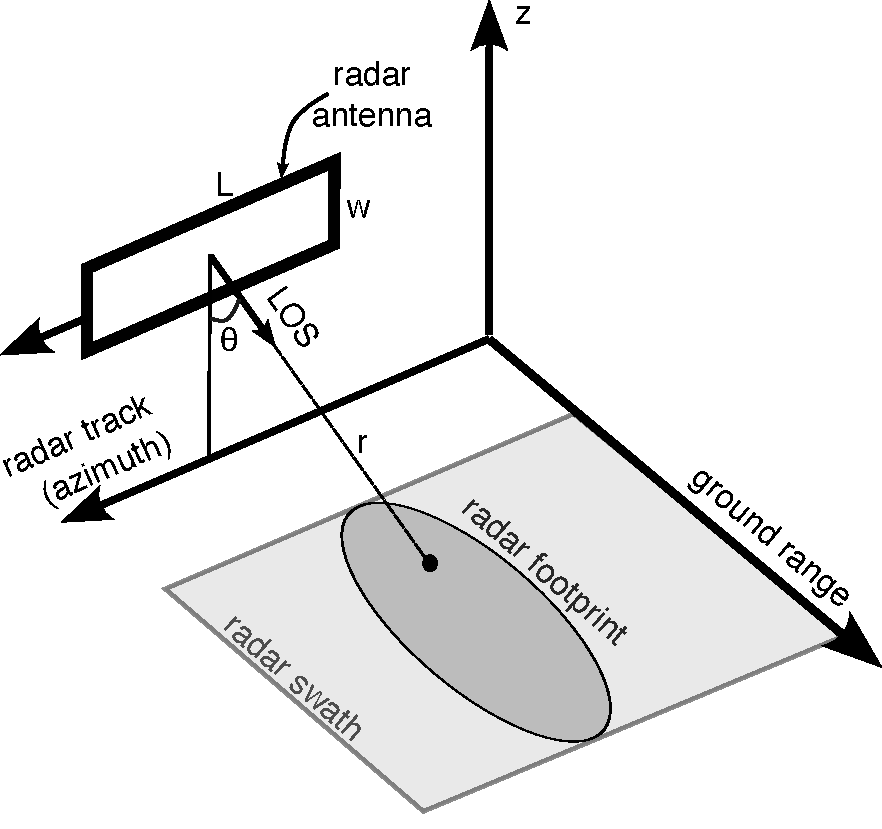
\includegraphics[width=0.99\linewidth]{figures/chapter2-sar/sar-geometry.pdf}
	\caption[Acquisition geometry of a SAR platform]{
	A platform moving in the azimuth/along-track direction contains a radar instrument with look angle $\theta$.    The slant range $r$ to the ground point is measured along the line-of-sight (LOS) direction from the antenna to the ground.
   	The radar antenna shown has length $L$ (in the azimuth direction) and width $w$.
   	As the radar sends out pulses, each one illuminates into an area on the ground called the beam ``footprint'' (oval shape). 
%   	As the platform moves and sends more pulses, they sweep out the radar swath (gray region).
	}
	\label{fig:ch2-sar-geometry}
\end{figure}

% Resolution: shorter pulse better resolution, but also lowers SNR. To get around tradeoff, send long with LFM chip to high snr and fine resolution in range direction


The signal-to-noise ratio (SNR) of the system depends on the total energy transmitted.  SNR can be increased by either sending a higher peak power (which is often limited by design constraints) or sending pulses with longer duration $\tau$. This choice creates a dilemma: in the absence further processing, sending pulses with a larger $\tau$ results in coarser range resolution $\delta_r$, where resolution is the ability to distinguish points illuminated by the same radar pulse. The illuminated size in range is $\delta_r = \frac{c \tau}{2}$, where $c \approx 3 \times 10^8$ is the speed of light. Thus, a pulse with $\tau = 30 $ microseconds would have a resolution of approximately 4.5 km. 

For this reason, SAR systems usually transmit pulsed waveforms called \emph{chirps} whose frequency $f$ increases or decreases over time. For example, in a linear frequency moduled (LFM) chirp, the frequency can be written as $ f(t) = k t$, where $k$ is the chirp slope (in Hz / s) and $-\tau / 2 < t < \tau/2$.
These special waveforms allow the receiver to correlate the returned echoes with a \emph{matched filter}, or a replica of the transmitted chirp. The improved range resolution depends on the frequency bandwidth of the chirp: $BW = f_{max} - f_{min}$.
For a given $BW$, the range resolution can be written as $\delta_r = \frac{c}{2 BW}$. 
%which means the resolution improves by a factor of $\tau \cdot BW$ (known as the \emph{time-bandwidth product}).


Figure \ref{fig:ch2-range-compress} demonstrates the effect of using a chirp waveform on range resolution. An example chirp with parameters matching the ERS-1 satellite (Figure \ref{fig:ch2-range-compress}a)
%The real part of an example chirp with parameters matching the ERS-1 satellite has an oscillation frequency which increases linearly over time (Figure \ref{fig:ch2-range-compress}a). 
has a duration of $\tau \approx 37.12 \mu s$ and chirp slope $k = 4 \times 10^{11} Hz / s$, resulting in frequency bandwidth $BW = k \tau$ $\approx$15.5 MHz (Figure \ref{fig:ch2-range-compress}b). By convolving the transmitted chirp with its complex conjugate, we get the impulse response of a point scatterer (Figure \ref{fig:ch2-range-compress}c). If a chirp with the same time duration had a smaller slope $k$ (Figure \ref{fig:ch2-range-compress}d), the bandwidth would shrink by the same proportion (Figure \ref{fig:ch2-range-compress}e), and the impulse response would also have worse resolution (Figure \ref{fig:ch2-range-compress}f).
Thus, we see that using chirped waveforms eliminates the original problem, as a pulse with larger bandwidth actually has a better resolution than a shorter pulse.


\begin{figure}
	\centering
%	\includegraphics[width=0.99\linewidth]{figures/chapter2-sar/range-compress.pdf}
	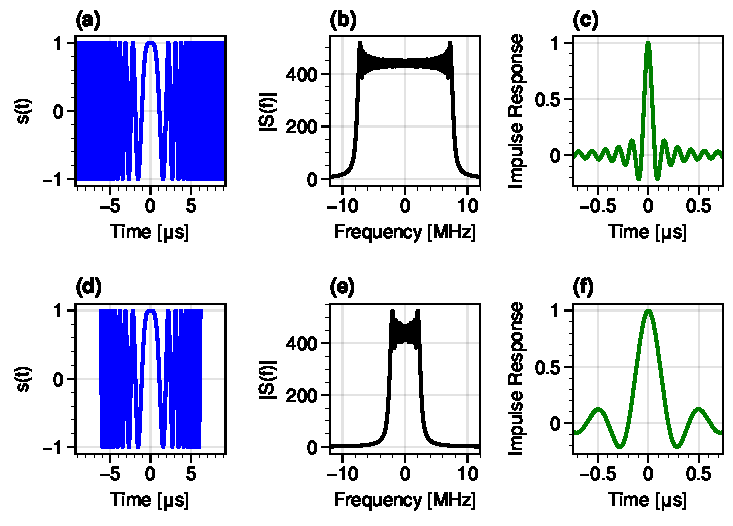
\includegraphics[width=0.99\linewidth]{figures/chapter2-sar/radar-chirp-bandwidth-ers.pdf}
%		\includegraphics[width=0.99\linewidth]{figures/chapter2-sar/radar-chirp-bandwidth-ers2.pdf}
	\caption[Range resolution from chirp compression]{
		(a) The real part of a linear frequency-modulated chirp with a duration of $\tau \approx 37.12 \mu s$ and a chirp slope $k = 4 \times 10^{11} Hz / s$.
		(b) The magnitude of the Fourier transform of the chirp is approximately a rectangle function, which shows the chirp bandwidth $BW = k \tau$ $\approx 15.5$ MHz.
		(c) Matched filtering of the returned echo from one point scatterer yields the impulse response, which shows the approximate 10 meters of range resolution (or $\sim$65 ns in time).
		(d) For a chirp with the same slope $k$ and 1/3 the duration $\tau$ the frequency bandwidth is also cut by 1/3 (e), the corresponding impulse response (f) and range resolution is 3 times worse.
	}
	\label{fig:ch2-range-compress}
\end{figure}


In the azimuth direction, the size of the radar footprint determines which ground points can be distinguished from the echo of one pulse;  this is known as the \emph{real aperture radar} (RAR) resolution. The footprint size can be written as $r \lambda / L$, which comes from the antenna's angular beam width $\lambda / L$ and the range $r$ to the target. The earliest imaging radar platforms were limited to this resolution in azimuth. For an airborne platform with a 1 meter antenna imaging at C-band, this would be a $\sim$600 meter resolution. Note that for some applications, such as military detection applications or wide-area ocean mapping \cite{Simons2007InterferometricSyntheticAperture}, this azimuth resolution is sufficient; however, the RAR resolution for spaceborne radars are on the order of 10s of kilometers, which is far too coarse for most applications.


%The advantages long wavelengths offer in terms of penetration come with compensating drawbacks. The resolution a sensor depends on the wavelength and on the size of its aperture—the mirror or lens in the case of a camera or a telescope, the antenna in a radar. If you lengthen the wavelength, you increase the size of the aperture you need in order to achieve a given resolution. To produce detailed images with radar requires a very large aperture indeed—far larger than anything a single spacecraft can offer.


\begin{figure}
	\label{fig:ch2-synth-aper}
	\centering
	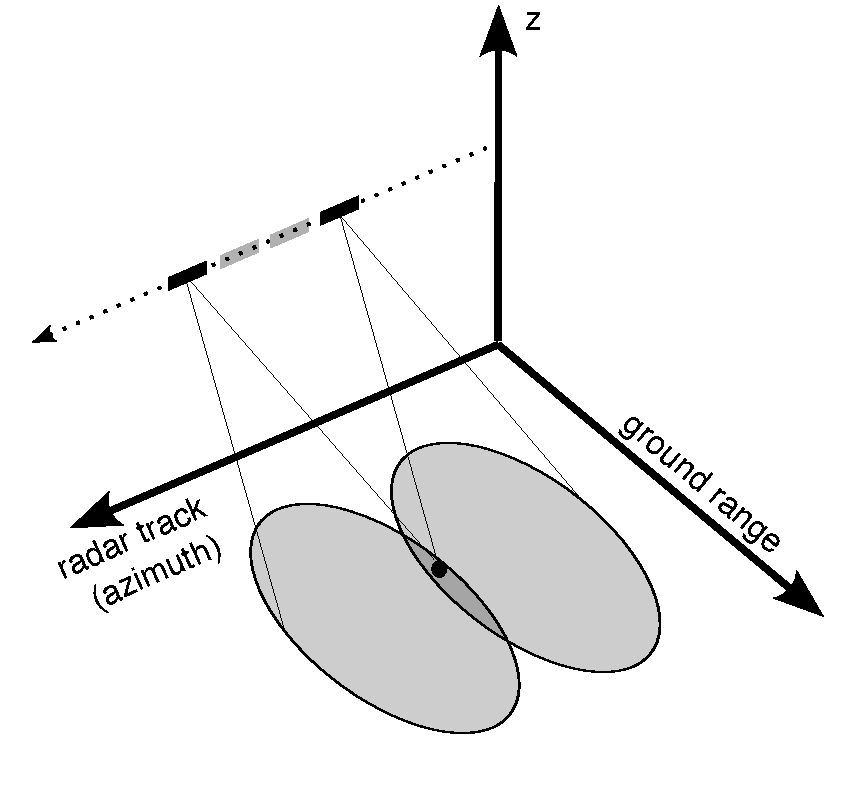
\includegraphics[width=0.8\linewidth]{figures/chapter2-sar/synth-aper2.pdf}
	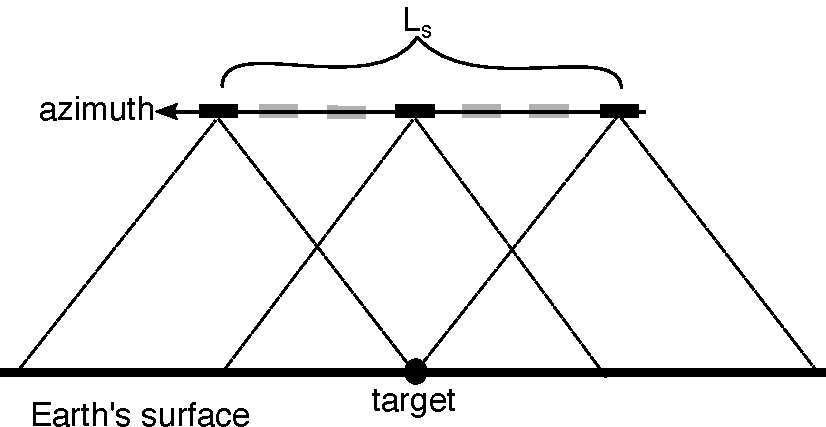
\includegraphics[width=0.99\linewidth]{figures/chapter2-sar/sar-synthetic-aperture.pdf}
	\caption[Formation of a synthetic aperture]{
		(Top) One point on the ground is illuminated by a series of pulses. Pictured here are the footprints of the first and last pulses that illuminate the point. 
		(Bottom) Side view of a series of pulses illuminating a target. By coherently processing all pulses, we can form a synthetic aperture of length $L_s$.
	}
\end{figure}


The resolution in azimuth is greatly improved by creating a \emph{synthetic aperture}, which is a technique that processes the reflected echoes coherently (i.e. using both magnitude and phase) to focus the image (Figure \ref{fig:ch2-synth-aper}).
Coherent processing is possible by carefully tracking each target's phase history, $ \phi(t) $, which is related to the range to the target $r(t)$ 
\begin{equation}
\phi(t) = -\frac{4 \pi}{\lambda} r(t)  \label{eq:ch2-phase-range}
\end{equation}
There are multiple image formation algorithms which create this synthetic aperture and use the phase history. One of the first developed and most widely today used is the range-Doppler algorithm (RDA) \citep{Wu1976DigitalSystemProduce, Cumming1979DigitalProcessingSeasat}. 
RDA uses the apparent shift in Doppler frequency due to the platform motion to create a matched filter in azimuth, similar to the matched filter used for range compression \cite{Cumming2004DigitalProcessingSynthetic}.
%RDA is a frequency-domain algorithm, since it converts the phase history 
%Which converts the range-compressed data into the frequency domain. 
An alternative to RDA is time-domain backprojection \citep{Duersch2013BackprojectionSyntheticAperture}, which provides a more exact phase compensation at the cost of being more computationally expensive.
The backprojection algorithm collects the energy from every radar pulse containing a pixel and compensates for the range-dependent phase.
%To focus an image in azimuth using backprojection,
The complex-valued radar image $S$ (also known as a \emph{single-look complex} image, or SLC) at pixel location $ (x, y) $ can be formed by summing over all pulses and applying for a range-dependent term to cancel the propagation phase:
\begin{equation}
	S(x, y) = \sum_{k} s_k \left(t_k \right) e^{j \frac{4 \pi}{\lambda} r_k(x, y)}
\end{equation}
where $j = \sqrt{-1}$, $r_k(x, y)$ is the range distance from the radar sensor to the point $ (x, y) $ at the time of the $k$th pulse, $s_k(t_k)$ is the value of the $k$th range-compressed pulse at time $t_k = r_k(x, y) / c$, and $c$ is the speed of light \citep{Zebker2018InsarMissionLevel}.
%While computationally expansive, backprojection has become more common recently due to advances in computing hardware and 
If the radar imaging geometry is known precisely so that $r_k$ can be computed for all pulses, the coherent summation can be performed for each pixel to focus the SAR image.

For all image formation methods, the final achievable azimuth resolution $\delta_{az}$ is
%Processing all echoes coherently results in a fine resolution in the azimuth direction, which is equal to the resulting that would be attainable only by a real aperture of length $2 L_s$ \citep{Cumming2004DigitalProcessingSynthetic}.
%The phase of each return echo at a time $t$ is related to the range $r$ by $\phi(t) = -\frac{4 \pi}{\lambda} r(t)$.
\begin{equation}
	\delta_{az} = \frac{L}{2}
\end{equation}
where $L$ is the physical antenna length in the azimuth direction.
%Note the this final resolution is independent of wavelength, range or platform speed.
Normal spaceborne satellites have antennas on the order of 5-10 meters, resulting in a $\delta_{az} $ between 2.5-5 meters.
The intuition behind this surprising result is that, unlike with RAR, a smaller physical antenna size $L$ leads to a wider angular beam width $ \lambda / L$. This means that a given target is illuminated for a longer time, leading to a greater number of pulses to coherently process. Thus, the azimuth resolution will actually improve with a smaller antenna size.



\section{SAR Interferometry}

Interferometric synthetic aperture radar (InSAR) refers to a broad class of applications that exploit the phase difference between two SAR images to obtain extra information beyond the 2D locations of points \citep{Bamler1998SyntheticApertureRadar}. The most common applications are generating topography maps \citep{Graham1974SyntheticInterferometerRadar, Zebker1986TopographicMappingInterferometric} and mapping surface deformation \citep{Goldstein1987InterferometricRadarMeasurement, Gabriel1989MappingSmallElevation, Li1990StudiesMultibaselineSpaceborne, Massonnet1993DisplacementFieldLanders, Rosen2000SyntheticApertureRadar}. 
The InSAR measurement is made after precisely coregistering and resampling two SLC images $S_1$ and $S_2$ to the same coordinates. The phase measurement $I_{1,2}$ is formed by multiplying the first SLC $S_1$ by the complex conjugate of the second $S_2$: 
\begin{equation}
%	I_{1,2} = S_1 S_2^{*} = A_1 A_2 e^{j \left(\phi_1 - \phi_2 \right)}  \label{eq:insar-conj-mult}
I_{1,2} = S_1 S_2^{*} = A_1 A_2 e^{j \Delta \phi_{1,2}}  \label{eq:ch2-conj-mult}
\end{equation}
where $S_k = A_k e^{j \phi_k}$, $A_k$ is the amplitude of the $k$th image, and the phase $\phi_k = -\frac{4 \pi}{\lambda} r_k$. The image $I$ is called an \emph{interferogram},  and the quantity $\Delta \phi_{1,2} \triangleq  \phi_1 - \phi_2$ is the interferometric phase.

%TODO: 
TODO: summarize SRTM, and TANDEM X missions.
%
%maybe his topography stuff....
%- summarize SRTM, and TANDEM X mission
%- after into topo, can even mention missions to emphasize importance
%- for radar interferometry... mostly mention berardino chapter.


For topography mapping, two SAR antennas are separated by a distance in the across-track direction and each acquires a SAR image simultaneously\footnote{The acquisitions can also be at different times, under the assumption that no ground deformation has occurred.} (Figure \ref{fig:ch2-insar-geometry-topo}). The baseline causes the two radars to view the same point on the ground with a slight change in angle.
The difference in phase $\Delta \phi$ between $S_1$ and $S_2$ is related to the difference in the geometrical path length from each radar to the ground.
%: $\Delta \phi = \frac{-4 \pi}{\lambda}(r_1 - r_2)$. 
This means that $\Delta \phi$ changes based on whether the satellites are viewing flat ground (Figure \ref{fig:ch2-insar-geometry-topo}a) or topography (Figure \ref{fig:ch2-insar-geometry-topo}b). Thus, with precise knowledge of the viewing geometry, the height of the topography can be inferred from the interferometric phase for each point in the interferogram \citep{Simons2007InterferometricSyntheticAperture}. 
%Note that the phase difference can be thought of as a third measurement (in addition to the location in the azimuth and range directions) that allows a reconstruction of the 3D location of each image point \cite{Simons2007InterferometricSyntheticAperture}.


\begin{figure}
	\centering
	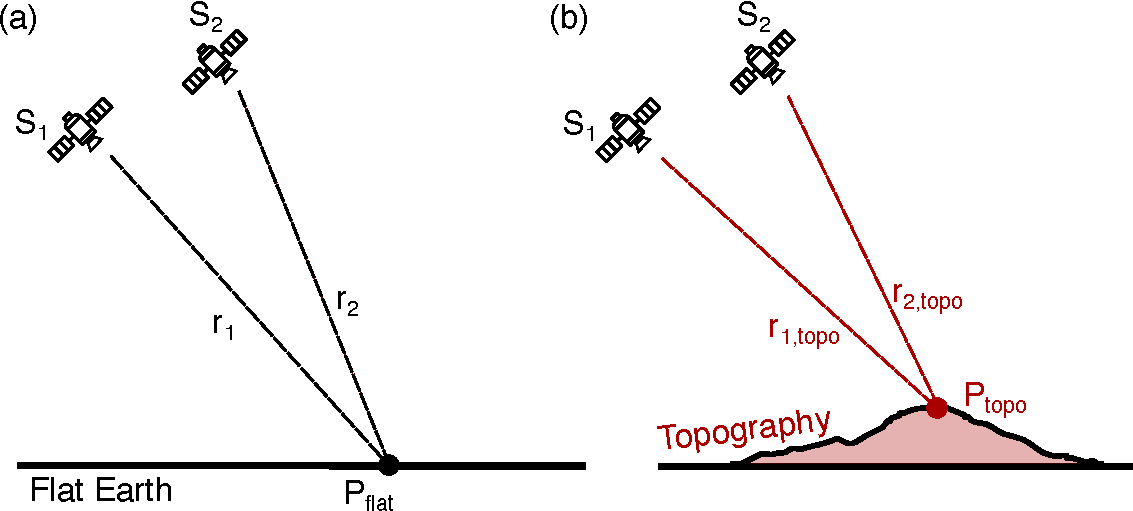
\includegraphics[width=0.99\linewidth]{figures/chapter2-sar/insar-geometry-topo.pdf}
	\caption[InSAR imaging geometry for topography mapping]{InSAR imaging geometry for topography mapping. Two SAR images, $S_1$ and $S_2$, are acquired with a slight spatial separation. The measured phase difference between $S_1$ and $S_2$ will change depending on whether we are viewing a point (a) on a flat Earth reference, or (b) at some topographic height.
%		 due to the change in look angles for each satellite.
%		(a)		 Two SAR images, $S_1$ and $S_2$, are acquired with a slight separation. The measured phase difference $\Delta \phi = \frac{4 \pi}{\lambda}(r_2 - r_1)$ results from the difference in geometric path length to the ground.
%		(b) $\Delta \phi$ changes when measuring topography due to the change in look angles for each satellite.
		 The this allows us to use the phase difference to infer the height of $P_{topo}$ above the reference Earth location $P_{flat}$.
	}
	\label{fig:ch2-insar-geometry-topo}
\end{figure}


In repeat-pass InSAR (sometimes called \emph{differential} InSAR, or DInSAR or DIfSAR)), a radar platform acquires two SAR images over an area acquired at different times, $t_1$ and $t_2$ (Figure \ref{fig:ch2-insar-geometry-defo}). Assuming that the topography is known and can be removed from the phase measurement, the remaining InSAR phase at each pixel measures the change in range along the radar LOS direction:
\begin{equation}
	\Delta \phi_{1,2} = \frac{4 \pi}{\lambda}(r_2 - r_1)   \label{eq:ch2-insar-phase-0noise}
\end{equation} 
%In the repeat pass setup, a small spatial baseline between the satellite at the two times is desired, while the topographic mapping application is more sensitive when the baseline is larger.
Since the measurement uses the phase of the propagated radar waves, it is only known modulo $2\pi$; the process of obtaining the full continuous phase is known as \emph{phase unwrapping}
\citep{Goldstein1988SatelliteRadarInterferometry, Chen2001TwoDimensionalPhase}. Note that even after phase unwrapping, the absolute number of $2\pi$ cycles from the radar to the ground is not known; thus, an unwrapped interferogram represents the surface deformation \emph{relative} to some point which is assumed to be zero.
Additionally, the description of the interferometric phase in Equation \eqref{eq:ch2-insar-phase-0noise} assumes no noise; in reality there are numerous noise sources which affect either the phase of an individual SAR acquisitions or the phase difference between pairs of images.



\begin{figure}
	\centering
	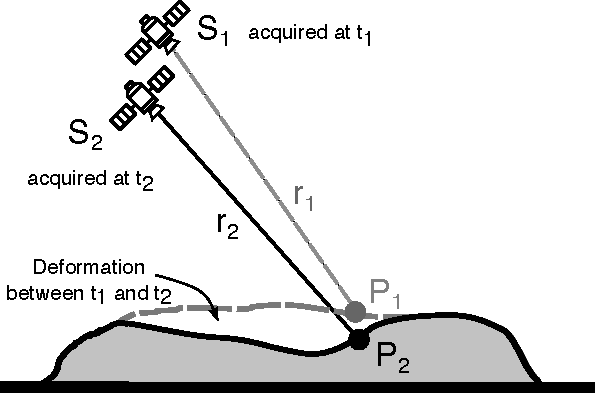
\includegraphics[width=0.9\linewidth]{figures/chapter2-sar/insar-geometry-defo.pdf}
%	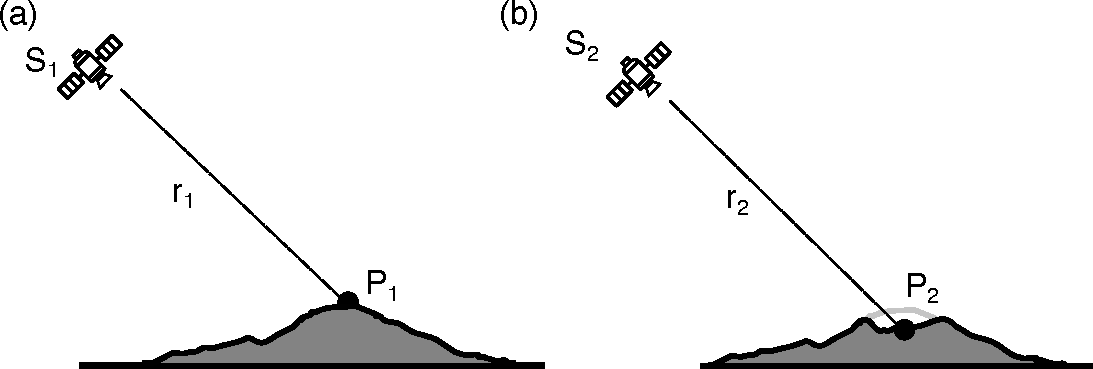
\includegraphics[width=0.99\linewidth]{figures/chapter2-sar/insar-geometry-defo-2col.pdf}
	\caption[InSAR imaging geometry for deformation mapping]{InSAR imaging geometry for deformation mapping.
		(a) Two SAR images, $S_1$ and $S_2$, are acquired at different times, before and after a ground deformation event. After removing the contribution from topography, the change in range between times $t_1$ and $t_2$ results in a measured phase change $\Delta \phi_{1,2} =  \frac{4 \pi}{\lambda}(r_2 - r_1)$.
	}
	\label{fig:ch2-insar-geometry-defo}
\end{figure}

\section{InSAR Noise Sources}
\label{sec:ch2-noise}
% decor
% atmo (further into iono/tropo, then tropo section)
%(maybe systematic for DEM/orbital,)
%thermal noise
%
After removing phase contributions from topography and satellite geometry, the phase at each pixel in an interferogram formed from SLCs $S_1$ and $S_2$ can be written as
%\citep{Zebker1992DecorrelationInterferometricRadar, Zebker1994AccuracyTopographicMaps, Zebker1997AtmosphericEffectsInterferometric, Hooper2006PersistentScatterRadar, Agram2010PersistentScattererInterferometry}
\begin{equation}
	\Delta \phi_{1, 2} = \frac{4 \pi}{\lambda} \left( \Delta d_{1,2} + \alpha_2 - \alpha_1 \right) + \Delta \phi_{iono} + \Delta \phi_{orb} + \Delta \phi_{dem} + \Delta \phi_{decor} + \Delta \phi_{unwrap} + \Delta \phi_{scat} + \Delta \phi_{n}  ,
	\label{eq:ch2-insar-noise-terms}
\end{equation}
where $ \lambda $ is the radar wavelength and $ \Delta d_{1,2} $ is the surface deformation between $S_1$ and $S_2$ along the radar LOS direction. 

The $\alpha_i$ terms represent the excess delay introduced by the neutral atmosphere on the $i$th day.
Tropospheric noise, $\Delta \phi_{tropo} \triangleq \alpha_2 - \alpha_1 $, arises from differences in pressure, temperature, or water vapor content between the two radar acquisitions \citep{Zebker1997AtmosphericEffectsInterferometric}.
%, which lead to changes in the index of refraction. 
Since tropospheric noise is the dominant noise for the West Texas study of Chapters \ref{CHAP:4-GRL}-\ref{CHAP:6-blob}, the noise is further detailed in Section \ref{sec:ch2-noise-tropo}.


Phase errors can also arise from variations in the index of refraction from due to ionospheric heterogeneities \citep{Gray2000InfluenceIonosphericElectron}. Since the ionosphere is a dispersive medium, the phase effects  $\Delta \phi_{iono}$ are dependent on radar frequency, with the effect at C-band being approximately 1/16 the effect at L-band \citep{Liang2019IonosphericCorrectionInsar}. Additionally, the dependence on frequency enables mitigation techniques which split the radar spectrum into sub-bands to calculate phase corrections \cite{Rosen2010MeasurementMitigationIonosphere}.
%with the index of refraction varying as $ \propto \frac{1}{f^2} $ \citep{Meyer2006PotentialLowFrequency}. 
%This means that 


The terms $ \Delta \phi_{orb} $ and $ \Delta \phi_{dem} $ represent systematic errors resulting from imprecise knowledge of the platform's orbital position or topographic height. Orbital errors usually appear as a planar phase ramp in stripmap acquisitions. Although these were common to see in ERS-1 or ENVISAT data, they rarely appear in Sentinel-1 data due to it's high precision orbit determination \citep{Fattahi2014InsarUncertaintyDue}. Errors in the DEM used to remove the topographic phase result in a spatial baseline-dependent phase error \citep{Fattahi2013DemErrorCorrection}. These errors often small in Sentinel-1 data due to the tight control of the repeat orbit tube, but can be significant in mountains or regions with sharp topography changes.

Decorrelation errors, $ \Delta \phi_{decor} $, arise from a loss of coherence of the phase between $S_1$ and $S_2$ due to changes in the surface dielectric properties or scattering characteristics \citep{Zebker1992DecorrelationInterferometricRadar, Michaelides2019AlgorithmEstimatingCorrecting, Ansari2018EfficientHighPrecision}. 
The correlation can be estimated from the complex coherence $\gamma $ of the interferogram \cite{Bamler1998SyntheticApertureRadar}
\begin{equation}
	\gamma = \frac{\left\langle S_1 S_2^{*} \right\rangle }{\sqrt{\left\langle S_1 S_1^{*} \right\rangle^2 \left\langle S_2 S_2^{*} \right\rangle^2}}
\end{equation}
where $ S_2^{*} $ is the complex conjugate of $ S_2 $ and $ \left\langle \cdot \right\rangle  $ denotes the statistical expectation operator. The expectation is defined as an ensemble average, but in practice it is estimated using some spatial window of pixels. 
The magnitude of this quantity $ \rho = |\gamma | $ is called the \emph{correlation} (or sometimes called the coherence), and varies from $ 0 $, indicating a complete loss of signal coherence, to $ 1 $, indicating perfectly correlated radar echoes.
%Decorrealtion 
When the correlation is very low, the phase unwrapping processing may fail and produce patches of pixels which have $2 \pi$ offsets from the correct value. These are known as phase unwrapping errors, $ \Delta \phi_{unwrap}  $. For study areas which regularly have strong decorrelation (e.g. agricultural areas), the technique known as persistent scatterer interferometry is used to overcome decorrelation by locating the phase-stable pixels which maintain coherence over long periods of time \citep{Ferretti2001PermanentScatterersSar, Agram2010PersistentScattererInterferometry, Hooper2006PersistentScatterRadar}.
%Note that because the angle of $\gamma$ is the interferometric phase, $\gamma$ may be considered the primary interferometric observable \citep{Michaelides2020QuantifyingPermafrostProcesses}.




The term $ \Delta \phi_{scat} $ represents phase introduced by changes to the surface and subsurface scattering properties. This term is separated from the random decorrelation noise since it has recently been shown that systematic, non-random effects can occur from changes to subsurface dielectric properties (e.g. from changes to soil moisture) \citep{Zan2014SarInterferometricModel, Zan2015PhaseInconsistenciesMultiple, Zwieback2016InfluenceSoilMoisture, Michaelides2020QuantifyingPermafrostProcesses}.
Although this term is noise for the application of deformation monitoring
\citep{Michaelides2019AlgorithmEstimatingCorrecting, Ansari2021StudySystematicBias}, other recent efforts have attempted to use this term to invert for changes to soil moisture \citep{Zwieback2017SoilMoistureEstimation, Zan2018VegetationSoilMoisture}. 
Finally, $ \Delta \phi_n $ represents other residual noise terms, including thermal noise from the radar antenna system, that are typically an order of magnitude smaller than the other errors listed.


Although these effects have been presented as noise sources for the application of deformation monitoring, they can be the signal of interest in other InSAR applications. For example, the presence of decorrelation indicates a change to the scattering surface properties and can be used for coherent change detection \citep{Simons2007InterferometricSyntheticAperture, Jung2016CoherentChangeDetection}, and the phase variations from the troposphere have been used for atmospheric mapping and meteorological purposes \citep{Hanssen1999HighResolutionWater, Liu2012SatelliteRadarInterferometry}.

% include orbital errors, phase decorrelation, unwrapping errors, DEM inaccuracies, ionospheric and tropospheric artifacts,
% and other residual noise terms that are typically an order of magnitude smaller than the error terms listed here.
%\begin{table}
%\begin{longtable}[]{@{}llcc@{}}
%	\toprule
%	Noise Symbol & Name & InSAR or SAR & asdf\tabularnewline
%	\midrule
%	\endhead
%	\phi_{orb} & & &\tabularnewline
%	\bottomrule
%\end{longtable}
%\end{table}


\subsection{Visual Example of Common Noise Sources}
\label{sec:ch2-noise-example}

In high signal to noise ratio (SNR) interferograms (e.g. for large magnitude earthquakes such as \cite{Massonnet1993DisplacementFieldLanders}), one can estimate the deformation magnitude by simply ``counting the fringes'' (i.e. visually estimating the number of $ 2 \pi $ cycles) and multiplying by $\lambda/2$. However, it is more common for an interferogram to contain many visual features corresponding to noise terms in Equation \eqref{eq:ch2-insar-noise-terms}. These noise sources can often be visually identified by InSAR experts, but they can add considerable difficulty for newer users without background knowledge of the study area.

\begin{figure}[!htbp]
	\centering
%	\includegraphics[width=1.0\textwidth]{figures/chapter2-sar/hawaii-example.pdf}
	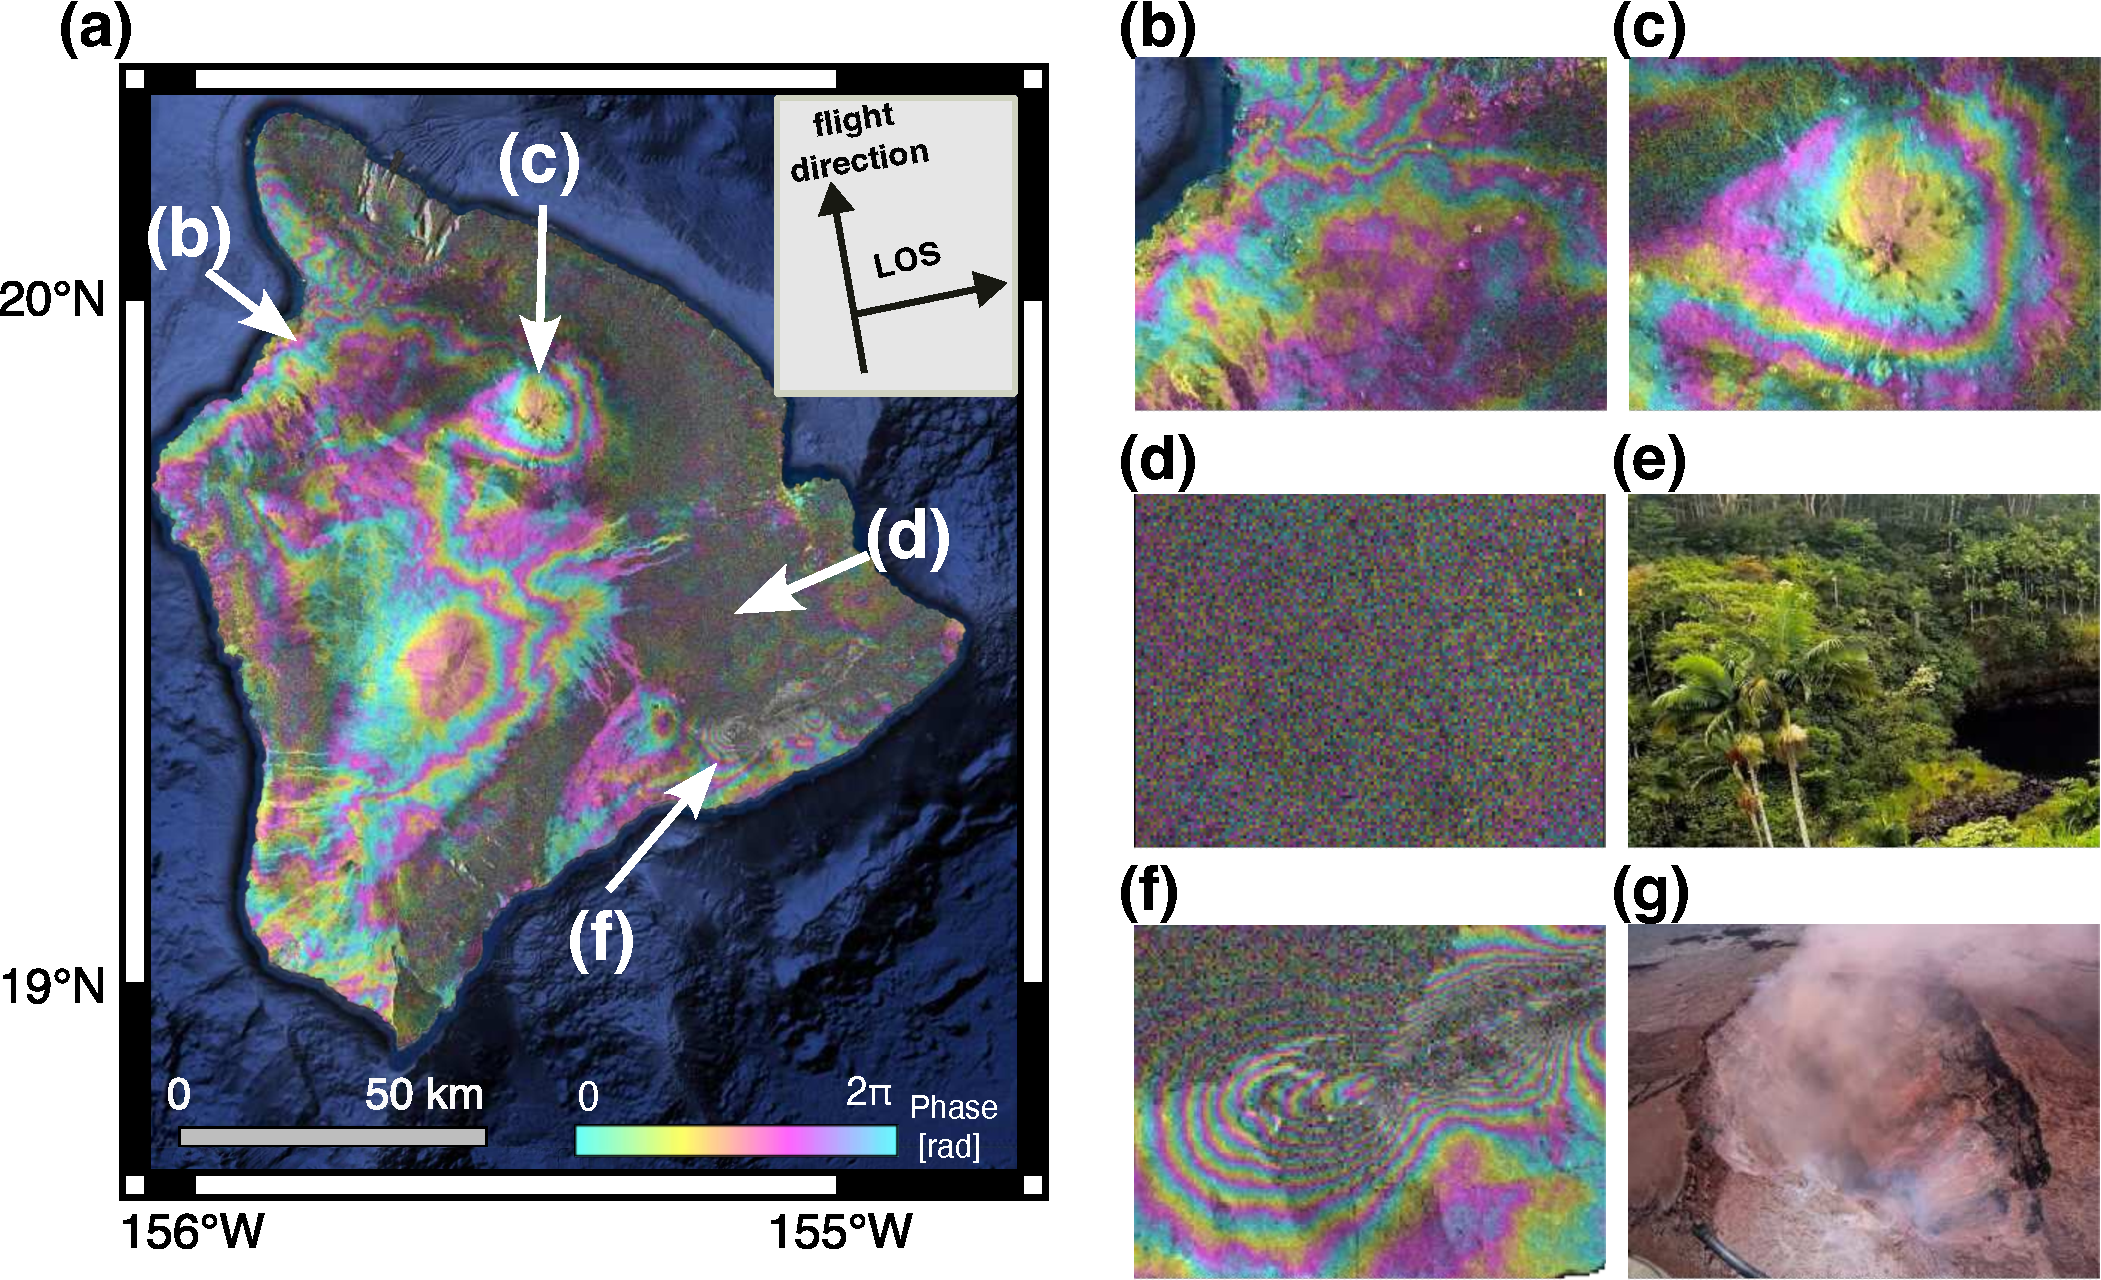
\includegraphics[width=1.0\textwidth]{figures/chapter2-sar/hawaii-example-small.pdf}
	\caption[Sentinel-1 interferogram over Hawaii showing common noise sources, along with 2018 eruption deformation]{
		(a) Sentinel-1 interferogram (ascending path 124) from April 20th, 2018 to May 2nd, 2018 over Hawaii, spanning the beginning of the 2018 K'\=ilauea eruption.
		Each colored phase cycle of $2\pi$ radians indicates a range change of 2.7 cm along the radar line-of-sight, which can be caused by real surface deformation or a noise source.
		(b) The dense fringes near the coast are caused by turbulent tropospheric noise (see Section \ref{sec:ch2-noise-tropo-mitigate}).
		(c) Stratified tropospheric noise on the peak of Mauna Kea, the tallest peak on Hawaii at 4,207 m, causes a concentric ring pattern. This pattern is also visible on Mauna Loa in the center of the island, where the phase is strongly correlated with topographic height. See Section \ref{sec:ch2-noise-tropo-mitigate} for further details.
		(d) An example of decorrelation noise caused by dense tropical rain forests (e) located on windward side of the island.
		(f) Real deformation of $ \sim 30-40 $cm around the Pu'u '\=O'\=o volcanic cone to the east of K'\=ilauea. In this case, the ground was subsiding down and to the southeast as magma flowed away from Pu'u '\=O'\=o.
		%		The signal of interest in this interferograms, the collapse of the Pu'u '\=O'\=o caldera
		(g) An aerial photo of Pu'u '\=O'\=o shows the caldera collapse on April, 30th, 2018 after magma migrated eastward underground (image source: HVO / USGS).
	}
	\label{fig:ch2-hawaii-example}
\end{figure}

To illustrate several common noise sources, Figure \ref{fig:ch2-hawaii-example} shows a Sentinel-1 interferogram of the Big Island of Hawaii from April 20th, 2018 to May 2nd, 2018. 
This time period spans the beginning of the 2018 Kilauea eruption during which a large subsidence event occurred from subsurface magma flow. However, the diversity in weather conditions and topography lead to many noise sources in most interferograms of Hawaii.
For example, the coastal region in Figure \ref{fig:ch2-hawaii-example}b contains dense fringes which could be mistaken as deformation, but in fact is due to turbulent tropospheric noise (further explained in Section \ref{sec:ch2-noise-tropo-mitigate}).
The large elevation changes on Mauna Loa and Mauna Kea in the center of the island lead to stratified tropospheric noise (see Section \ref{sec:ch2-noise-tropo-mitigate}) which creates a concentric ring pattern that is the same shape as a subsidence bowl (Figure \ref{fig:ch2-hawaii-example}c).
An example of decorrelation noise occurs on the windward side of the island (Figure \ref{fig:ch2-hawaii-example}d), which contains many dense tropical rain forests (Figure \ref{fig:ch2-hawaii-example}e). 

Finally, a real deformation feature of $ \sim 30-40 $ cm occurred near the Pu'u '\=O'\=o volcanic cone (Figure \ref{fig:ch2-hawaii-example}f).
In this case, the ground subsided down and to the southeast as magma flowed away from Pu'u '\=O'\=o (Figure \ref{fig:ch2-hawaii-example}g).
One can estimate the magnitude of deformation by counting the number of cycles in the interferogram in the zoomed-in region of Figure \ref{fig:ch2-hawaii-example}f and multiplying by 2.7 cm.
However, even this analysis can be difficult due to the high spatial frequency of the fringes.
In this case, the deformation magnitude can be verified using nearby permanent GPS stations.

%These areas show heavy decorrelation at the Sentinel-1 C-band wavelength of 5.5 cm (Figure \ref{fig:ch2-hawaii-example}d). 

%
%Two days after the interferogram on May 4, a  M$_w$ 6.9 earthquake struck the south flank of the Lower East Rift Zone, just south of the zoom.


% at the Sentinel-1  
%brief fissure eruption occurred on the west flank of the Puʻu ʻŌʻō cone on April 30, 20181. Over the next few days, earthquakes migrated eastward into the LERZ and rift-normal displacements were recorded by GPS instruments, signaling large-scale injection of magma downrift of Puʻu ʻŌʻō. Magma reached the surface in Leilani Estates subdivision on May 3, marking the onset of the LERZ eruption (Fig. 1a)

%1. Table: noise, specific to ifg or SAR, max variance?, common?



\section{Tropospheric Noise}
\label{sec:ch2-noise-tropo}


% SEASONAL plots...??

The conversion between phase two-way distance from ground to satellite in Equation \eqref{eq:ch2-phase-range} assumes that the electromagnetic waves travel though a homogeneous medium with constant velocity. In reality, they travel through a spatially inhomogenous atmosphere with variable index of refraction $n$, where $n$ relates to the phase velocity $v$ and speed of light in a vacuum $c$ by $n = c/v$ \citep{Zebker1997AtmosphericEffectsInterferometric, Hanssen2001RadarInterferometryData, Liu2012SatelliteRadarInterferometry}.  Since $n$ is always real and slightly greater than $1$ for Earth's neutral atmosphere, it is more common to describe fluctuations using the \emph{refractivity} $N = 10^{6}(n - 1)$, which is the additional refractive index beyond unity.
Writing $N$ as $N(x,y,z)$ to emphasize the 3D variation, we can express the excess delay $D$ caused by the propagation through the atmosphere as
\begin{equation}
	D = 10^{-6} \int_{s} N(x, y, z) ds
\end{equation}
where $ds$ is the incremental slant length, and the integration runs along the radar line of sight. The excess delay adds an additional phase of $\phi = - \frac{4 \pi}{\lambda} D$ to a radar image acquired with the given atmospheric conditions.
%, and each interferogram contains a phase difference of two SLCs (i.e. the phase contains the difference from two atmospheric conditions).

The refractivity of the troposphere is commonly decomposed into a hydrostatic, wet, and liquid component \citep{Hanssen2001RadarInterferometryData, Bekaert2015StatisticalComparisonInsar}:
\begin{equation}
	N = \left(k_1 \frac{P}{T} \right)_{\text{hyd}} + \left( k_2^{'} \frac{e}{T} + k_3  \frac{e}{T^2}   \right)_{\text{wet}} + \left(k_4 W \right)_{\text{liquid}}
\end{equation}
where $ P $ is the total atmospheric pressure in hPa, $ T $ is the atmospheric temperature in Kelvin,  $ e $ is the partial pressure of water vapor in hPa, and W is the liquid water content of clouds in g/m$^3 $ 
The coefficients $ k_1, k_2^{'}, k_3 $ and $ k_4 $ are constants estimated from laboratory measurements, commonly taken to be $ k_1 = 77.6$ , $ k_2^{'} = 23.3 $, $ k_3= 3.75 \cdot 10^5 $, and $ k_4 = 1.45 $ from \cite{Smith1953ConstantsEquationAtmospheric} and \cite{Solheim1999PropagationDelaysInduced}.
%Although absolute delays decrease at lower altitudes as the signal travels through more of the atmosphere, an interferogram always measures a \emph{difference} of delays from two SAR acquisitions, and hence difference of refractivity. This means that although the hydrostatic delay is of the order of a few meters and the wet delay is $ \sim10$s of centimeters, phase artifacts in interferograms are more commonly caused by the spatial variations of the wet component of refractivity \citep{Zebker1997AtmosphericEffectsInterferometric, Hanssen2001RadarInterferometryData}. 
The hydrostatic delay is on the order of a few meters; however, it varies slowly laterally and it is often assumed to be vertically stratified (i.e. varying only with elevation) for areas smaller than $100 \times 100$ km \citep{Doin2009CorrectionsStratifiedTropospheric}.
The wet component, caused by variations in water vapor content, is smaller in absolute terms ($ \sim10$s of centimeters) but has significant lateral variations at short length scales. The delay from the liquid component is often negligible (1-2 millimeters or less) but can be several centimeters in the presence of tall cumulonimbus clouds \citep{Liu2012SatelliteRadarInterferometry}.
For the purposes of InSAR analysis, noise from tropospheric delay is usually divided into a stratified component, which correlates with height \citep{Hanssen2001RadarInterferometryData, Doin2009CorrectionsStratifiedTropospheric}, and a turbulent component that is random at time scales longer than a day \citep{Emardson2003NeutralAtmosphericDelay, Onn2006ModelingWaterVapor}. 

%The hydrostatic delay is of the order of a few meters (Bevis et al., 1996) and the wet delay is usually not larger than 0.3 m (Elgered, 1982).
%The delay caused by droplets depends on the cloud type..
%ccording to Eq. (2.2.10) and the values of W listed in Tab. 2.1, significant delay up to 3 cm can be caused by the liquid water in vertical clouds, i.e., cumulonimbus (thunder clouds), which usually have a relatively limited horizontal size (< 10 km) and a large vertical extent and liquid water content. These clouds are typically generated by thermal convection or frontal lifting (Stull, 1995; Hanssen, 2001) \cite{Liu2012SatelliteRadarInterferometry}.


\subsection{Correction and Mitigation Strategies for Tropospheric Noise}
\label{sec:ch2-noise-tropo-mitigate}

%\subsection{Stratified Tropospheric Noise}
%\label{sec:ch2-noise-tropo-strat}
%\subsection{Turbulent Tropospheric Noise}
%\label{sec:ch2-noise-tropo-turb}

%Figure- GOES for storm cloud, and for weather front. Maybe there is where cite the reason why can't correct always.



Previous studies have made advances in correcting for the stratified component of tropospheric noise.  Several empirical approaches have been developed to fit linear or power-law relationships between the unwrapped phase and elevation of coherent pixels within unnwrapped interferograms \citep{Elliott2008InsarSlipRate, Lauknes2011InsarTroposphericStratification, Bekaert2015SpatiallyVariablePower, Zebker2021AccuracyModelFree, Murray2021ClusterBasedEmpirical}. Under the assumption that the deformation does not correlate with topography, these approaches can be effective and simple to implement. For example, Figure \ref{fig:ch2-hawaii-strat} shows the unwrapped interferograms from the area on top of Mauna Kea indicated in Figure \ref{fig:ch2-hawaii-example}c. Although the interferogram appears to show a bowl shape deformation (Figure \ref{fig:ch2-hawaii-strat}a), the phase is actually closely correlated with the topography (Figure \ref{fig:ch2-hawaii-strat}b-c). Fitting and removing a linear trend from the phase vs. elevation plot mitigates the stratified atmospheric noise in this case. However, these approaches can be less effective in regions with multiple weather patterns where the phase-elevation correlation can vary dramatically in space \cite{Murray2021ClusterBasedEmpirical}.

\begin{figure}[!h]
	\centering
	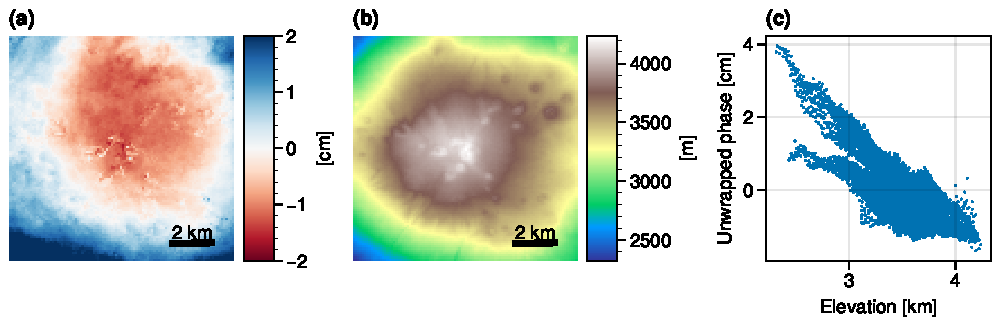
\includegraphics[width=1.0\textwidth]{figures/chapter2-sar/hawaii-strat-zoom.pdf}
	\caption[Stratified tropospheric noise over Hawaii]{
		(a) Unwrapped version of interferogram from Figure \ref{fig:ch2-hawaii-example}c, zoomed in to the top of Mauna Kea.
		(b) SRTM DEM heights for same area as (a)
		(c) Scatterplot of unwrapped phase (converted to centimeters) from panel (a) vs heights from panel (b) for all pixels.
	}
	\label{fig:ch2-hawaii-strat}
\end{figure}


Many efforts have advanced stratified noise correction using auxiliary sources of data, including global atmospheric models (GAMs) \citep{Doin2009CorrectionsStratifiedTropospheric, Jolivet2011SystematicInsarTropospheric, Jolivet2014ImprovingInsarGeodesy, Cao2021AdvancedInsarTropospheric}, GPS zenith delay measurements \citep{Onn2006ModelingWaterVapor, Yu2017GenerationRealTime}, and external satellite measurements from sensors such as the Moderate Resolution Imaging Spectroradiometer (MODIS) \citep{Li2005InterferometricSyntheticAperture, Barnhart2013CharacterizingEstimatingNoise} or the Medium Resolution Imaging Spectrometer (MERIS)  \citep{Ding2008AtmosphericEffectsInsar}.
Several authors have attempted to create off-the-shelf correction services or toolboxes from these data sources. For example,	
\cite{Yu2018GenericAtmosphericCorrection} combined information from GAMs and available GPS zenith delay measurements to create the Generic Atmospheric Correction Online Service (GACOS) for estimating tropospheric noise in InSAR data. \cite{Maurer2021RaiderRaytracingAtmospheric} created a library for ray-tracing the LOS paths through GAM-predicted delays to create correction products.

%Due to the limited spatial and temporal resolution of weather models and GPS data, GACOS is more effective in removing the stratified tropospheric noise \citep{Doin2009CorrectionsStratifiedTropospheric} than the random turbulent tropospheric noise \citep{Emardson2003NeutralAtmosphericDelay}. 
%We found that GACOS does not produce substantial corrections in most Sentinel-1 West Texas interferograms for areas outside the main area of interest (e.g. Figure \ref{fig:GACOS} (a)-(c)).


Below we illustrate correction attempts for two Sentinel-1 (path 78) interferograms over West Texas using GAM predictions (Figures \ref{fig:ch2-tropo-correct-wave}, \ref{fig:ch2-tropo-correct-storm}). 
The corrections are produced by the Raytracing Atmospheric Delay Estimation for Radar (RAiDER) library \citep{Maurer2021RaiderRaytracingAtmospheric}, which generates a troposphere correction product from a user-selected GAM. Here we use NASA's Global Modeling and Assimilation Office (GMAO) reanalysis weather models, which are interpolated by the RAiDER library to the same pixel spacing as the interferograms ($\sim$ 500 m here). We also compare the weather conditions that are visible at the secondary SAR acquisition time \footnote{For both Figures \ref{fig:ch2-tropo-correct-wave}, \ref{fig:ch2-tropo-correct-storm}, the earlier SAR acquisition time occurs during winter, which is after sunset for Sentinel-1 path 78 over West Texas. Most of the tropospheric noise in these winter-to-summer interferograms comes from the summer SAR acquisition.} using the Geostationary Operational Environmental Satellites (GOES).

In the first example, the secondary acquisition of the interferogram contains a summer thunderstorm (Figure \ref{fig:ch2-tropo-correct-storm}a). The tall cumulonimbus clouds create areas of excess delay of $>10$ cm to the interferogram over short scale lengths (under 5 km, Figure \ref{fig:ch2-tropo-correct-storm}b). 
Note that the different imaging geometries of the Sentinel-1 satellites in low Earth orbit and the GOES satellites in geostationary orbit mean the pixels of Figure \ref{fig:ch2-tropo-correct-storm}a and Figure \ref{fig:ch2-tropo-correct-storm}b do not fully align, but cover approximately the same area.
The $\sim 5$ km storm cells are too small for the GMAO weather model to predict, due to its $\sim30$ km grid spacing (Figure \ref{fig:ch2-tropo-correct-storm}c). Thus, the corrected inteferogram still contains most of the turbulent noise from the storm (Figure \ref{fig:ch2-tropo-correct-storm}d).

\begin{figure}[!ht]
	\centering
	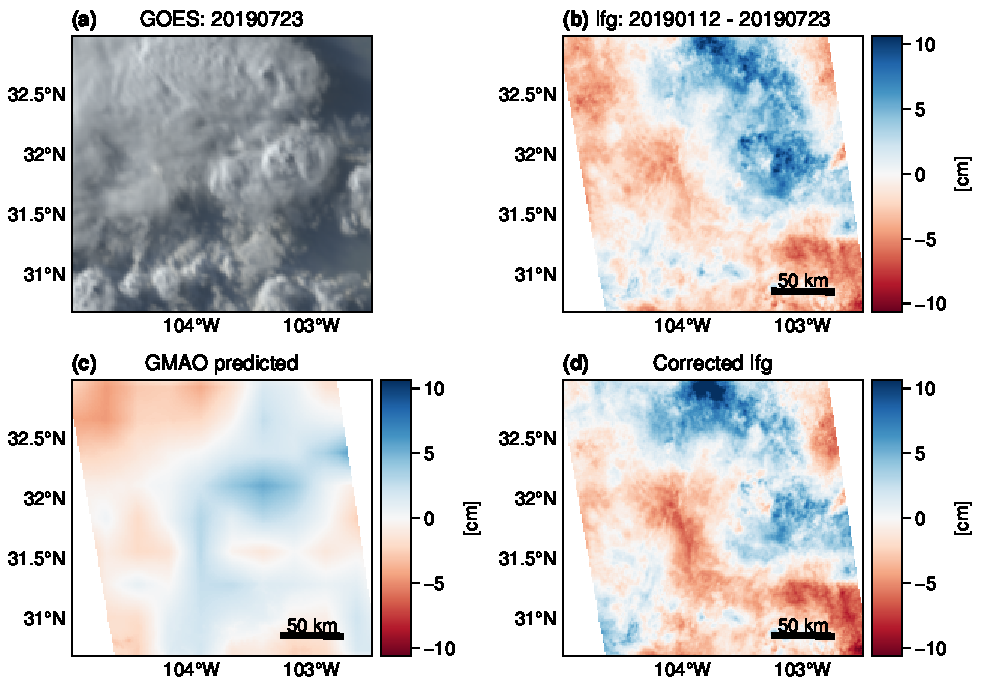
\includegraphics[width=1.0\textwidth]{figures/chapter2-sar/figure_tropo_correct_storm.pdf}
	\caption[West Texas tropospheric correction for thunderstorm]{
		(a) Weather conditions visible from the GOES satellite on July 23rd, 2019 at the same time as the Sentinel-1 acquisition
		(b) Unwrapped interferogram from Jan. 12, 2019 to July 23, 2019. Blue indicates an increase in relative LOS delay
		(c) Tropospheric correction predicted from delays computed by the GMAO weather model.
		(d) Corrected interferogram (panel (b) - panel (c))
	}
	\label{fig:ch2-tropo-correct-storm}
\end{figure}

The second example illustrates strong tropospheric noise resulting from a low-pressure front moving from northwest to southeast, which creates a $\sim 20$ cm decrease in LOS delay compraed to the southeast portion of the interferogram (Figure \ref{fig:ch2-tropo-correct-wave}b). Note that this pressure front is not visible in the visible spectrum of the GOES image (Figure \ref{fig:ch2-tropo-correct-wave}a), but is present in the GMAO weather model (Figure \ref{fig:ch2-tropo-correct-wave}c). Although the RMS noise of the corrected interferogram drops from 6.1 cm to 2.6 cm, the slight temporal differences of the model output and interferogram acquisition times lead to only a partial correction of the tropospheric pattern.

\begin{figure}[!h]
	\centering
	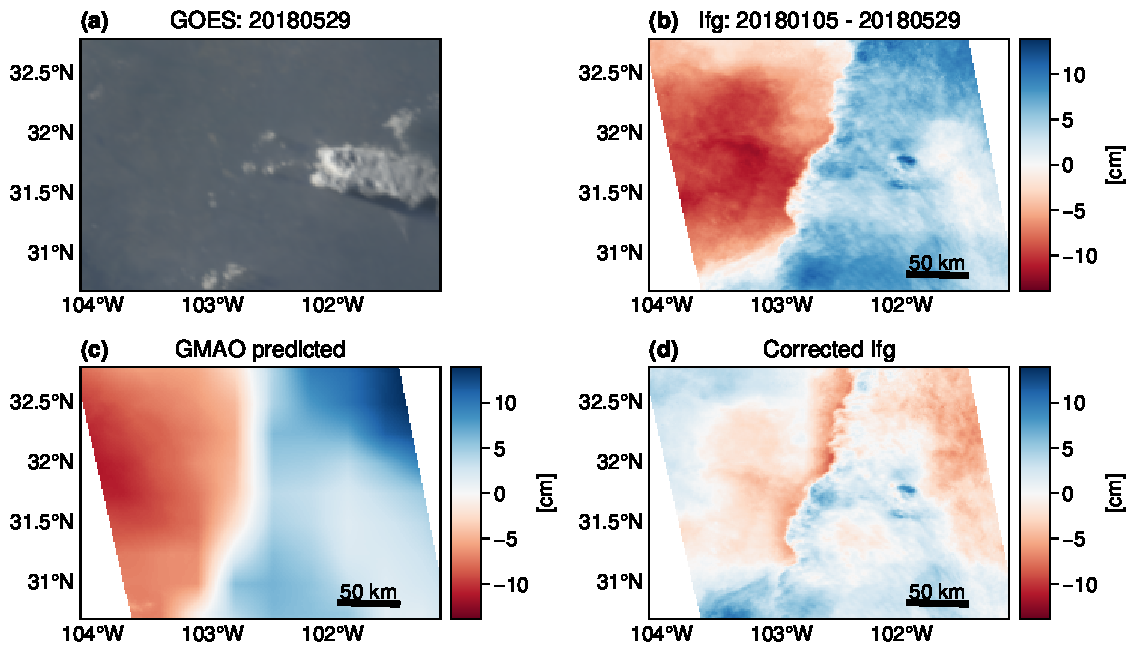
\includegraphics[width=1.0\textwidth]{figures/chapter2-sar/figure_tropo_correct_wave.pdf}
	\caption[West Texas tropospheric correction attempt for pressure front]{
		(a) Weather conditions visible from the GOES satellite on May 29th, 2018 at the same time as the Sentinel-1 acquisition.
		(b) Unwrapped interferogram from Jan. 5, 2018 to May 29, 2018. Blue indicates an increase in relative LOS delay.
		(c) Tropospheric correction predicted from delays computed by the GMAO weather model.
		(d) Corrected interferogram (panel (b) - panel (c))
	}
	\label{fig:ch2-tropo-correct-wave}
\end{figure}

While these correction methods show promise in certain study areas, the spatial and temporal resolution is often too low to correct for noise from severe weather or turbulent mixing of water vapor. Therefore, most methods for mitigating the turblent tropospheric noise rely on time series methods that exploit the uncorrelated temporal characteristics of the noise.
% on the atmospheric delay being uncorrelated for time scales longer than $\sim 6$ hours \cite{Emardson2003NeutralAtmosphericDelay}.


%
%\begin{figure}
%	\centering
%	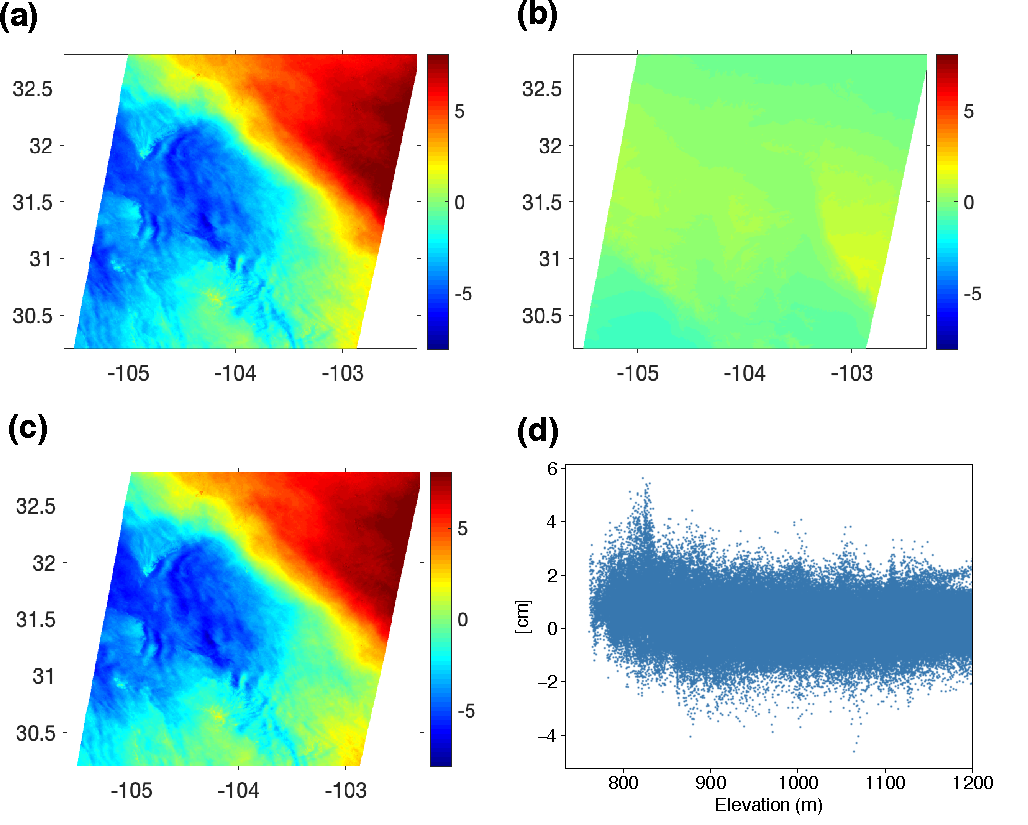
\includegraphics[width=\textwidth]{paper1-permian/figures/supplement/figureS4-gacos.pdf}		
%	\caption[GACOS tropospheric corrections]{(a) LOS measurements (in cm) of a descending interferogram (20150127-20150220) before the GACOS correction. (b) GACOS tropospheric correction (in cm) for the 20150127-20150220 interferogram \citep{Yu2018InterferometricSyntheticAperture}. (c) LOS measurements (in cm) of a descending interferogram (20150127 - 20150220) after the GACOS correction. (d) LOS measurements (in cm) of the 20150127-20150220 interferogram vs. the Digital Elevation Model (DEM).}
%	\label{fig:GACOS}
%\end{figure}


%In Chapters \ref{CHAP:4-GRL} and \ref{CHAP:5-robust-ts}, we 


\section{InSAR Time Series}
\label{sec:ch2-insar-ts}

%There are many techniques which fall under the umbrella of InSAR time series techniques, (sometimes called ``multi-temporal InSAR'' or MT-InSAR).
Since many noise sources cannot be distinguished from deformation in a single interferogram (e.g. Figure \ref{fig:ch2-hawaii-example}), it is common to analyze multiple interferograms to quantify and mitigate InSAR noise sources.
InSAR time series techniques (sometimes called ``multi-temporal InSAR'' or MT-InSAR) are a class of methods for extracting information about the temporal evolution of surface deformation or other geophysical parameters of interest.  Most multi-temporal methods have generally been classified as belonging to one of the following categories: 1) stacking (averaging) \citep{Zebker1997AtmosphericEffectsInterferometric, Sandwell1998PhaseGradientApproach}, 2) small-baseline approaches \citep{Berardino2002NewAlgorithmSurface}, or 3) persistent-scatterer (PS) methods \citep{Ferretti2001PermanentScatterersSar, Hooper2006PersistentScatterRadar}. In the past decade, a fourth category of ``phase-linking'' approaches have been popularized by the SqueeSAR algorithm \citep{Ferretti2011NewAlgorithmProcessing}; these are based on optimizations or decompositions of the complex covariance matrix of SAR image stacks \citep{Guarnieri2008ExploitationTargetStatistics, Fornaro2015CaesarApproachBased, Ansari2018EfficientHighPrecision}. Methods (3) and (4) have shown success in extracting high-precision estimates of interferometric phase where decorrelation is the dominant noise source (e.g. in local, high-rate deformation, \citep{Tebaldini2010MethodsPerformancesMulti}); in the following section, we focus on (1) and (2).


For deformation signals which occur as a transient event 
%(which includes all processes quicker than one SAR acquisition interval) 
or with a constant rate, stacking consists of averaging multiple interferograms (possibly with different weights for each interferogram) which all contain the deformation signal \citep{Simons2007InterferometricSyntheticAperture, Zheng2019ImagingCascadiaSlow}. 
%Stacking approaches are the simplest conceptually and the earliest developed to mitigate tropospheric noise. 
For example, suppose an earthquake occurred at a known date, and we would like to estimate the coseismic displacement $\theta$ that occurred using a set of $M$ interferograms which all span the earthquake date. For each ground pixel, we can collect the phase difference measurements into a vector $\bm{\Delta \phi} \in \mathbb{R}^{M} $.
%\begin{equation}
%	\bm{\Delta \phi} = \left[ \Delta \phi_{1,2}, \Delta \phi_{1,3} , \ldots  \right]^T
%\end{equation}
To estimate the $\theta$, the simplest stacking solution is
\begin{equation}
	\theta = \frac{\lambda }{4 \pi} \frac{1}{M} \sum_i^M \bm{\Delta \phi}_i ,
	\label{eq:ch2-stacking-1}
\end{equation}
%consists of the $M$ phase differences for one ground pixel location, 
where $\bm{\Delta \phi}_i$ is $i$th element of the measurement vector, and the factor $  \frac{\lambda }{4 \pi} $ converts the phase from radians to centimeters.
For constant rate ground deformation, one approach based on \citep{Sandwell1998PhaseGradientApproach} to calculate the average LOS velocity $v_{avg}$ of each ground pixel is to compute
\begin{equation}
%	v_{avg} = \frac{\lambda }{4 \pi} \frac{\sum_{i \in G} d_i}{\sum_{i \in G} t_i}
	v_{avg} = \frac{\lambda }{4 \pi} \frac{\sum_i \bm{\Delta \phi}_i}{\sum_i \bm{\Delta t}_i }
	\label{eq:ch2-stacking-2}
\end{equation}
where $ \bm{\Delta t}_i $ is the temporal baseline of the $i$th interferogram (i.e. the time span $t_k - t_j$  for interferogram $ \Delta \phi_{j, k} $). %between SAR acquisitions at $t_j$ and $t_k$
%As noted by \cite{Simons2007InterferometricSyntheticAperture}, this method is equivalent to converting the interferogram measurements to rates and performing an averaging weighted by the respective time span.



% Yunjun thesis: the vector of interferometric phase residual that does not fulfill the zero phase closure of interferogram triplets. It includes the decorrelation noise, phase contribution due to the change of dielectric properties of ground scatterers such as soil moisture (De Zan et al., 2014; Morrison et al., 2011), processing inconsistency such as filtering, multilooking, coregistration and interpolation errors (Agram and Simons, 2015; Hanssen, 2001), and/or phase-unwrapping errors.

%An alternative objective function to solve equation (2.1) is minimizing the L2-norm of the residual of phase velocity of adjacent acquisitions (equation (16) in Berardino et al. (2002)). Optimizations with both objective functions give nearly identical solutions for a fully connected network



The Small Baseline Subset (SBAS) approach from \cite{Berardino2002NewAlgorithmSurface} formulates a linear estimation problem to solve for the phase at each SAR acquisition.
Suppose that the $M$ interferograms are formed from $N$ SAR acquisitions, where $ \frac{N}{2} \leq M \leq \frac{N(N - 1)}{2} $, and all interferograms have been unnwrapped and zero-referenced to a common location.
To solve for the LOS phase delay for each SAR acquisition $ \bm{\phi} = \left[\phi_0, \phi_1, \ldots, \phi_{N-1} \right]^T $, 
%we organize the system of equations as
we write the functional model of the linear system as
\begin{equation}
	\bm{A \phi} = \bm{\Delta \phi} + \bm{\epsilon} . \label{eq:ch2-sbas-A}
\end{equation}
where  $\bm{A}$ is the system design matrix, and $ \bm{\epsilon}  $ is the vector of interferogram-specific noise sources (e.g. $ \Delta \phi_{decor}, \Delta \phi_{unwrap}, \Delta \phi_{scat}, \Delta \phi_{n} $ from Equation \eqref{eq:ch2-insar-noise-terms}).
The matrix $\bm{A}$ is an incidence-like matrix where the row corresponding to measurement $ \Delta \phi_{j,k} \triangleq \phi_k - \phi_j $ has $1$ in the $k$th column and $-1$ in the $j$th column.
% (for all $j>0$).
Since interferograms are relative measurements, the first date's phase cannot be constrained and is conventionally taken to be $\phi_0 = 0$. Therefore, we omit the first column of the $ \bm{A} $ matrix containing $-1$ entries corresponding to $\phi_0$, leaving $N-1$ remaining terms in the unknown vector $ \bm{\phi} = \left[\phi_1, \ldots, \phi_{N-1} \right]^T $.
When $ \bm{A} $ is full column rank, the solution for $ \bm{\phi} $ can be obtained through least squares, $ \bm{\phi} = (\bm{A}^T \bm{A})^{-1}\bm{A}^T \bm{\Delta \phi}
 $, equivalent to minimizing the $L_2$ norm of the residual vector $\norm{\bm{A \phi} - \bm{\Delta \phi}}^2_2 $.

A common alternative to Equation \eqref{eq:ch2-sbas-A} is to solve for the phase velocity between each SAR acquisition $\bm{v} = [v_1, \ldots, v_{N-1}]^T$ where $ v_i = (\phi_i - \phi_{i-1})/(t_i - t_{i-1} ) $.
The linear system is now written as
\begin{equation}
	\bm{B v} = \bm{\Delta \phi} + \bm{\epsilon}, \label{eq:ch2-sbas-B}
\end{equation}
where the row of $\bm{B}$
corresponding to measurement $ \Delta \phi_{j,k} $ has $t_i - t_{i-1}$ in the $i$th column for $j < i \leq k$ and 0 elsewhere. 
After solving Equation \eqref{eq:ch2-sbas-B}, $ \bm{v} $ is integrated to obtain $ \bm{\phi} $.

The rationale behind solving for $\bm{v}$ is that for early SAR satellites, such as ERS-1 and ERS-2, the acquisitions are often grouped as subsets of images with small spatial baselines that are separated from other groups by large temporal or spatial baselines. 
When $\bm{\Delta \phi}$ contains an isolated subset of interferograms, $A$ is not full column rank and Equation \eqref{eq:ch2-sbas-A} is solved with a pseudo-inverse, $A^{\dagger}$, generated using the singular value decomposition (SVD) \citep{Strang2006LinearAlgebraIts}. The SVD approach for rank-deficient systems produces a minimum norm solution vector; the authors of \cite{Berardino2002NewAlgorithmSurface} found that minimizing the norm of the velocity vector $ \bm{v} $ produced more physically plausible deformation results than minimizing the norm of $ \bm{\phi} $. We note that for recent missions like Sentinel-1 with tightly controlled repeat orbits, it is often possible to create one connected network of interferograms, leading to equivalent results from the formulations of Equations \eqref{eq:ch2-sbas-A} and \eqref{eq:ch2-sbas-B}. However, Equation \eqref{eq:ch2-sbas-B} enables alternative regularization strategies for inversion, as shown in Section \ref{sec:ch4-method-compare}.
%and the system in Equation \eqref{eq:ch2-sbas-A} with full rank $ \bm{A} $ can be solved using least squares.



% ``Additionally, an atmospheric phase artifacts filtering operation is carried out on the computed space–time deformation measurements following the lines of the solution developed for the PS technique [16], [17]; in our case, the filtering operation takes benefit from the high spatial density of the imaged pixels''

%Note that this method relies on the assumption that the noise sources are uncorrelated (or weakly correlated) over time, as has been shown for tropospheric turbulence \citep{Emardson2003NeutralAtmosphericDelay}.


%% Appendix showing A/B? and maybe cumulative vector C? %%

%Note that \cite{Berardino2002NewAlgorithmSurface} solves each pixel independently, making parallel implementations straight forward.


%\citep{Schmidt2003TimeDependentLand} and \citep{Berardino2002NewAlgorithmSurface}.


%Since the turbulence noise cannot regularly be corrected, the noise statistics can be estimated.... \citep{Emardson2003NeutralAtmosphericDelay, Lohman2005SomeThoughtsUse}.
%Early efforts to correct or mitigate the turbulent atmospheric noise used a combination of high pass temporal filtering and low pass spatial filtering \citep{Ferretti2001PermanentScatterersSar, Berardino2002NewAlgorithmSurface}.
%- but as \citep{Liu2012SatelliteRadarInterferometry} notes, gaps in the acquistion, or strong non-Gaussianity from, e.g., severe thunderstorms, break the assumptions of equal variance among APS dates that these filters require.
%Several research efforts have attempted to produce estimates of the atmospheric phase delay for each SAR acquisition directly from a time series of interferograms. \citep{Liu2012SatelliteRadarInterferometry} formulated the problem as a linear system using a network of small baseline interferograms. Since the problem of estimating both surface deformation and atmospheric delay is an ill-posed problem given only differential InSAR measurements, the authors assumed zero or known deformation of the study region, and they constrained the estimated troposphere to have zero mean. In an attempt to denoise time series of surface deformation, \citep{Tymofyeyeva2015MitigationAtmosphericPhase} averaged sets of redundant interferograms containing a common reference date, with an assumption of linear or slowly-varying deformation, and subtracted the estimated troposphere. 

%An alternative approach to correcting for the tropospheric turbulence is to treat it as a stochastic noise source in time series analysis \citep{Simons2007InterferometricSyntheticAperture, Agram2015NoiseModelInsar} and estimate its covariance matrix either through auxiliary data sources \citep{Barnhart2013CharacterizingEstimatingNoise, Parker2015SystematicAssessmentAtmospheric} or directly from InSAR data \citep{Lohman2005SomeThoughtsUse}.



%\subsection{Uncertainty}
%\label{sec:ch2-eq-tropo}
%Several ways for uncertainty.
%
%jackknife (maybe look into the NSBAS/GIANT time series way they do it....). prob an underestimate, since this is *precision* of the estimator. often it's jsut precision of the noise+deformation phase. but we really want the defo phase.
%
%other is least squares propagation of covariance. difficult to calibrate without good atmo noise estimate, can underestimate/overestimate.
%
%one problem with daily time series: often uncertainty is a single number. but each day's atmo noise can vary by 10-20x.
%
%Even with temporal smoothing (example pic of that super storm cell), there can be many days with "blobs" of atmospheric noise which exceed real deformation.
%
%Chapter (2nd paper) will discus a third novel way using computer vision.
%
%
%Bootstrap:
%
%From "practictioners guide":
%A natural question for the practitioner is to ask  “ Why bootstrap in the linear regression case? Isn ’ t least - squares a well - established approach that  has  served  us  well  in  countless  applications? ”   The  answer  is  that  for  many  problems, least - squares regression has served us well and is always useful as  a first approach but is problematic when the residuals have heavy - tailed distributions or if even just a few outliers are present.
%
%IID assumption: doesn't hold for time series... still gives some estimate. maybe show example of how it overestimates, but that it's not bad because it's mostly accounting for tropo, and not for the phase UQ (cite Zwiebeck paper).


%Problems with pixelwise
%- Image of blob, with 8 mm cutoff, question which part you trust and not
%- Leads into feature-wise uq



\section{InSAR Line-of-sight Decomposition}
\label{sec:ch2-insar-decomp}


\begin{figure}
	\centering
	%	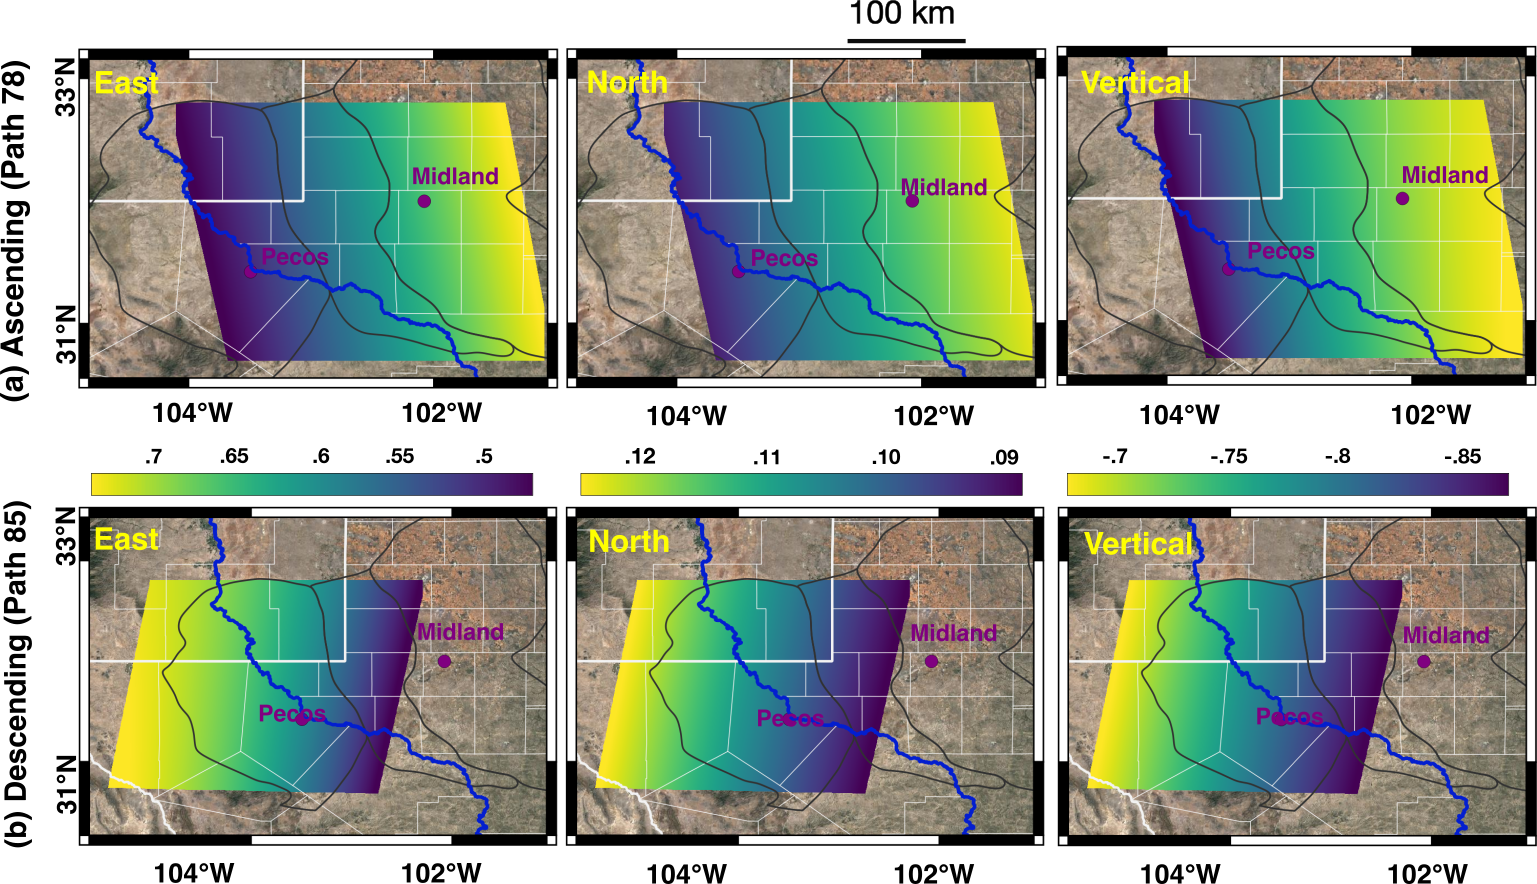
\includegraphics[width=.98\textwidth]{paper1-permian/figures/supplement/figureS2-los.pdf}
	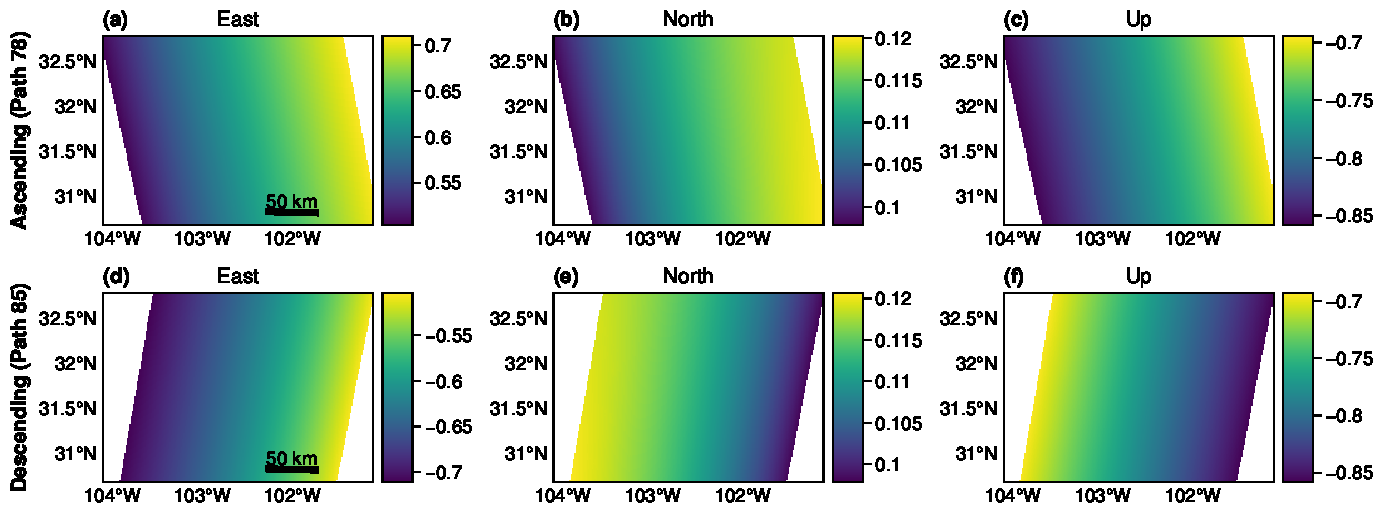
\includegraphics[width=.98\textwidth]{figures/chapter2-sar/figure_los_enu_coeffs.pdf}
	\caption[East, north, and vertical coefficients of Sentinel-1 LOS vectors]{East, north, and vertical coefficient of the LOS unit vector of all Sentinel-1 path 78 and path 85 pixels. Positive LOS direction points away from the satellite to the ground.
	}
	\label{fig:los-map}
\end{figure}

An interferogram measures surface deformation between the two SAR acquisition times along the radar line-of-sight (LOS) direction. The LOS deformation, $u_{LOS}$, can be written as: 
\begin{align}
	u_{LOS}= \alpha_{e} u_{e} + \alpha_{n} u_{n} + \alpha_{u} u_{u}
\end{align}
where $u_{e}$, $u_{n}$ and $u_{u}$ are the east, north and up displacements, respectively. The radar look vector $\alpha = [\alpha_e, \alpha_n, \alpha_u]$ can be calculated from the known imaging geometry at every pixel location. This varies significantly for Sentinel-1 due to the $ \sim$250 km wide swath (Figure \ref{fig:los-map}). 




In regions where InSAR data are available from two LOS directions, we can decompose the ground motion into its eastward and vertical components.
To perform the decomposition, we first write $u_{asc}$ and $u_{desc}$ in terms of $u_e$, $u_n$ and $u_u$:
\begin{align}
	u_{asc} &= \alpha_{a,e} u_{e} + \alpha_{a,n} u_{n} + \alpha_{a,u} u_{u}\\
	u_{desc} &= \alpha_{d,e} u_{e} + \alpha_{d,n} u_{n} + \alpha_{d,u} u_{u}
\end{align}
We can express $u_e$ and $u_u$ as:
\begin{align}
	u_{e} &\approx  \frac{1}{\beta}  \left[\alpha_{d,u}  u_{asc} - \alpha_{a,u} u_{desc} \right] \\
	u_{u} &\approx  \frac{1}{\beta}  \left[\alpha_{a,e} u_{desc} - \alpha_{d,e}  u_{asc}  \right] 
\end{align}
where  $ \beta = {\alpha_{a,e} \alpha_{d,u}- \alpha_{d,e} \alpha_{a,u}} $.




\begin{figure}
	\centering
	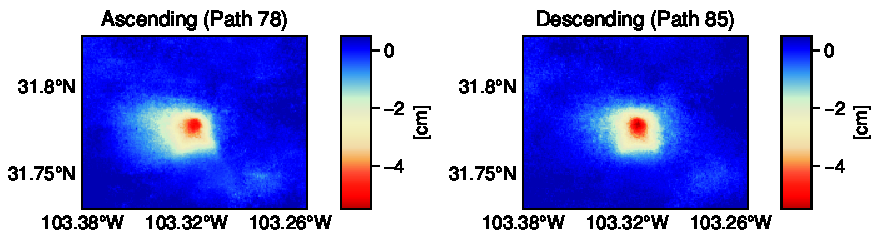
\includegraphics[width=\textwidth]{figures/chapter2-sar/injection-asc-desc.pdf}
	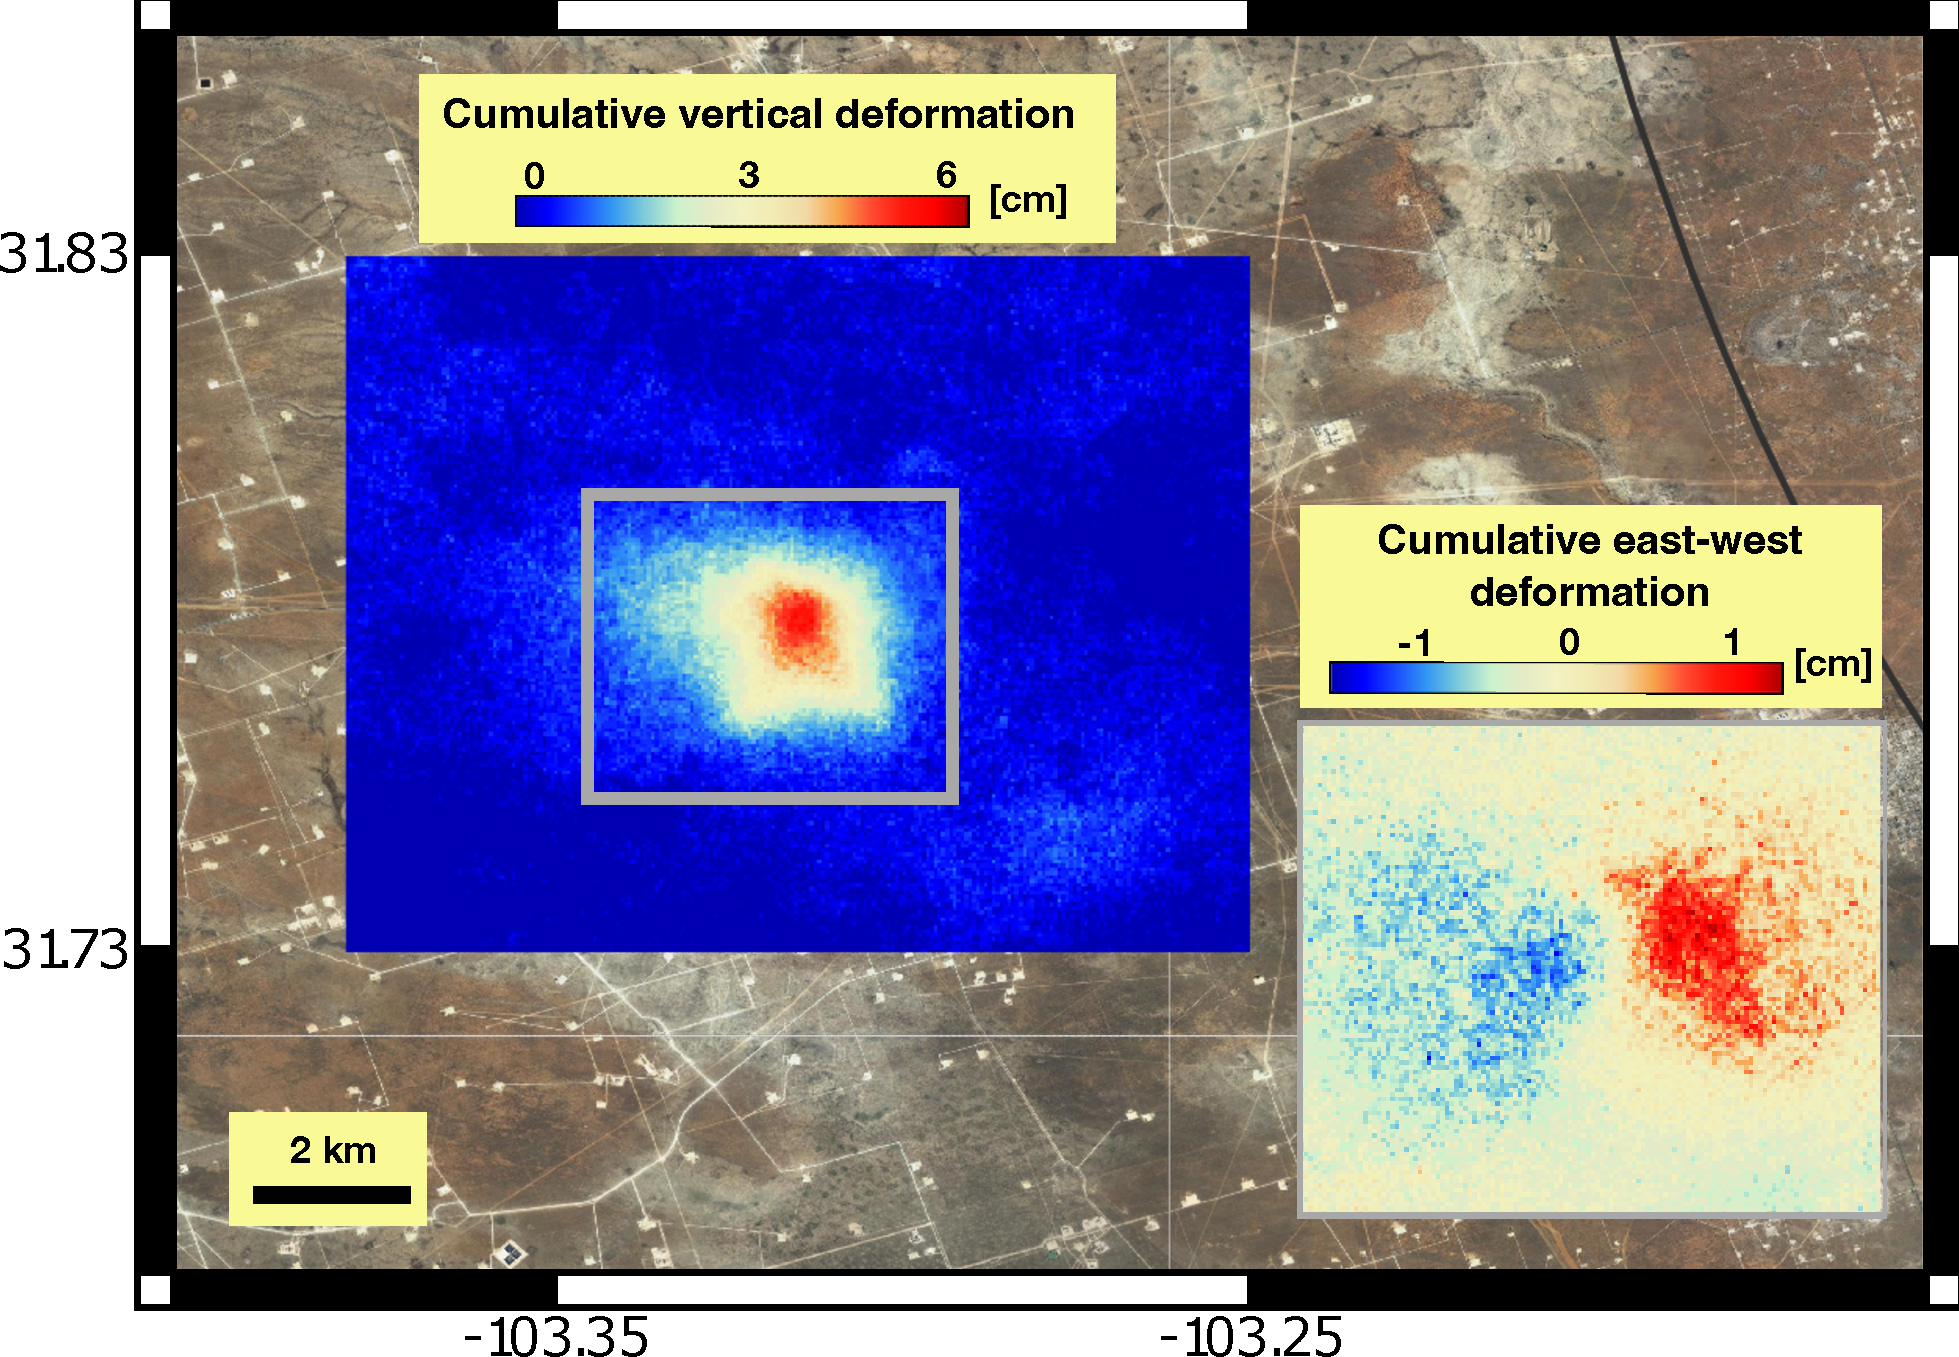
\includegraphics[width=\textwidth]{figures/chapter2-sar/injection-kim-lu}
	%	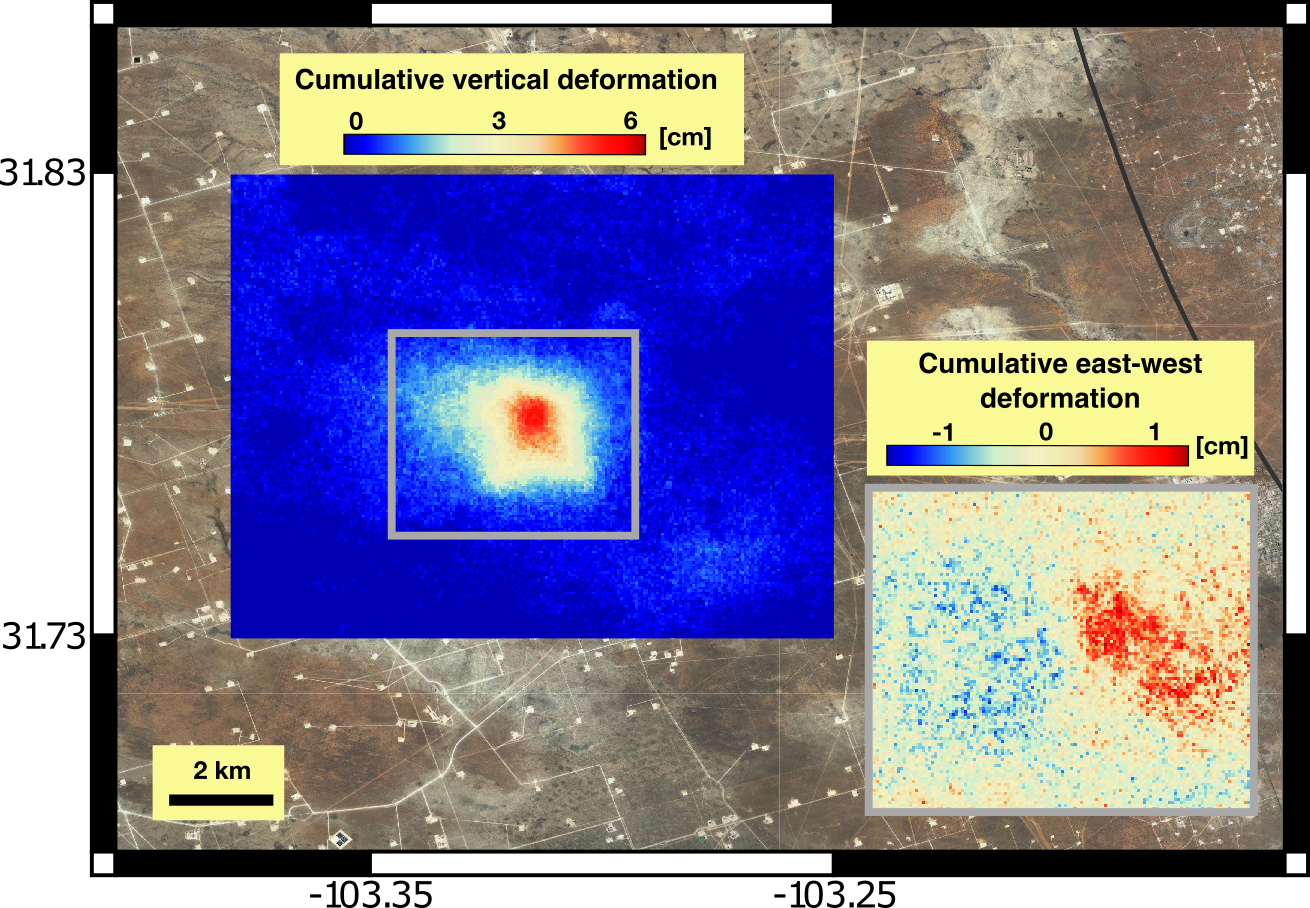
\includegraphics[width=\textwidth]{paper1-permian/figures/supplement/figureS3-injection-kim-lu.pdf}
	\caption[Vertical and horizontal deformation near Winkler County, TX]{
		(top) Ascending and descending line-of-sight cumulative deformation between November 2014 and April 2017. Red indicates motion toward each satellite.
		(bottom) Cumulative vertical and horizontal surface deformation due to wastewater injection in Winkler County, TX. The horizontal motion here is $\sim$ 20\% of the vertical motion, with up to $\sim$ 5.5 cm of uplift and $\sim$ 1.2 cm of east-west motion. This localized deformation feature was originally reported in \cite{Kim2018AssociationLocalizedGeohazards}.}
	\label{fig:ch2-injection-kim-lu}
\end{figure}



Because Sentinel-1 satellites are operating in a near-polar orbit, the north look coefficients $\alpha_{a,n}$ and $\alpha_{d,n}$ are both relatively small. Ignoring 1 cm northward motion in $u_n$ only leads to $\sim$ 0.1-0.2 mm error in $u_e$ and $\sim$ 1 mm error in $u_u$ at most locations. 

To illustrate a decomposition, Figure \ref{fig:ch2-injection-kim-lu} shows a 12 km x 12 km region centered on a wastewater injection well found by \cite{Kim2018AssociationLocalizedGeohazards} to show injection-related uplift. We observe similar magnitude deformation toward the satellite in both ascending and descending tracks (Figure \ref{fig:ch2-injection-kim-lu} top). After decomposing the two geometries using the LOS vector at each pixel, we observed $\sim$ 5.5 cm of uplift and $\sim$1.2 cm of east-west motion between November 2014 and April 2017 (Figure \ref{fig:ch2-injection-kim-lu} bottom). 

% ORIGINAL:  \cite{Kim2018AssociationLocalizedGeohazards} detected several localized deformation features within the Delaware Basin related to wastewater injection, CO2 injection, and hydrocarbon production using Sentinel-1 InSAR data.  Our LOS decomposition results are consistent with their study at these locations. For example, in a 12 km x 12 km region centered on a wastewater injection well, we observed $\sim$ 5.5 cm of uplift and $\sim$1.2 cm of east-west motion between November 2014 and April 2017 (Figure \ref{fig:injection-kim-lu}). 



%
%\subsection{Uncertainty Propagation through LOS decomposition}
%\label{sec:ch2-decomp-uq-prop}
%Since the LOS decomposition is a linear operation, given two LOS uncertainties, we can use linear uncertainty propagation theory to determine the vertical/horizontal uncertainties.
%
%TODO: move this to appendix or not?
%


\section{InSAR processing chain}
\label{sec:ch2-processing}
We developed software for an efficient and scalable InSAR processing chain to process geocoded SLC images and output cumulative surface deformation maps (Figure \ref{fig:ch2-processing}). An area of interest (AOI) is chosen in latitude and longitude coordinates, and all overlapping Sentinel-1 SLC products from a specified time frame are downloaded from the Alaska Satellite Facility (ASF) Distributed Active Archive Center (DAAC). The NASA Shuttle Radar Topography Mission (SRTM) \citep{Nasa2013NasaShuttleRadar} 30 meter DEM is downloaded for the AOI (stitching together tiles for regions larger than 1 x 1 degree) and upsampled.
The DEM, along with ESA's precise orbit files, are used by the Stanford processor \cite{Zheng2017PhaseCorrectionSingle, Zebker2017UserFriendlyInsar} to produce topography corrected, geocoded SLCs (GSLCs).
We note that working with GSLCs simplifies workflows for merging multiple Sentinel-1 frames over large areas \citep{Zheng2019ImagingCascadiaSlow}.
Interferograms are formed from the GSLCs through a pixel-wise cross multiplication (Equation \eqref{eq:ch2-conj-mult}), which are then unwrapped using the Statistical-cost, Network-flow Algorithm for Phase Unwrapping (SNAPHU) \citep{Chen2001TwoDimensionalPhase}. The unwrapped interferograms are referenced and (optionally) denoised by removing a planar or quadratic phase ramp. These are finally saved using the Hierarchical Data Format 5 (HDF5) data format, which allows user-defined metadata, data chunking, and compression.  HDF5 also simplifies and accelerates parallel implementations of pixel-wise SBAS algorithms (used in Chapter \ref{CHAP:4-GRL} and \ref{CHAP:5-robust-ts}).
%While equivalent interferograms can be produced by other software such as GMTSAR \citep{Sandwell2011OpenRadarInterferometry} or ISCE \citep{Rosen2012InsarScientificComputing}, 
% reduces the interferogram formation step to a simple cross multiplication, and they .
% as well as the ingesting future acquisitions  over the same AOI.



\begin{figure}
	\centering
	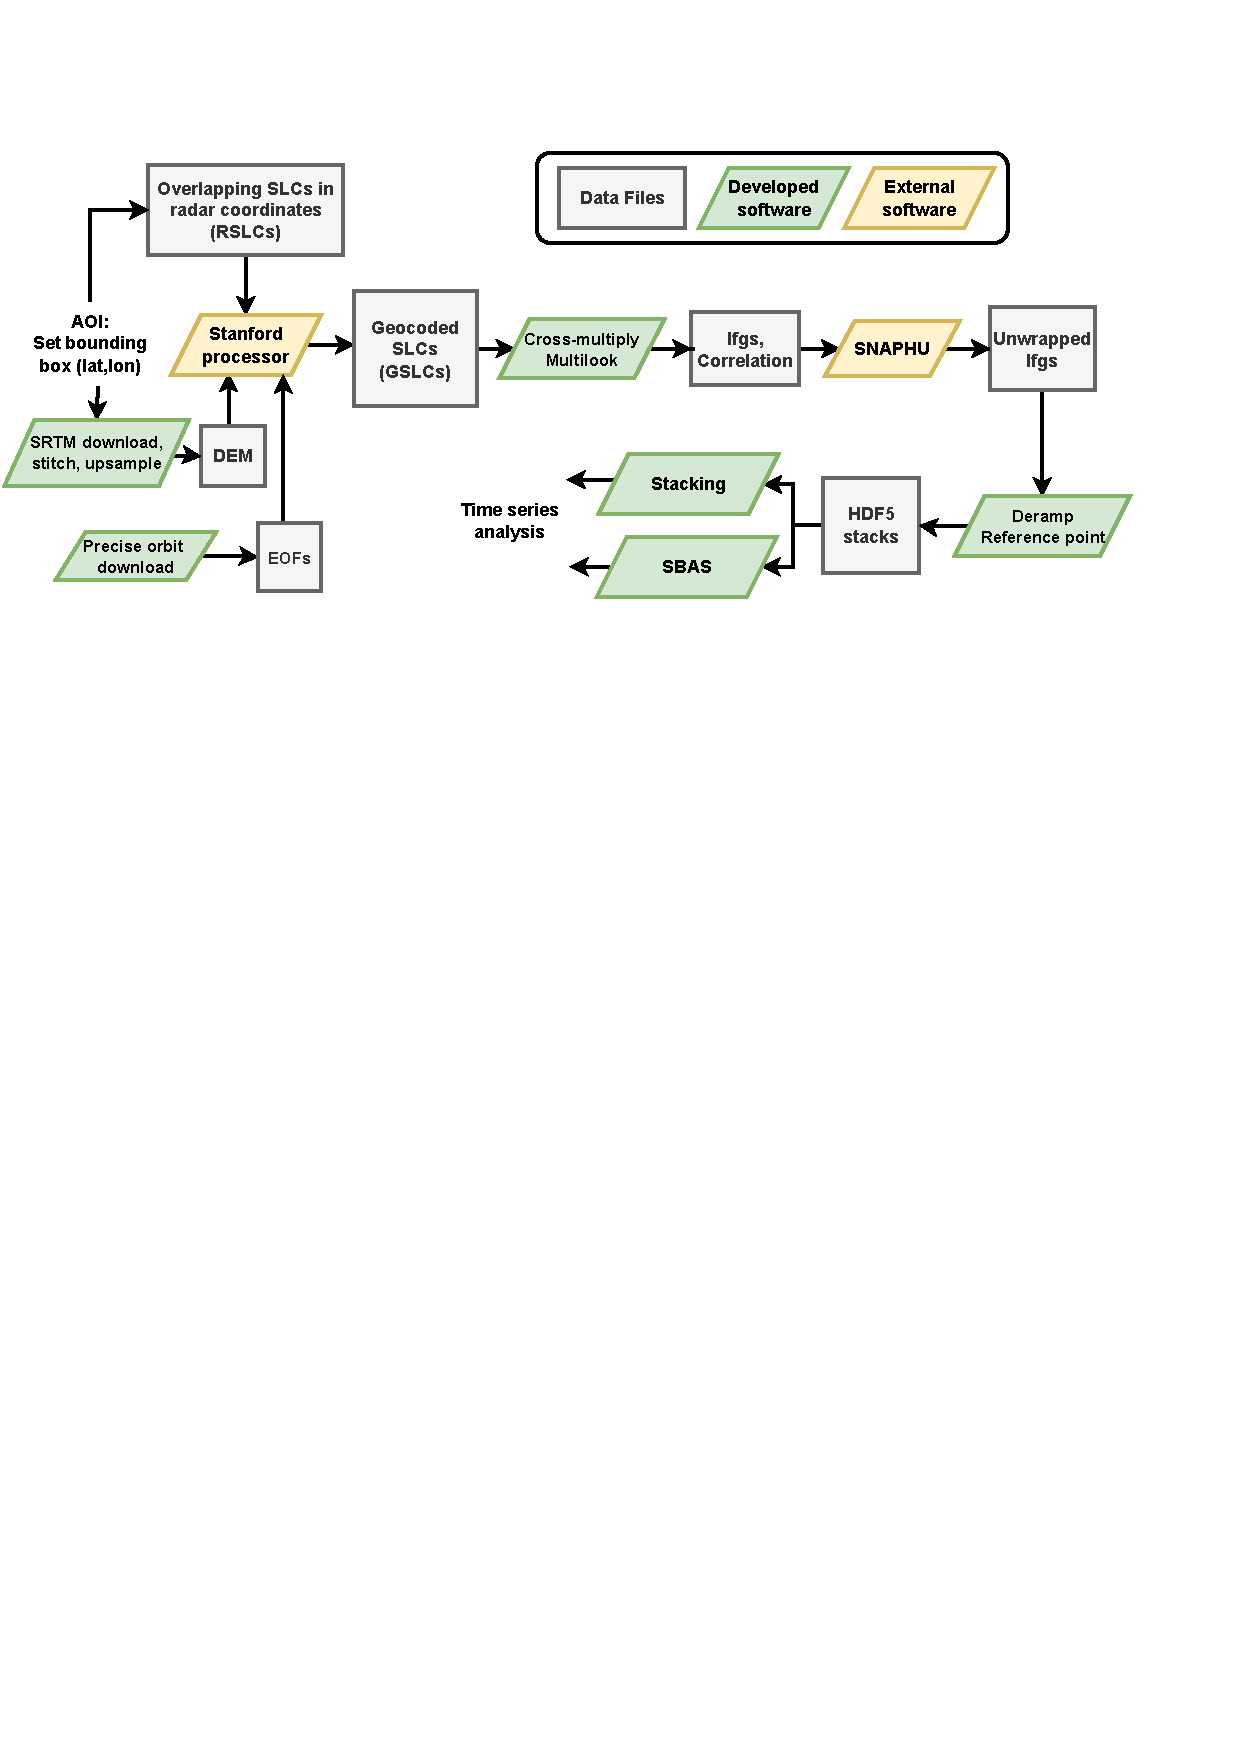
\includegraphics[width=\textwidth]{figures/chapter2-sar/processing-flow.pdf}
	\caption[Diagram of InSAR processing chain]{
	Processing chain used to create geocoded unwrapped of interferograms for stacking or SBAS time series analysis. Grey boxes indicate intermediate data products, yellow parallelograms indicate externally developed software packages, green parallelograms indicate software written for this thesis.
}
	\label{fig:ch2-processing}
\end{figure}


%- insatead of just TS formula, maybe mention the software... "geocoded SLCs". "write software into geocoded SLCs". "maybe one of the core group proc..."
%- somehow reflect that i can contribute to mintpy
%- one of key strengths... 'they can write fancy ts formula' they download software and run it... 
%- things i did aren't in mintpy... so could mention that the things will be developed for our radar interfeometry group
%- lot of people talk about algo method result... then you found they just ran code. "i ran this correction"
%- this was a reason she got hired. 



\chapter{InSAR Background}
\label{CHAP:3}

In this chapter...

%Simons: operating at microwave frequencies, synthetic aperture radar (SAR) systems provide unique images representing the electrical and geometrical proper- ties of a surface in nearly all weather conditions. Since they provide their own illumination, SARs can image in daylight or at night. 

%https://www.usgs.gov/observatories/yvo/news/insar-magic-deformation-camera-no-one-saw-coming
%Tracking radars "ping" a target, record the reflected signal, and measure (1) how long it took for the ping's round trip, and (2) the frequency of the return signal. The travel time is a measure of distance to the target. The target's velocity can be determined from the frequency of the return signal, which differs from that of the transmitted signal as a result of the Doppler effect (this is the effect that makes a siren sound different when it is coming toward you versus moving away from you, for example). Air traffic control radars and police speed detectors work on this principle.

\section{Radar Imaging}
\label{CHAP:3-radar}

``Radar'' was originally an acronym for ``RAdio Detection And Ranging'' but it has since become ubiquitous enough enter the common vernacular. Unlike passive sensors that rely on illumination for outside sources, such as optical cameras, a radar is an active sensor that emits its own electromagnetic energy. 
As such, radars are able to operate both day and night, and generally operate at microwave frequencies that are not blocked by clouds (around between 1 GHz and 300 GHz, or wavelengths of 3 m to 1 mm).
%The ability to operate both day and night is one of the main advantages of radar.

The original radars developed during World War 2 were for tracking the position of targets. In these systems, the range to the target is calculated from the round trip travel time of an electromagnetic pulse that is reflected off the target, and the angle is determined by the antenna pointing direction.
%system emits pulses of electromagnetic energy and detects the time delay of their return, which can be converted to a range using the speed of light. 
Later researchers developed imaging radar systems converted a series of radar pulses on a moving platform into a two-dimension image. Although these images originally had coarse resolution, research led by Carl Wiley at Goodyear in the 1950s resulted in the development of the radar imaging technique known as synthetic aperture radar (SAR) \citep{Wiley1954PulsedDopplerRadar, Wiley1985SyntheticApertureRadars}.
%Since electromagnetic waves get scattered by objects that are roughly the size of their wavelength, this means that radars are not blocked by water droplets and may see through clouds.
%At Goodyear in the 1950s, Carl Wiley developed the concept of the synthetic aperture \citep{Wiley1954PulsedDopplerRadar}, which was the start of the radar imaging technique known as synthetic aperture radar (SAR) \citep{Wiley1985SyntheticApertureRadars}.
The first demonstration of a spaceborne earth-observing SAR mission with interferometric capability was Seasat, launched by NASA in 1978
%equipped with an L-band radar 
\citep{Born1979SeasatMissionOverview, Gabriel1989MappingSmallElevation}.
Since that time, there have been dozens of mission launched by various space agencies, leading some to call the last decade ``the golden age of SAR'' \citep{Moreira2014GoldenAgeSpaceborne}.

%Synthetic aperture radar (SAR) is a powerful radar imaging technique which works day and night through all weather conditions.



\subsection{Timeline of SAR Constellations}



\begin{figure}
	\centering
	\includegraphics[width=1.1\textwidth]{figures/chapter3-sar/sar-missions.pdf}
	\caption[Timeline of government SAR missions]{Timeline of government-sponsored SAR missions since 1990. Bar lengths indicate life span of mission. Bars which intersect the right edge indicate ongoing missions.
		Colors indicate the space agency operating the mission.
		Missions which provide data free of charge to the general public (as of May 2022) are marked with blue stars.
		Vertical sections of the timeline are divided by the radar frequency of the sensor, showing (from top to bottom) the X-band, C-band, and L-band missions.
		Note that SIR-C/X-SAR and SRTM were equipped with both C- and X-band sensors.}
	\label{fig:ch3-sar-missions}
\end{figure}


Figure \ref{fig:ch3-sar-missions} shows a timeline of SAR missions that have been launched by governments and space agencies since 1990. The missions are grouped vertically into the three most commonly used frequency bands for SAR sensors in earth-observing missions: L-band (wavelengths of $\sim$24 cm), C-band ($\sim$6 cm cm) and X-band ($\sim$3 cm).
During the 90s, the European Space Agency (ESA) launched two C-band SAR satellites: ERS-1 in 1991 and ERS-2 in 1995. The ERS-1 satellite provided the first practical demonstration of spaceborne InSAR's ability to capture surface deformation
when \cite{Massonnet1993DisplacementFieldLanders} mapped the  surface deformationn pattern caused by the 1992 Landers, California earthquake. The first L-band SAR satellite, JERS-1, was launched by NASDA\footnote{Although JERS-1 is labeled as a JAXA mission in Figure \ref{fig:ch3-sar-missions}, it was run by NASDA at the time. In 2003, NASDA merged with two other Japanese space agencies, ISAS and NAL, to form JAXA.} in 1992, and the Canadian Space Agency (CSA) launched their own C-band mission, RADARSAT-1, in 1995.


The most influential SAR mission within the science community has been Sentinel-1 \citep{Torres2012GmesSentinel1}. First launched in 2014, the Sentinel-1 satellites acquire data using an imaging mode that allow them to image very large swaths ($\sim$240 km wide in the interferometry mode) \cite{Zan2006TopsarTerrainObservation}, allowing them revisit any point on Earth every 12 days. 
Additionally, Sentinel is the first mission of it's kind to provide it's data for free, leading to a transition from using SAR and InSAR in opportunistic experiments to being able to operationally monitor nearly anywhere on Earth  \cite{Rosen2021ShiftingGround}.
Currently Sentinel-1 is the only ongoing mission with open SAR data; however, the future launch of the NISAR ISRO SAR mission (NISAR) will also provide free L-band SAR data with global coverage \citep{Rosen2015NasaIsroSar}.


\begin{figure}
	\centering
	\includegraphics[width=1.0\textwidth]{figures/chapter3-sar/sar-private-constellations.pdf}
	\caption[Private sector SAR constellations]{SAR constellations run by private companies, showing the number of currently launched satellites (blue) stacked under the number of future planned launches (gold). Note the broken y-axis scale, as two companies 
		%	(China Electronics Technology Group and PredaSAR) 
		are planning constellations of 96 satellites.
	}
	\label{fig:ch3-sar-private-const}
\end{figure}



The first small SAR SmallSats (satellites weighing under 180 kg) have been launched by private companies over the past four years (Figure \ref{fig:ch3-sar-private-const}). Finland's ICEYE had its first succesful launch in January 2018, while Capella Space had their first launch 11 months later. Seven other companies have since launched at least 1 SAR satellite, and in the next five years, there are plans to launch over 500 additional SAR SmallSats \citep{Kulu2021SatelliteConstellations2021}. While many large SAR constellations expect sub-hourly revisit time for any given point on earth \citep{Stringham2019CapellaXband}, only the large government SAR missions, such as Sentinel-1, ALOS, and NISAR, explicitly plan for consistent global coverage in their mission objectives. However, the possibility of daily or hourly InSAR revisit times opens many new applications previously not possible with the 6-12 day revisit times of large SAR missions \citep{YagueMartinez2021TowardsFrequentFlood, Taylor2021RemoteSensingMountain, Kitajima2021PotentialSarSmall}.






\section{Synthetic Aperture Radar}
\label{CHAP:3-sar}


Synthetic aperture radar is an imaging technique that uses a pulsed radar mounted on a moving platform. A two-dimensional image is created by coherently processing the returned energy pulses. While the images are often displayed in grayscale and may appear similar to optical images, they represent the electrical and geometrical properties of the objects in the scene \cite{Simons2007InterferometricSyntheticAperture}.
%To create a radar image, the energy scattered by points on the ground must be collected and focused in two dimensions.  The image represents the electrical and geometrical properties of the scene \cite{Simons2007InterferometricSyntheticAperture} 


The SAR imaging geometry is shown in Figure \ref{fig:ch3-sar-geometry}. A side-looking radar on a platform at height $h$ moves in the azimuth directory $x$ at a velocity $v$.  The radar repeatedly emits pulses at some interval (called the \emph{pulse repetition interval}, or PRI) that travel in the range direction.
%The illuminated portion of the ground has a swath width of $r \lambda / w$
%The width of the swath for stripmap operation is controlled by the antenna width, $w$, as $r \lambda / w$. Likewise, the size of the illuminated swath in the along track direction is $r \lambda / L$.
The line of sight (LOS) vector is defined as the unit vector pointing from the radar antenna to a point in the illuminated ground swath.
Each pulses illuminates a portion of the ground, known as the radar footprint.


\begin{figure}
	\centering
		\includegraphics[width=0.99\linewidth]{figures/chapter3-sar/ch3-sar-geometry.pdf}
	\caption[Acquisition geometry of an imaging radar]{Acquisition geometry of an  imaging radar. A platform containing a radar instrument is moving with speed $v$ in the azimuth/along-track direction, $x$ at a height $h$.
    The slant range $r$ to the ground point is measured along the line-of-sight (LOS) direction from the antenna to the ground.
   	The radar antenna here has length $L$ (in the azimuth direction) and width $w$.
   	As the radar sends out pulses, each one into an area on the ground called the beam ``footprint'' (oval shape). 
%   	As the platform moves and sends more pulses, they sweep out the radar swath (gray region).
	}
	\label{fig:ch3-sar-geometry}
\end{figure}

% Resolution: shorter pulse better resolution, but also lowers SNR. To get around tradeoff, send long with LFM chip to high snr and fine resolution in range direction
%

The signal to noise ratio (SNR) of the system depends on the total energy transmitted.  SNR can be increased by either sending a higher peak power (which is often limited by design constraints) or sending a pulse of longer duration $\tau$. This presents a dilemma: sending pulses with a larger $\tau$ results in coarser range resolution $\delta_r$, where resolution is the ability to distinguish scatters illuminated by the same radar pulse. In the absence further processing, the resolution in range would is $\delta_r = \frac{c \tau}{2}$, where $c \approx 3 \times 10^8$ is the speed of light. Thus, a pulse with $\tau = 30 $ microseconds would have about a 4.5 km resolution.

However, SAR systems usually transmit pulsed waveforms called \emph{chirps} whose frequency $f$ increases over time. For example, in a linear frequency moduled (LFM) chirp, the frequency can be written as 
\begin{equation}
	f(t) = k t
\end{equation}
where $k$ is the chirp slope (in Hz / s) and $-\tau / 2 < t < \tau/2$.
These special waveforms allow the receiver to correlate the returned echoes with a \emph{matched filter}, or a replica of the transmitted chirp. The new range resolution after using the matched filter depends on the frequency bandwidth, $BW$, of the chirp:  $BW = f_{max} - f_{min}$.
improves the range resolution to $\delta_r = \frac{c}{2 BW}$, where is the frequency bandwidth of the chirp. 


Figure \ref{fig:ch3-range-compress} demonstrates the effect of using chirped waveforms on range resolution using an example chirp with parameters matching the ERS-1 satellite (Figure \ref{fig:ch3-range-compress}a).
%The real part of an example chirp with parameters matching the ERS-1 satellite has an oscillation frequency which increases linearly over time (Figure \ref{fig:ch3-range-compress}a). 
The chirp has a duration of $\tau \approx 37.12 \mu s$, a chirp slope $k$ of $4 \times 10^{11} Hz / s$, resulting in frequency bandwidth $BW = k \tau$ $\approx$15.5 MHz (Figure \ref{fig:ch3-range-compress}b). By correlating the transmitted chirp with its complex conjugate, we get the impulse response of a point scatter (Figure \ref{fig:ch3-range-compress}c). If a chirp with the same time duration had a smaller slope $k$ (Figure \ref{fig:ch3-range-compress}d), the bandwidth would shrink by the same proportion (Figure \ref{fig:ch3-range-compress}e), and the impulse response would also be more spread out (Figure \ref{fig:ch3-range-compress}f).
Thus, we see that using chirped waveforms reverses the original problem, as a pulse with larger bandwidth actually has better resolution than a shorter pulse.


\begin{figure}
	\centering
%	\includegraphics[width=0.99\linewidth]{figures/chapter3-sar/ch3-range-compress.pdf}
	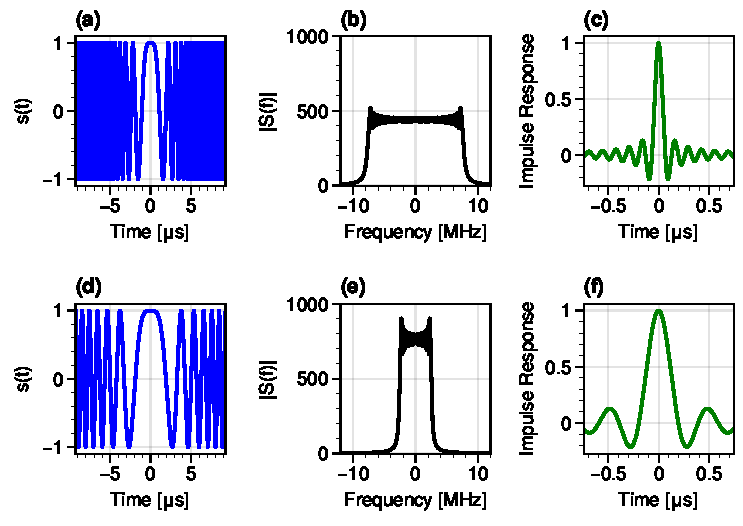
\includegraphics[width=0.99\linewidth]{figures/chapter3-sar/radar-chirp-bandwidth-ers.pdf}
%		\includegraphics[width=0.99\linewidth]{figures/chapter3-sar/radar-chirp-bandwidth-ers2.pdf}
	\caption[Range resolution from chirp compression]{
		(a) The real part of a linear frequency-modulated chirp with a duration of $\tau \approx 37.12 \mu s$ and a chirp slope $k = 4 \times 10^{11} Hz / s$.
		(b) The magnitude of the Fourier transform of the chirp is approximately a rectangle function, which shows the chirp bandwidth $BW = k \tau$ $\approx 15.5$ MHz.
		(c) Matched filtering of the returned echo from one point scatterer yields the impulse response, which shows the approximate 10 meters of range resolution (or $\sim$65 ns in time).
		(d) For a chirp with the same slope $k$ and 1/3 the duration $\tau$ the frequency bandwidth is also cut by 1/3 (e), the corresponding impulse response (f) and range resolution is 3 times worse.
	}
	\label{fig:ch3-range-compress}
\end{figure}


In the azimuth direction, the size of the radar footprint determines which ground points can be distinguished from the echo of one pulse;  this is known as the \emph{real aperture radar} (RAR) resolution. The footprint size can be written as $r \lambda / L$, which comes from the antenna's angular beam width of $\lambda / L$ and the range $r$ to the target. The earliest radar imaging platforms were limited to this resolution in azimuth. For an airborne platform with a 1 meter antenna imaging at C-band, this would be a $\sim$600 meter resolution. Note that for some applications, such as military detection applications or wide-area ocean mapping \cite{Simons2007InterferometricSyntheticAperture}, this azimuth resolution is sufficient; however, the RAR resolution for spaceborne radars are on the order of 10s of kilometers, which is far too coarse for most applications.


%The advantages long wavelengths offer in terms of penetration come with compensating drawbacks. The resolution a sensor depends on the wavelength and on the size of its aperture—the mirror or lens in the case of a camera or a telescope, the antenna in a radar. If you lengthen the wavelength, you increase the size of the aperture you need in order to achieve a given resolution. To produce detailed images with radar requires a very large aperture indeed—far larger than anything a single spacecraft can offer.

%> Synthetic-aperture radar (SAR) provides a way round that problem. Satellites move at quite a clip—typically, in low orbit, around 25,000kph. By taking all the echoes a radar satellite gets from a given target as it passes over it—and processing them into a single image, SAR produces a result as precise as if it had been made using a single aperture as wide across as the distance the satellite travelled while gathering the data—tens of hundreds of kilometres (see diagram).
The resolution in azimuth can be greatly improved by creating a \emph{synthetic aperture}, which is a technique that processes the reflected echoes coherently (i.e. using both magnitude and phase) to focus the image (Figure \ref{fig:ch3-synth-aper}).
%where the energy from a series of pulse returns from a point target is coherently added.
Coherent processing is possible by carefully tracking each target's phase history, $ \phi(t) $, which is related to the range to the target $r(t)$ by $\phi(t) = -\frac{4 \pi}{\lambda} r(t)$.
There are multiple image formation algorithms which create this synthetic aperture and use the phase history. One of the first developed and most widely today used is the range-Doppler algorithm (RDA) \citep{Wu1976DigitalSystemProduce, Cumming1979DigitalProcessingSeasat}. 
RDA uses the apparent shift in Doppler frequency due to the platform motion to create a matched filter in azimuth, similar to the matched filter used for range compression.
%RDA is a frequency-domain algorithm, since it converts the phase history 
%Which converts the range-compressed data into the frequency domain. 
An alternative to RDA is time-domain backprojection \citep{Duersch2013BackprojectionSyntheticAperture}, which provides a more exact phase compensation at the cost of being more computationally expensive.
The backproject algorithm collects the energy from every radar pulse containing a pixel after compensating for the range-dependent phase.
The complex-valued radar image $I$ for the pixel at location $ (x, y) $ can be formed by summing over all pulses:
\begin{equation}
	I(x, y) = \sum_{k} s(r(x, y, k)) \exp[-j \frac{4 \pi}{\lambda} r(x, y, k)]
\end{equation}
where $r(x, y, k)$ is the range distance from the radar sensor to the point $ (x, y) $ at the time of the $k$th pulse, and $s(r)$ is the value of the returned pulse at the given range \citep{Zebker2018InsarMissionLevel}.
Thus, if the radar imaging geometry is known precisely, the coherent summation can be performed to focus the SAR image and achieve a final azimuth resolution of
%Processing all echoes coherently results in a fine resolution in the azimuth direction, which is equal to the resulting that would be attainable only by a real aperture of length $2 L_s$ \citep{Cumming2004DigitalProcessingSynthetic}.
%The phase of each return echo at a time $t$ is related to the range $r$ by $\phi(t) = -\frac{4 \pi}{\lambda} r(t)$.
\begin{equation}
	\delta_{az} = \frac{L}{2}
\end{equation}
The intuition behind this surprising result is that, unlike with RAR, a smaller physical antenna size $L$ leads to a wider beam width $\lambda / L$. This means means the same target is illuminated for a longer time and has more pulses to coherently process. Thus, the azimuth resolution will actually improve with a smaller antenna length.

\begin{figure}
	\centering
	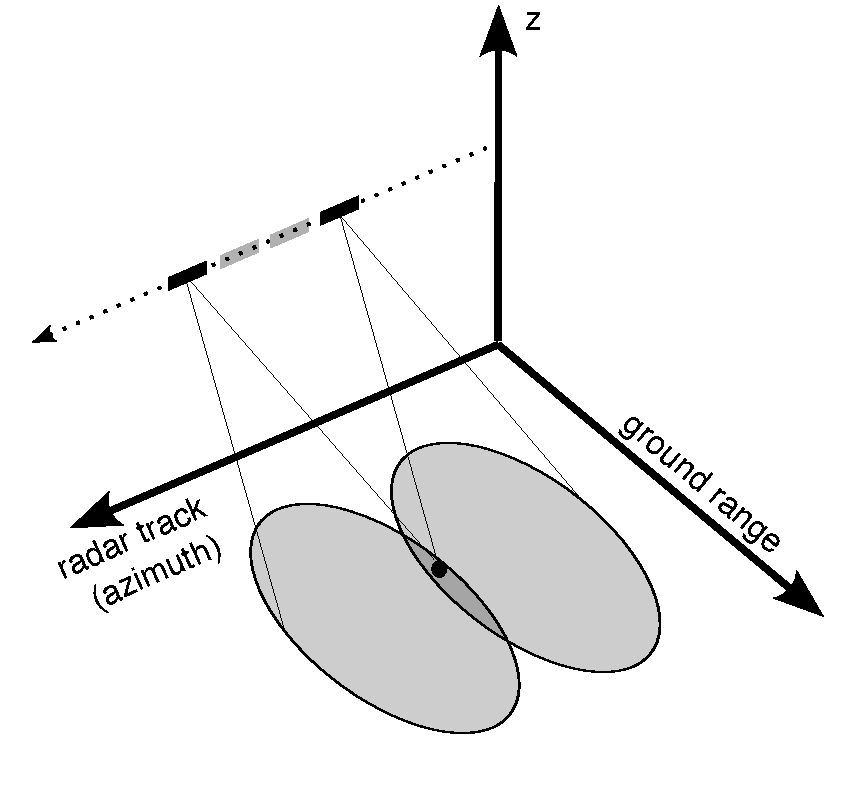
\includegraphics[width=0.8\linewidth]{figures/chapter3-sar/ch3-synth-aper2.pdf}
	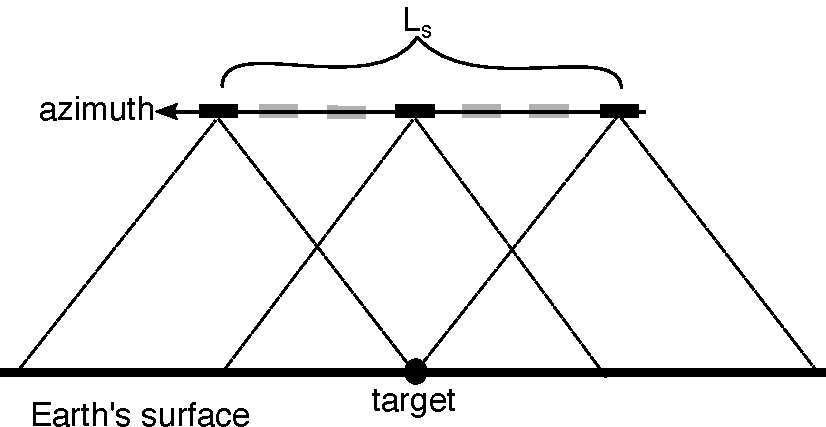
\includegraphics[width=0.99\linewidth]{figures/chapter3-sar/ch3-sar-synthetic-aperture.pdf}
	\caption[Concept of the synthetic aperture ]{Concept of the synthetic aperture.
	(Top) One point on the ground is illuminated by a series of pulses. Pictured here are the footprints of the first and last pulses that illuminate the point. 
	(Bottom) Side view of the pulses illuminating the target, forming a synthetic aperture of length $L_s$.
	}
	\label{fig:ch3-synth-aper}
\end{figure}



\section{InSAR Principles}


Possible ways to introduce phase:

- Do the InSAR geometry, get phase measure has diff of 2 phases.
- Fringe frequency, but measure "flat earth", subtract that, leads to topography.
%−2πa + φflat + φtopo + noises

OR
- ...


\begin{figure}[hbt!]
	\centering
	% TODO
	%	\includegraphics[width=0.99\linewidth]{figures/ch3-sar-geometry.pdf}
	\caption{InSAR imaging geometry for topography or deformation mapping.
	}
	\label{fig:ch3-insar-geometry}
\end{figure}




\section{InSAR Noise Sources}
\label{sec:ch3-noise}

The phase of an interferogram can be written as

\citep{Zebker1992DecorrelationInterferometricRadar, Zebker1994AccuracyTopographicMaps, Zebker1997AtmosphericEffectsInterferometric}
\begin{equation}
	\Delta \phi = \frac{4 \pi}{\lambda} \Delta d_{LOS} +  \Delta \phi_{orb} + \Delta \phi_{decor} + \Delta \phi_{unwrap}  + \Delta \phi_{dem} + \Delta \phi_{iono} + \Delta \phi_{tropo}  + \Delta \phi_{n}
\end{equation}
where $ \lambda $ is the radar wavelength and $ \Delta d_{LOS} $ is the surface deformation along the radar LOS direction. The noise terms include orbital errors, phase decorrelation, unwrapping errors, DEM inaccuracies, ionospheric and tropospheric artifacts, and other residual noise terms that are typically an order of magnitude smaller than the error terms listed here.


\subsection{Anatomy of an Interferogram}

While high signal to noise ratio (SNR) interferograms can be analyzed by simply ``counting the fringes'', as is the case for the first published Landers earthquake \cite{Massonnet1993DisplacementFieldLanders}, this is often the exception, rather than the rule.
In many cases, a single interferogram will contain more visual noise features than signals, making it difficult for a non-expert InSAR user to interpret. 

Hawaii example




\begin{figure}[!htbp]
	\centering
	\includegraphics[width=1.0\textwidth]{figures/chapter3-sar/hawaii-example.pdf}
	\caption[Sentinel-1 interferogram over Hawaii showing common noise sources, along with 2018 eruption deformation]{
		(a) Sentinel-1 interferogram from April 20th, 2018 to May 2nd, 2018 over Hawaii, spanning the beginning of the 2018 eruption event.
		Each colored phase cycle of $2\pi$ radians indicates a range change of 2.7 cm along the radar line-of-sight, which can be caused by real surface deformation or a noise source.
		(b) The dense fringes near the coast are caused by turbulent tropospheric noise (see Section \ref{sec:ch3-noise-tropo-strat}).
		(c) Stratified tropospheric noise on the peak of Mauna Kea, the tallest peak on Hawaii at 4,207 m, causes a concentric ring pattern. This pattern is also visible on Mauna Loa in the center of the island, where the phase is strongly correlated with topographic height. See Section \ref{sec:ch3-noise-tropo-strat} for further details.
		(d) An example of decorrelation noise caused by dense tropical rain forests (e) located on windward side of the island.
		(f) Real deformation of $ \sim 40 $cm around the Pu'u '\=O'\=o volcanic cone to the east of K'\=ilauea. In this case, the ground was subsiding down and to the southeast as magma flowed away from Pu'u '\=O'\=o.
		%		The signal of interest in this interferograms, the collapse of the Pu'u '\=O'\=o caldera
		(g) An aerial photo of Pu'u '\=O'\=o shows the caldera collapse on April, 30th, 2018 after magma migrated eastward underground (image source: HVO / USGS).
	}
	\label{fig:sar-hawaii-example}
\end{figure}

Two days after the interferogram on May 4, a  M$_w$ 6.9 earthquake struck the south flank of the Lower East Rift Zone, just south of the zoom.


% at the Sentinel-1  The windward side of the island contains many dense tropical rain forests. These areas show Heavy decorrelation noise at the Sentinel-1 C-band wavelength of 5.5 cm.

%brief fissure eruption occurred on the west flank of the Puʻu ʻŌʻō cone on April 30, 20181. Over the next few days, earthquakes migrated eastward into the LERZ and rift-normal displacements were recorded by GPS instruments, signaling large-scale injection of magma downrift of Puʻu ʻŌʻō. Magma reached the surface in Leilani Estates subdivision on May 3, marking the onset of the LERZ eruption (Fig. 1a)

%1. Table: noise, specific to ifg or SAR, max variance?, common?


%2. Figure: Hawaii, showing Stratified, Turbulence, decorr, defo


%3. ? Figure: unwrap error? DEM error? iono noise? orb ramp?

\subsection{Tropospheric Noise}
\label{sec:ch3-noise-tropo}

%Ideas:
%
%- comparison of ways people have tried to correct for troposphere
%
%- plots/images of possible views into the single day atmosphere.
% -- modis
% -- HRRR, ECMWF
% --  GOES
% -- insar averaging
% 
% axes of comparison:
% - resolution
% - time availability
% - spatial availibility
% - sensitivity to phase propation delay
% 
% 
% SEASONAL plots...
% 

\subsubsection{Turbulent Tropospheric Noise}
\label{sec:ch3-noise-tropo-turb}

\subsubsection{Stratified Tropospheric Noise}
\label{sec:ch3-noise-tropo-strat}


Tropospheric noise in InSAR consists of a stratified component, which correlates with topography \citep{Doin2009CorrectionsStratifiedTropospheric}, and a turbulent component that is random at time scales longer than a day \citep{Emardson2003NeutralAtmosphericDelay, Onn2006ModelingWaterVapor}. Previous studies have made advances in correcting for the stratified component using global atmospheric models \citep{Doin2009CorrectionsStratifiedTropospheric, Jolivet2014ImprovingInsarGeodesy, Cao2021AdvancedInsarTropospheric}, GPS zenith delay measurements \citep{Onn2006ModelingWaterVapor}, external measurements from sensors such as the Moderate Resolution Imaging Spectroradiometer (MODIS) \citep{Li2005InterferometricSyntheticAperture, Barnhart2013CharacterizingEstimatingNoise} or the Medium Resolution Imaging Spectrometer (MERIS)  \citep{Ding2008AtmosphericEffectsInsar}, as well as empirical methods using regressions on InSAR phase and elevation \citep{Zebker2021AccuracyModelFree, Murray2021ClusterBasedEmpirical}.

Early efforts to correct or mitigate the turbulent atmospheric noise used a combination of high pass temporal filtering and low pass spatial filtering \citep{Ferretti2001PermanentScatterersSar, Berardino2002NewAlgorithmSurface}.
%- but as \citep{Liu2012SatelliteRadarInterferometry} notes, gaps in the acquistion, or strong non-Gaussianity from, e.g., severe thunderstorms, break the assumptions of equal variance among APS dates that these filters require.
Several research efforts have attempted to produce estimates of the atmospheric phase delay for each SAR acquisition directly from a time series of interferograms. \citep{Liu2012SatelliteRadarInterferometry} formulated the problem as a linear system using a network of small baseline interferograms. Since the problem of estimating both surface deformation and atmospheric delay is an ill-posed problem given only differential InSAR measurements, the authors assumed zero or known deformation of the study region, and they constrained the estimated troposphere to have zero mean. In an attempt to denoise time series of surface deformation, \citep{Tymofyeyeva2015MitigationAtmosphericPhase} averaged sets of redundant interferograms containing a common reference date, with an assumption of linear or slowly-varying deformation, and subtracted the estimated troposphere.

%  \citep{Havazli2021DetectionThresholdEstimates} almost does what i'm doing (with some type of stratified atmo too), it's just a random multiplier, and it looks like it was almost all simulation
An alternative approach to correcting for the tropospheric turbulence is to treat it as a stochastic noise source in time series analysis \citep{Simons2007InterferometricSyntheticAperture, Agram2015NoiseModelInsar} and estimate its covariance matrix either through auxiliary data sources \citep{Barnhart2013CharacterizingEstimatingNoise, Parker2015SystematicAssessmentAtmospheric} or directly from InSAR data \citep{Lohman2005SomeThoughtsUse}. While these approaches provide a measure of uncertainty in the deformation solution, the uncertainties are given for each pixel (or each model parameter), rather than for each visible deformation feature.




GACOS is an iterative tropospheric decomposition model that integrates global weather models and available GPS zenith delay measurements for estimating tropospheric noise in InSAR data \citep{Yu2018InterferometricSyntheticAperture}. Due to the limited spatial and temporal resolution of weather models and GPS data, GACOS is more effective in removing the stratified tropospheric noise \citep{Doin2009CorrectionsStratifiedTropospheric} than the random turbulent tropospheric noise \citep{Emardson2003NeutralAtmosphericDelay}. 
We found that GACOS does not produce substantial corrections in most Sentinel-1 West Texas interferograms for areas outside the main area of interest (e.g. Figure \ref{fig:GACOS} (a)-(c)). 

\textcolor{red}{Get an interferogram that works, and then show the one that doesn't}

\begin{figure}
	\centering
	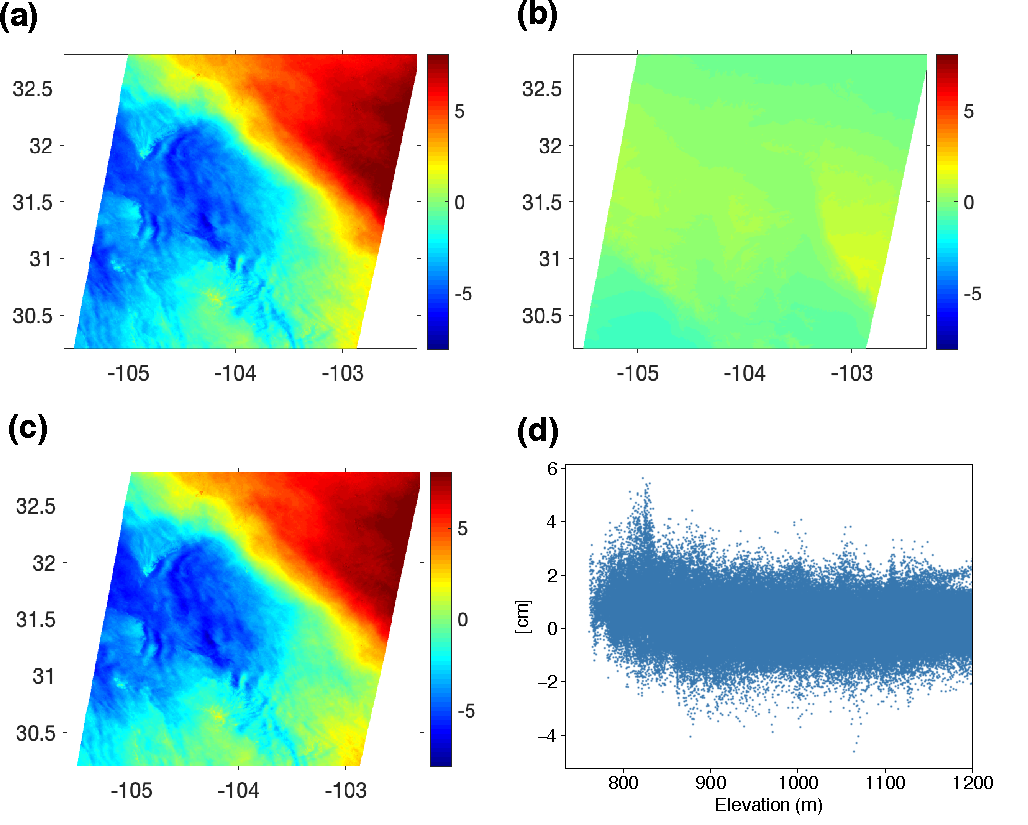
\includegraphics[width=\textwidth]{paper1-permian/figures/supplement/figureS4-gacos.pdf}		
	\caption[GACOS tropospheric corrections]{(a) LOS measurements (in cm) of a descending interferogram (20150127-20150220) before the GACOS correction. (b) GACOS tropospheric correction (in cm) for the 20150127-20150220 interferogram \citep{Yu2018InterferometricSyntheticAperture}. (c) LOS measurements (in cm) of a descending interferogram (20150127 - 20150220) after the GACOS correction. (d) LOS measurements (in cm) of the 20150127-20150220 interferogram vs. the Digital Elevation Model (DEM).}
	\label{fig:GACOS}
\end{figure}


\section{InSAR Time Series}
\label{sec:ch3-insar-ts}

stacking for avg rate

SBAS linear system. doesn't need to be short baseline. just a way to solve for the phase at each date

Phase linking approaches solve for this using an optimization on each pixels time-covariance matrix.


% Yunjun thesis: the vector of interferometric phase residual that does not fulfill the zero phase closure of interferogram triplets. It includes the decorrelation noise, phase contribution due to the change of dielectric properties of ground scatterers such as soil moisture (De Zan et al., 2014; Morrison et al., 2011), processing inconsistency such as filtering, multilooking, coregistration and interpolation errors (Agram and Simons, 2015; Hanssen, 2001), and/or phase-unwrapping errors.

%An alternative objective function to solve equation (2.1) is minimizing the L2-norm of the residual of phase velocity of adjacent acquisitions (equation (16) in Berardino et al. (2002)). Optimizations with both objective functions give nearly identical solutions for a fully connected network


\subsection{Uncertainty}
\label{sec:ch3-eq-tropo}
Several ways for uncertainty.

jackknife (maybe look into the NSBAS/GIANT time series way they do it....). prob an underestimate, since this is *precision* of the estimator. often it's jsut precision of the noise+deformation phase. but we really want the defo phase.

other is least squares propagation of covariance. difficult to calibrate without good atmo noise estimate, can underestimate/overestimate.

one problem with daily time series: often uncertainty is a single number. but each day's atmo noise can vary by 10-20x.

Even with temporal smoothing (example pic of that super storm cell), there can be many days with "blobs" of atmospheric noise which exceed real deformation.

Chapter (2nd paper) will discus a third novel way using computer vision.


Bootstrap:

From "practictioners guide":
A natural question for the practitioner is to ask  “ Why bootstrap in the linear regression case? Isn ’ t least - squares a well - established approach that  has  served  us  well  in  countless  applications? ”   The  answer  is  that  for  many  problems, least - squares regression has served us well and is always useful as  a first approach but is problematic when the residuals have heavy - tailed distributions or if even just a few outliers are present.

IID assumption: doesn't hold for time series... still gives some estimate. maybe show example of how it overestimates, but that it's not bad because it's mostly accounting for tropo, and not for the phase UQ (cite Zwiebeck paper).


%Problems with pixelwise
%- Image of blob, with 8 mm cutoff, question which part you trust and not
%- Leads into feature-wise uq



\section{InSAR Line-of-sight Decomposition}
\label{sec:ch3-insar-decomp}
An interferogram measures surface deformation between the two SAR acquisition times along the radar line-of-sight (LOS) direction. The LOS deformation, $u_{LOS}$, can be written as: 
\begin{align}
	u_{LOS}= \alpha_{e} u_{e} + \alpha_{n} u_{n} + \alpha_{u} u_{u}
\end{align}
where $u_{e}$, $u_{n}$ and $u_{u}$ are the east, north and up displacements, respectively. The radar look vector $\alpha = [\alpha_e, \alpha_n, \alpha_u]$ can be calculated from the known imaging geometry at every pixel location. This varies significantly across the basin due to the $ \sim$250 km wide Sentinel swath (Figure \ref{fig:los-map}). 


%
%\begin{figure}
%	\centering
%	% TODO
%	%	\includegraphics[width=\textwidth]{}
%	\caption[Line of sight convention]{Line of sight convention used in this thesis for ascending (a) and descending (b) satellite geometries. Vector points from the satellite to the ground}
%	\label{fig:los-asc-desc}
%\end{figure}

\begin{figure}[!htbp]
	\centering
	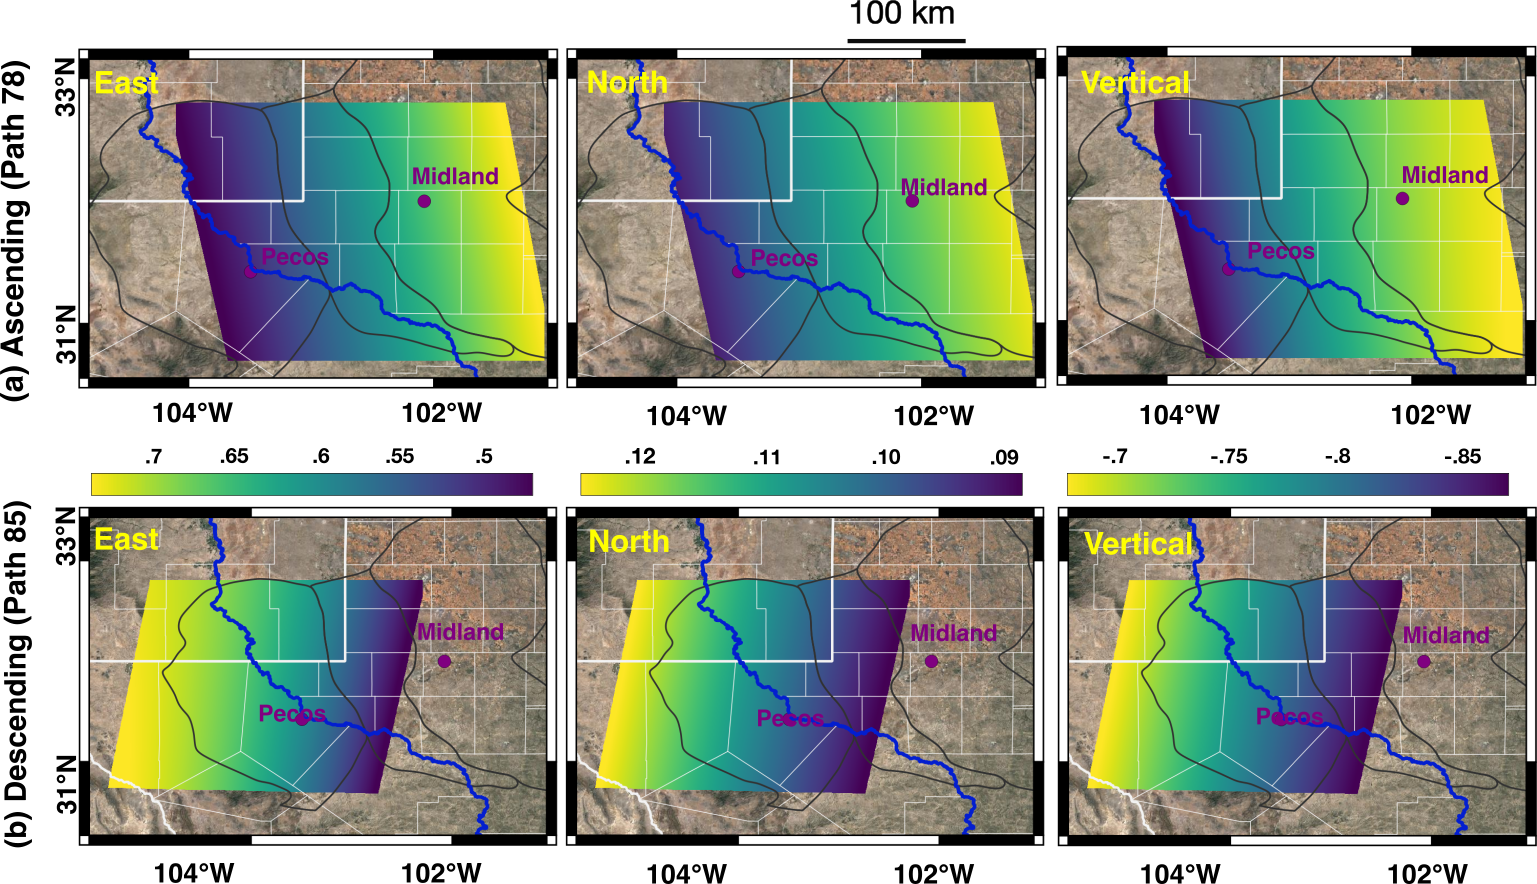
\includegraphics[width=.98\textwidth]{paper1-permian/figures/supplement/figureS2-los.pdf}
	\caption[East, north, and vertical coefficients of Sentinel-1 LOS vectors]{East, north, and vertical coefficients of the LOS unit vector of all Sentinel-1 path 78 and path 85 pixels. Positive LOS direction points away from the satellite to the ground.}
	\label{fig:los-map}
\end{figure}

In regions where InSAR data are available from two LOS directions, we can decompose the ground motion into its eastward and vertical components.
To perform the decomposition, we first write $u_{asc}$ and $u_{desc}$ in terms of $u_e$, $u_n$ and $u_u$:
\begin{align}
	u_{asc} &= \alpha_{a,e} u_{e} + \alpha_{a,n} u_{n} + \alpha_{a,u} u_{u}\\
	u_{desc} &= \alpha_{d,e} u_{e} + \alpha_{d,n} u_{n} + \alpha_{d,u} u_{u}
\end{align}
We can express $u_e$ and $u_u$ as:
\begin{align}
	u_{e} &\approx  \frac{1}{\beta}  \left[\alpha_{d,u}  u_{asc} - \alpha_{a,u} u_{desc} \right] \\
	u_{u} &\approx  \frac{1}{\beta}  \left[\alpha_{a,e} u_{desc} - \alpha_{d,e}  u_{asc}  \right] 
\end{align}
where  $ \beta = {\alpha_{a,e} \alpha_{d,u}- \alpha_{d,e} \alpha_{a,u}} $.

Because Sentinel-1 satellites are operating in a near-polar orbit, the north look coefficients $\alpha_{a,n}$ and $\alpha_{d,n}$ are both relatively small. Ignoring 1 cm northward motion in $u_n$ only leads to $\sim$ 0.1-0.2 mm error in $u_e$ and $\sim$ 1 mm error in $u_u$ at most locations. \cite{Kim2018AssociationLocalizedGeohazards} detected several localized deformation features within the Delaware Basin related to wastewater injection, CO2 injection, and hydrocarbon production using Sentinel-1 InSAR data.  Our LOS decomposition results are consistent with their study at these locations. For example, in a 12 km x 12 km region centered on a wastewater injection well, we observed $\sim$ 5.5 cm of uplift and $\sim$1.2 cm of east-west motion between November 2014 and April 2017 (Figure \ref{fig:injection-kim-lu}). 



\begin{figure}
	\centering
	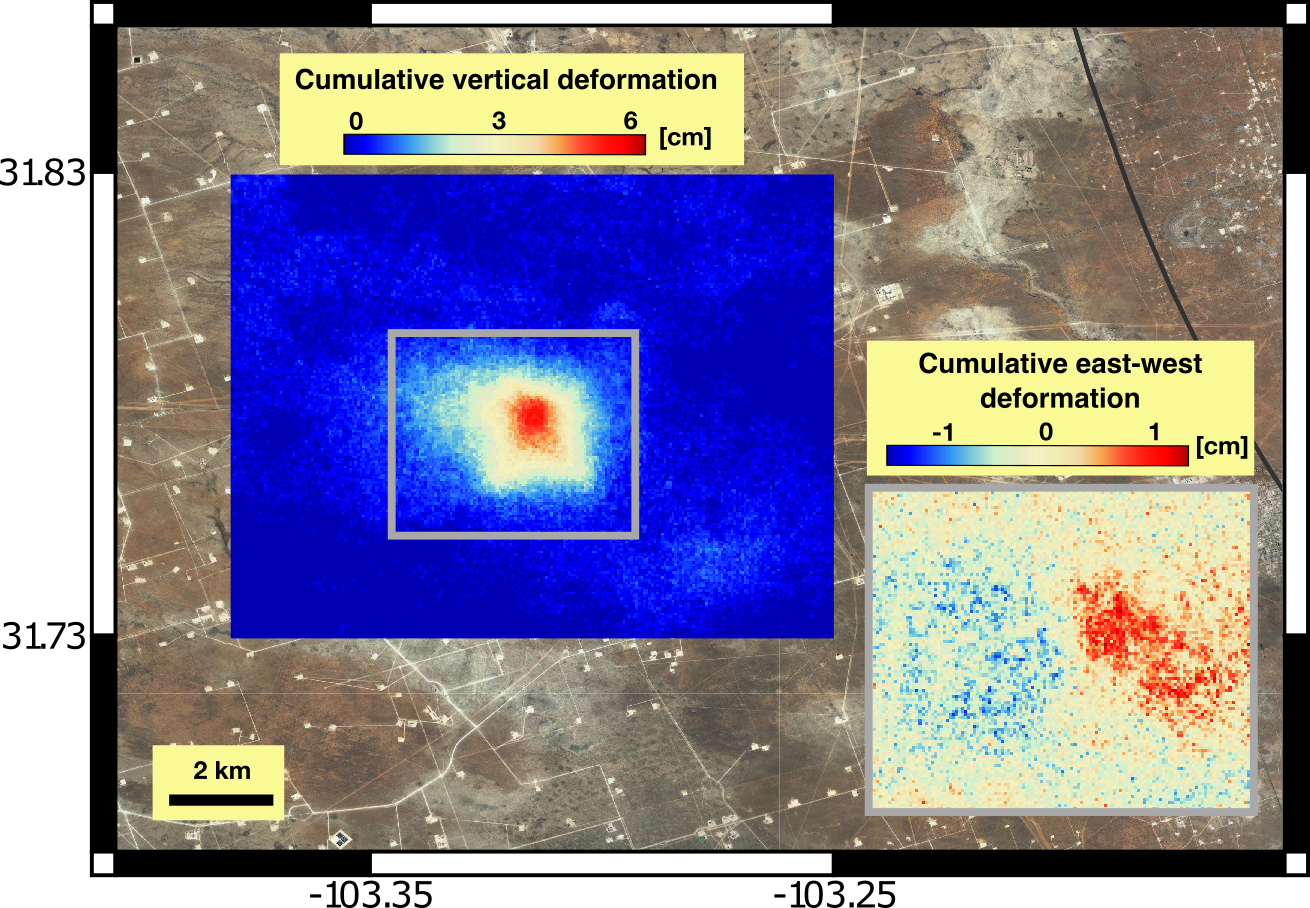
\includegraphics[width=\textwidth]{paper1-permian/figures/supplement/figureS3-injection-kim-lu.pdf}
	\caption[Vertical and horizontal deformation near Winkler County, TX]{Cumulative surface deformation between November 2014 and April 2017 due to wastewater injection in Winkler County, TX. The horizontal motion here is $\sim$ 20\% of the vertical motion, with up to $\sim$ 5.5 cm of uplift and $\sim$ 1.2 cm of east-west motion. This localized deformation feature was originally reported in \cite{Kim2018AssociationLocalizedGeohazards}.}
	\label{fig:injection-kim-lu}
\end{figure}




\subsection{Uncertainty Propagation through LOS decomposition}
\label{sec:ch3-decomp-uq-prop}
Since the LOS decomposition is a linear operation, given two LOS uncertainties, we can use linear uncertainty propagation theory to determine the vertical/horizontal uncertainties.

TODO: move this to appendix or not?





\chapter{Cumulative Surface Deformation over the Permian Basin with Automated Outlier Removal}
\label{CHAP:4-GRL}

%In this chapter,  we present a simple yet effective time series method for creating cumulative surface deformation maps over large regions with severe tropospheric noise. We use the method to create yearly deformation maps over the oil-producing region of the Permian Basin. The method incorporates an automated outlier detection and removal algorithm, which enabled ~2 mm/year agreement with GPS measurements in the presence of $\sim$15 cm of tropospheric noise.


Previous InSAR studies have demonstrated the utility of surface deformation data for understanding causes of induced seismicity; however, these studies focused on study areas $ \sim $ 60-by-60 km or smaller. 
%Basin-wide InSAR surface deformation data with detailed uncertainty quantification are needed for assessing the likelihood of induced seismicity risk in the Permian Basin. 
Since InSAR tropospheric noise variance increases with the distance away from the reference point, it is difficult to expand the InSAR spatial coverage to the entire Permian Basin while retaining millimeter level accuracy.  
In this chapter, we present a time series method for creating large cumulative surface deformation maps over areas containing severe tropospheric noise. 
We developed an outlier detection algorithm that removes InSAR measurements corrupted by severe tropospheric noise (e.g. storms and heat waves).
% withing multiple subsets of interferograms and produces a linear velocity estimate for each subset.
The method reduces the uncertainty in our linear deformation estimates by a factor of 2, down to 1-3 mm/year across the basin. Our results were validated by independent GPS measurements recorded at 13 permanent ground stations. 
We use the method to create yearly deformation maps from November 2014 through January 2019 over the oil-producing region of the Permian Basin, which are available through the Center for Integrated Seismicity Research (CISR) for the broader scientific community. 



%Within Texas, \cite{Shirzaei2016SurfaceUpliftTime} reported indications of surface uplift due to wastewater injection near a 2012 M4.8 earthquake, though limited validation for the ALOS data was available at this site near Timpson, TX \citep{Semple2017IncompleteInventorySuspected}. \cite{Kim2018AssociationLocalizedGeohazards} detected multiple deformation bowls within the Delaware Basin related to wastewater injection, $CO_2$ injection, and hydrocarbon production using Sentinel-1 InSAR data. \cite{Zheng2019WastewaterLeakageWest} incorporated InSAR-derived surface deformation data into a poroelastic model to analyze the geomechanical processes near an uplift signal in northern West Texas. They discovered that the observed surface deformation was likely caused by injection well leakages, rather than pressure increases at the planned injection depth, and the leaks may have contributed to freshwater contamination. More recently, \cite{Deng2020SurfaceDeformationInduced} used ascending Sentinel-1 LOS measurements to infer pore pressure change and Coulomb failure stress change at three sites in the southern Delaware Basin. They suggested that certain groups of earthquakes are likely induced by fluid injection, but noted that local rock structure and media properties are key controls on the area's susceptibility to induced seismicity.

%Previous InSAR studies demonstrated the use of InSAR surface deformation data for understanding causes of induced seismicity; however, these studies only focused on study areas $ \sim $ 60-by-60km or smaller, and basin-wide InSAR surface deformation data with detailed uncertainty quantification are needed for assessing the likelihood of induced seismicity risk. Since InSAR tropospheric noise variance increases with the distance away from the reference point \citep{Emardson2003NeutralAtmosphericDelay}, it is difficult to expand the InSAR spatial coverage to the entire Permian basin while retaining millimeter level accuracy. 

%In this chapter, we show that the increasing quantity and quality of Sentinel-1 SAR data allows us to average thousands of interferograms and mitigate strong tropospheric noise. We developed an outlier detection algorithm that removes InSAR measurements corrupted by severe tropospheric noise (e.g. storms and heat waves) and reduces InSAR measurement uncertainty by another factor of 2, down to 1-3 mm/year across the basin. Our results were validated by independent GPS measurements recorded at 13 permanent ground stations. 
%The InSAR-observed subsidence patterns over the Pecos area can be modeled as dip-slip over multiple normal faults and discretized cylindrical reservoir compaction. 
%Our InSAR deformation maps are now available through the Center for Integrated Seismicity Research (CISR) for the broader scientific community. 
%This dataset, when combined with physics-based reservoir and fault modeling, can produce insights into the causes of induced seismicity. 
%Furthermore, these surface deformation data products can be used to assess the areal effectiveness of the oil and gas production, a measure for estimating which regions of a reservoir are being depleted most quickly. InSAR techniques now provide a low-cost method to assist oil and gas operations and risk management at a basin-scale.

\section{Algorithms}


\subsection{Stacking and InSAR time series analysis}
\label{sec:ch4-method-compare}
%[Method only, define equations and formulas. This already outlines how we solve for deformation]

To investigate how InSAR measurement noise influences the LOS deformation solutions, we compared the results derived from (1) the stacking method, (2) an SBAS linear deformation (constant velocity) model with $L_1$ and $L_2$-norm penalty functions, and (3) unregularized and regularized SBAS deformation time series. 
We assume there are $M$ small-baseline interferograms that were generated from $N$ SAR scenes acquired over a period of interest. 
%The stacking method from \cite{Sandwell1998PhaseGradientApproach} solves for the average velocity over the study period. 
%An interferogram measures surface deformation that occurred between the two SAR acquisition times along the radar line-of-sight (LOS) direction \citep{Hanssen2001RadarInterferometryData}.
We employed a stacking approach \citep{Sandwell1998PhaseGradientApproach} to calculate the average LOS velocity $v_{avg}$ of each ground pixel over a time period of interest $T$ as:
\begin{equation}
	v_{avg} = \frac{\sum_{i \in G} \bm{\Delta  d}_i}{\sum_{i \in G} \bm{\Delta t}_i}
	\label{eq:ch4-stacking}
\end{equation}
where $G$ is a subset of interferograms that were formed using two SAR scenes acquired within the time period $T$. The LOS measurement (in cm) and the temporal baseline of the $i^{th}$ interferogram in $G$ are written as $  \bm{\Delta  d_i} $ and $ \bm{\Delta t}_i $ respectively. 
%In Section \ref{sec:ch4-method-compare}, we show that comparable LOS velocity estimates can be produced using the Small Baseline Subset (SBAS) approach \citep{Berardino2002NewAlgorithmSurface} with a constant velocity (linear deformation) model.


Similarly, the SBAS method outlined in Section \ref{sec:ch2-insar-ts} can be augmented with a linear deformation model.
In this formulation, we solve for the average velocity $ v_{avg} $ over this period at each pixel of interest as \citep{Berardino2002NewAlgorithmSurface}:
\begin{equation}
	\arg \min_{v_{avg}} \norm{ \bm{BP} v_{avg} - \bm{\Delta d}   }_p
	\label{eq:ch4-sbas-linear}
\end{equation}
where $ \bm{B }$ is the $ M \times (N-1) $ SBAS matrix, $ \bm{P}$ is an $ (N-1) \times 1 $ vector of ones, $ \bm{\Delta d} $ is the $ M \times 1 $ vector of LOS measurements (in cm) at this pixel, and $ p \in \{1, 2\} $ is the norm used to penalize the data misfit. The $L_2$ linear deformation solution is comparable to the stacking solution (with an assumption of a constant velocity), and the $L_1$ solution is typically less sensitive to measurement outliers than the $L_2$ solution.

The LOS surface velocities between adjacent SAR acquisitions $ \bm{v} = \left[v_1 , \ldots , v_{N-1} \right]^T $ can be solved as:
\begin{equation}
	\arg \min_{\bm{v} } \norm{ \bm{Bv} - \bm{\Delta d}   }^2_2 + \alpha \norm{ \bm{Dv} }^2_2  \label{eq:ch4-sbas}
\end{equation}
where $ \bm{D} $ is a $ (N-2) \times (N-1) $ matrix, with $1$ on the main diagonal and $-1$ on the superdiagonal, which approximates the first-order differentiation operator. The first term penalizes the data misfit, the second term is a temporal smoothness constraint, and $ \alpha \in \mathbb{R} $ is the weight between the two terms. When $ \alpha = 0 $, the solution is the unregularized SBAS deformation time series. An additional integration of $\mathbf{v}$ over time yields the LOS deformation time series.




%%An interferogram measures surface deformation that occurred between the two SAR acquisition times along the radar line-of-sight (LOS) direction \citep{Hanssen2001RadarInterferometryData}.
%We employed a stacking approach \citep{Sandwell1998PhaseGradientApproach} to calculate the average LOS velocity $v_{avg}$ of each ground pixel over a time period of interest $T$ as:
%\begin{equation}
%	v_{avg} = \frac{\sum_{i \in G} \Delta  d_i}{\sum_{i \in G} \Delta t_i}
%	\label{eq:ch4-stacking}
%\end{equation}
%where $G$ is a subset of interferograms that were formed using two SAR scenes acquired within the time period $T$. The LOS measurement (in cm) and the temporal baseline of the $i^{th}$ interferogram in $G$ are written as $\Delta d_i$ and $ \Delta t_i $ respectively. In Section \ref{sec:ch4-method-compare}, we show that comparable LOS velocity estimates can be produced using the Small Baseline Subset (SBAS) approach \citep{Berardino2002NewAlgorithmSurface} with a constant velocity (linear deformation) model.

%
%\section{Study site and data}
%\label{sec:ch4-site}


\subsection{Tropospheric noise outlier removal}
\label{sec:ch4-outlier-method}

We examined interferograms at the 13 control locations and discovered that non-Gaussian tails (outliers) are present. For example, LOS measurements of the ascending interferograms at pixels near the GPS station TXMC show a near zero median (-4 mm) and a standard deviation of 3.2 cm (Figure \ref{fig:ch4-outliers} (a)). Due to the absence of substantial deformation signal at this station, the standard deviation of the LOS distribution is a measure of turbulent tropospheric noise.  We found that the median LOS turbulent error is close to zero (no systematic noise bias) at all GPS control stations. The standard deviation of the turbulent noise increases as the square root of the distance from the InSAR reference point (Figure \ref{fig:ch4-outliers} (b)). Furthermore, we compared the LOS turbulent noise distribution observed at each GPS station to a normal distribution using a normal probability plot \citep{Filliben1975ProbabilityPlotCorrelation}. We discovered that non-Gaussian tails (outliers) are present (e.g. Figure \ref{fig:ch4-outliers}(c)) as a result of severe tropospheric noise (e.g. storms or heat waves). 



\begin{figure}
	\centering
	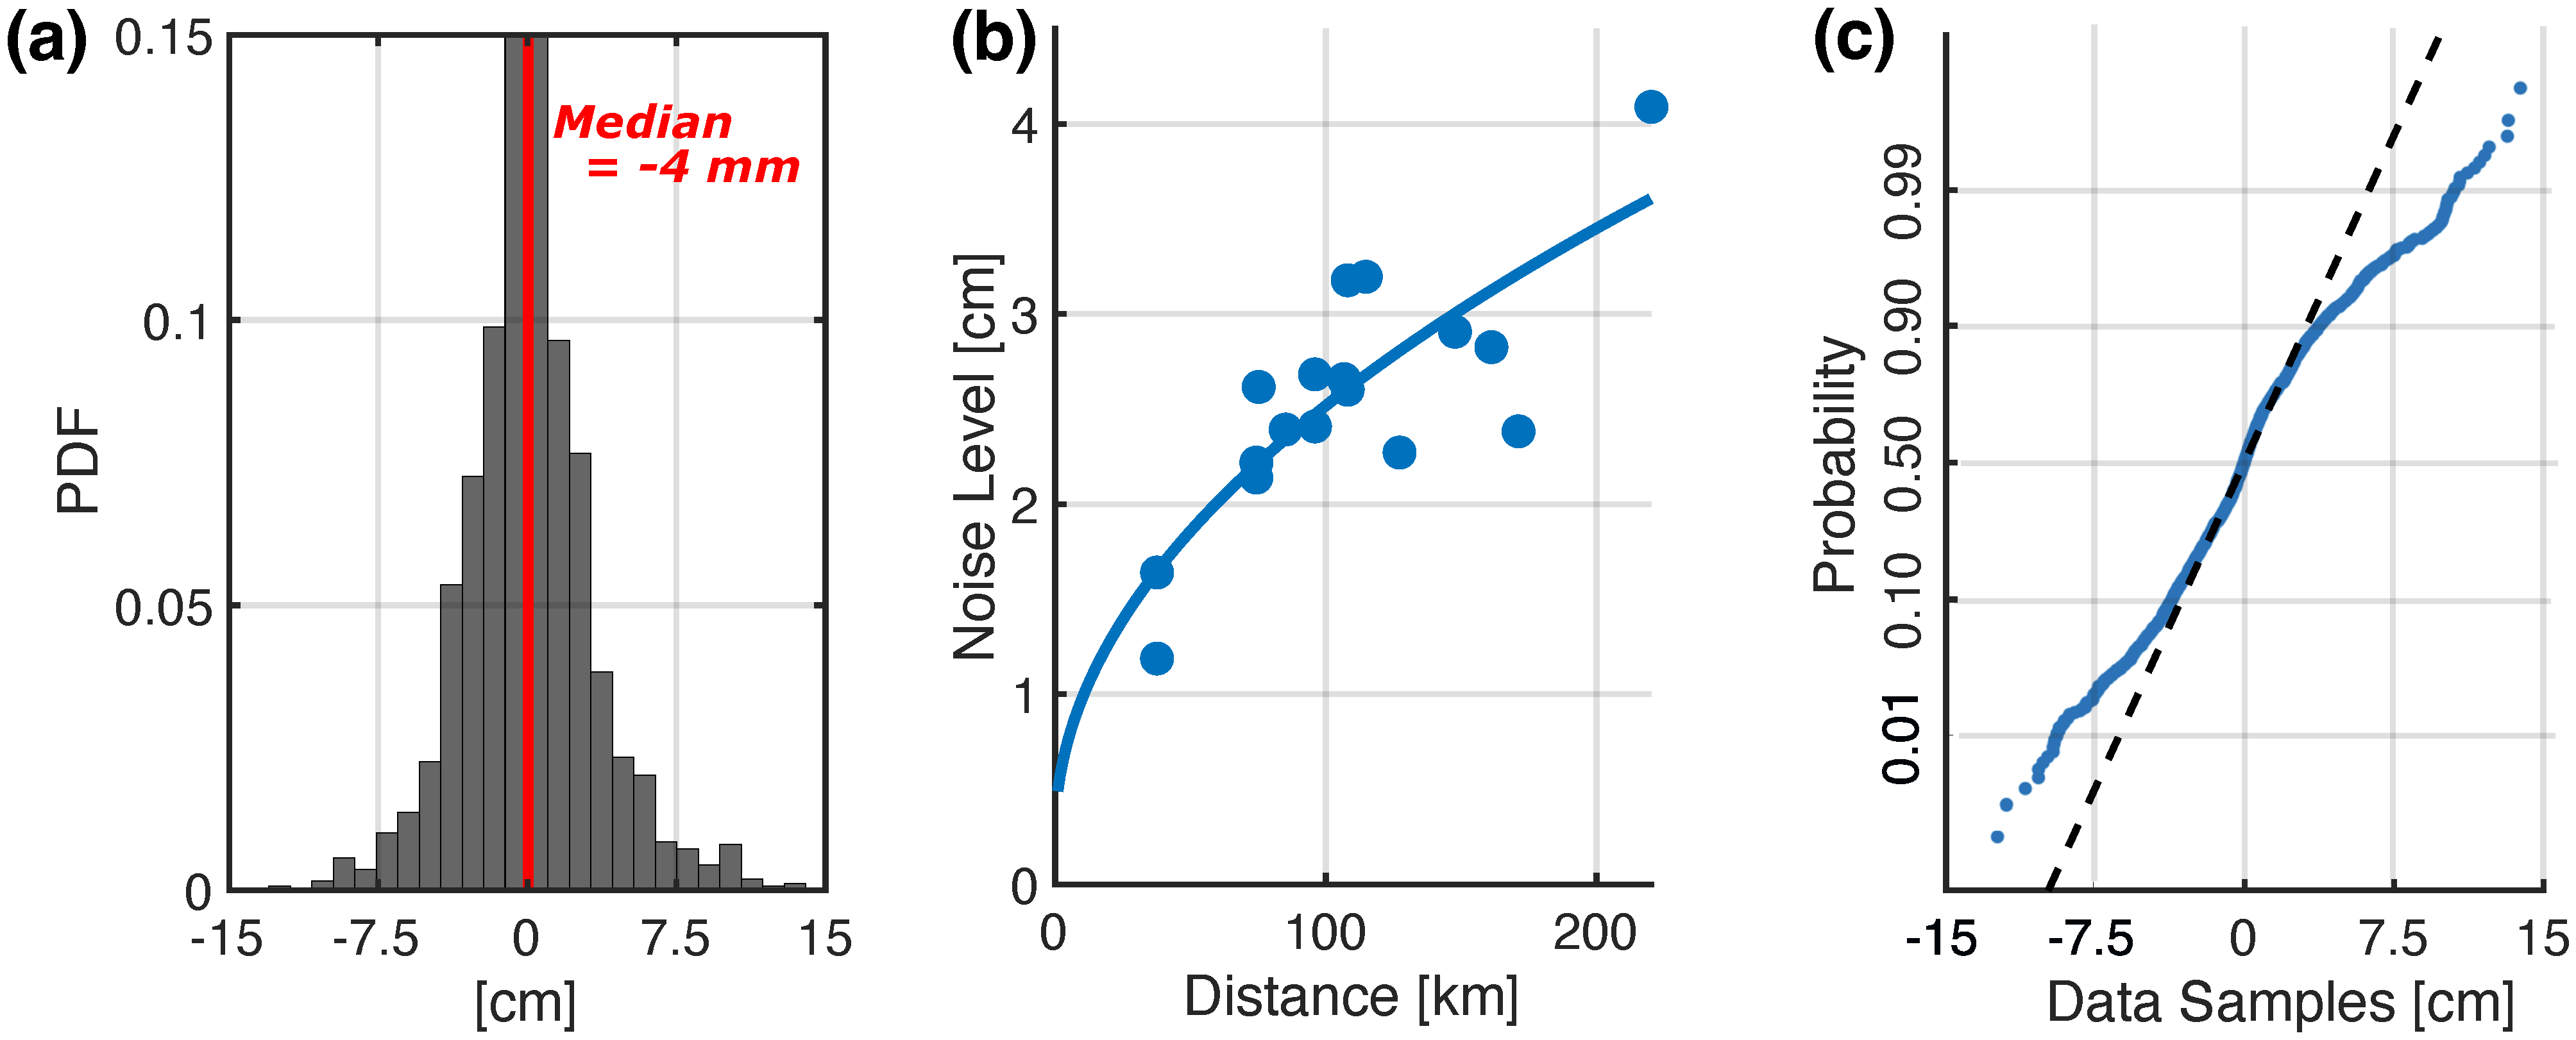
\includegraphics[width=0.99\linewidth]{figures/chapter4-grl/outlier-top-only.pdf}
	%	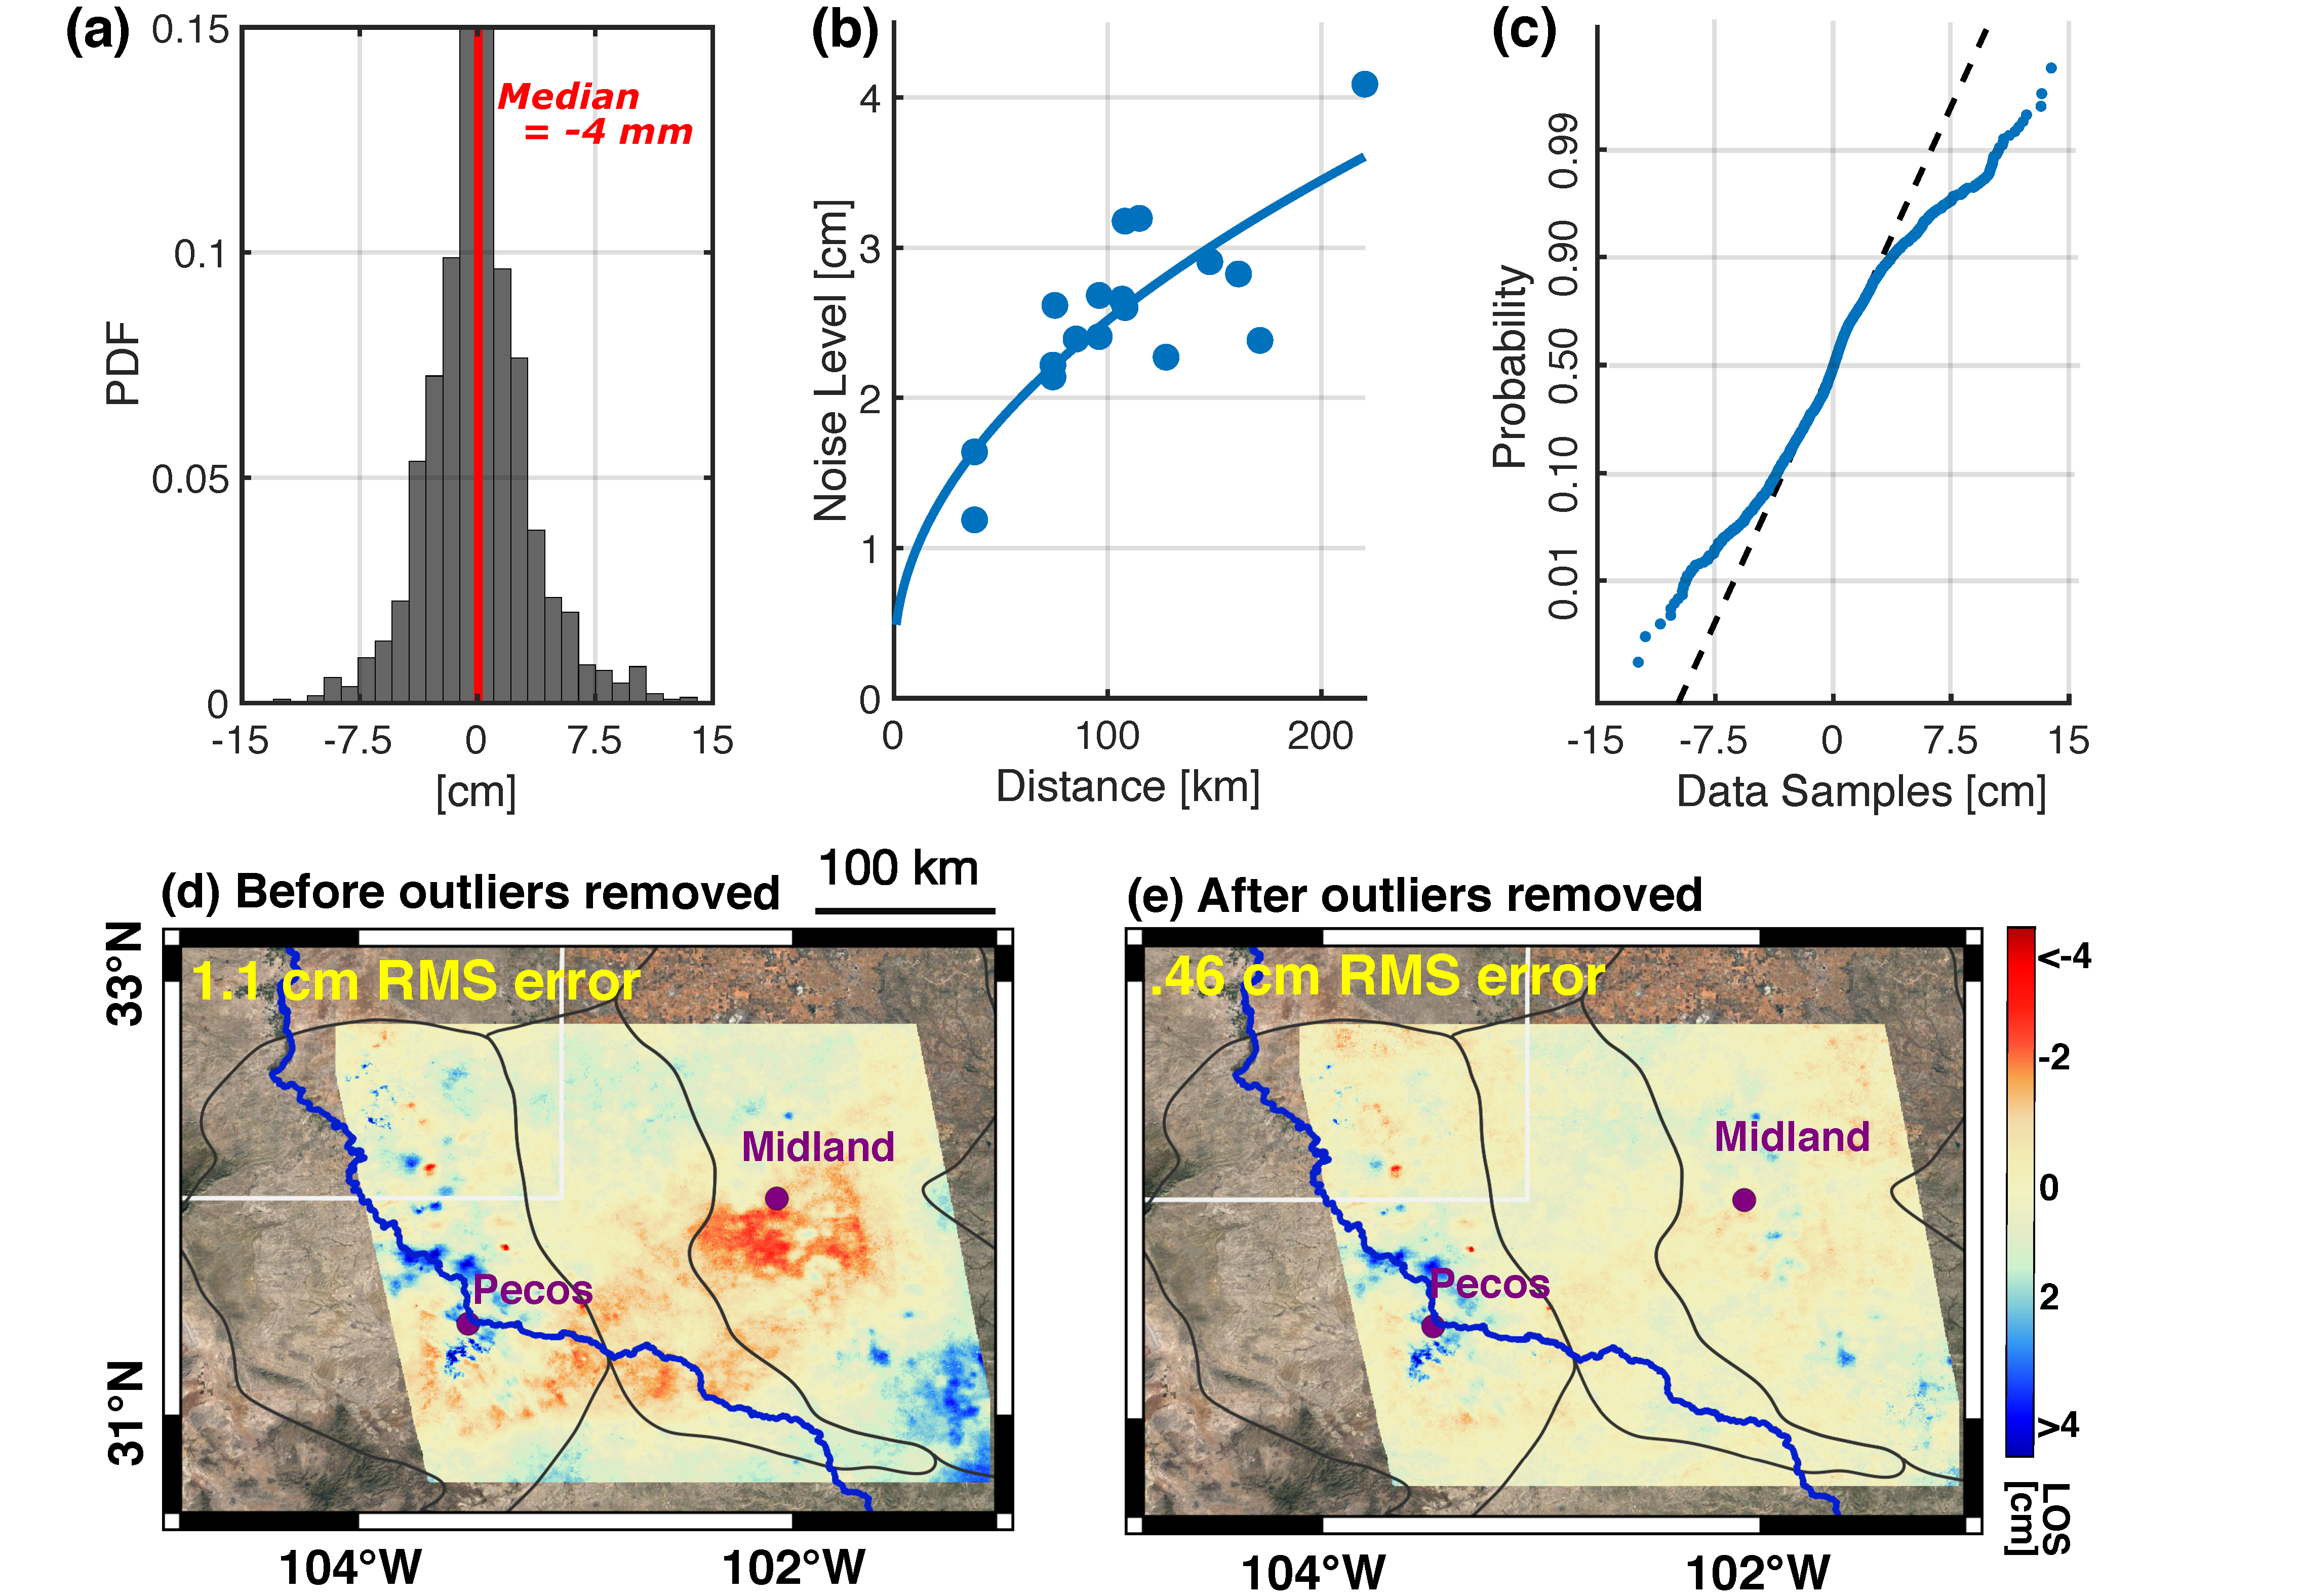
\includegraphics[width=0.95\linewidth]{figures/chapter4-grl/figure2-outlier-removal-5panel.pdf}
	\caption[Noise measurement and tropospheric outliers]{
		(a) LOS measurements (in cm) of all ascending interferograms at the GPS station TXMC. The distribution has a near zero median (-4 mm) and a standard deviation of 3.2 cm. Due to the absence of substantial deformation signals, the standard deviation of the distribution is a measure of LOS turbulent tropospheric noise. (b) The standard deviation of random tropospheric turbulent noise at 13 control locations (blue dots), which increases as the square root of the distance from the InSAR reference point (blue line). (c) A comparison between the tropospheric noise distribution at TXMC with a normal distribution. Dashed line connects the 1st and 3rd quartiles of the data. Troposphere noise following a normal distribution would match the dashed line, and non-Gaussian tails are present. 
	}
	\label{fig:ch4-outliers}
\end{figure}



%When severe tropospheric noise (e.g. storms or heat waves) affects interferograms, the resulting measurement distribution at a given pixel can contain large non-Gaussian tails. 
%Identifying and removing InSAR measurement outliers is crucial for achieving millimeter level accuracy. 
Because severe tropospheric noise may only impact a portion of a SAR image, we identified InSAR measurement outliers at each pixel independently as follows. Given $N$ SAR acquisitions, there are up to $N-1$ InSAR LOS measurements at a pixel of interest that contain the common tropospheric noise of the $k^{th}$ SAR scene. We defined $u_{k,n}$ as the $n^{th}$ such LOS measurement, and $\bar{u}_k$ as the mean absolute measurement:
\begin{equation}
	\bar{u}_k  = \frac{1}{N-1} \sum_{n=1}^{N-1} |u_{k,n}|  
\end{equation}
We labeled $u_{k,n}$ (for all $n$) as outlier measurements if $\bar{u}_k > \mathrm{median}(\mathbf{\bar{u}}) + 4 \sigma_{\mathrm{MAD}}$, where $\mathbf{\bar{u}}=[\bar{u}_1,...,\bar{u}_N]$, and $\sigma_{\mathrm{MAD}}=1.483 \cdot \mathrm{MAD}(\mathbf{\bar{u}})$. Here we employed a robust statistics measure, the median absolute deviation (MAD), for estimating the spread of data samples in the presence of outliers \citep{Hampel1974InfluenceCurveIts, Rousseeuw2011RobustStatisticsOutlier}. Given a vector $\mathbf{x}$ that contains $M$ data samples, $\mathrm{MAD}(\mathbf{x})$ is defined as:
\begin{equation}
	\mathrm{MAD}(\mathbf{x}) =  \underset{m = 1,\ldots M}{\mathrm{median}} \left( \bigr\lvert  x_m - \mathrm{median}(\mathbf{x})  \bigr\rvert \right)
\end{equation}
where $x_m$ is the $m^{th}$ data sample. 



%To account for the large variation in look angle within one Sentinel-1 Interferometric Wide (IW) swath image, we used the LOS unit vector at each pixel location Figure \ref{fig:los-map})) in the LOS decomposition.





%In this study, used the Sentinel-1 interferograms from path 78 and path 85 processed as described in Section \ref{sec:ch2-insar-processing}.
%We solved for the average LOS velocities over three periods of interest: Nov. 2014 to Jan. 2017, Nov. 2014 to Jan. 2018, and Nov. 2014 to Jan. 2019. Over each time period $T_j$, we computed the cumulative LOS surface deformation as the product of $v_{avg,j}$ and $T_j$. We also solved for the vertical and eastward deformation in the region where path 78 and 85 overlap (see Section \ref{sec:ch2-insar-decomp}) using the LOS unit vector at each pixel location Figure \ref{fig:los-map})) in the LOS decomposition.

\section{Line-of-sight Decomposition}
\label{sec:ch2-insar-decomp}


\begin{figure}
	\centering
	%	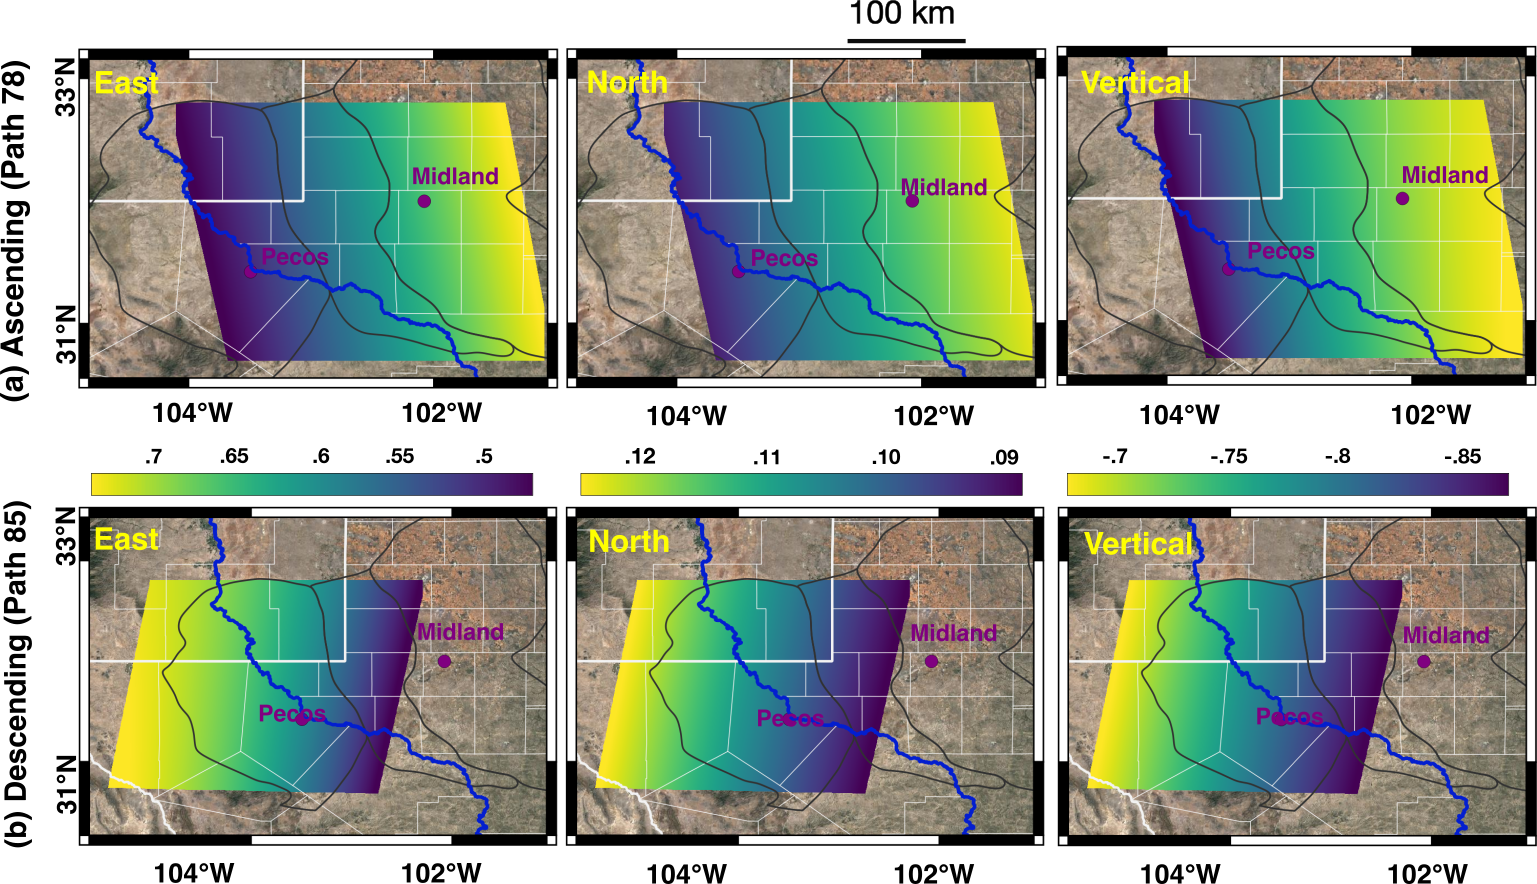
\includegraphics[width=.98\textwidth]{paper1-permian/figures/supplement/figureS2-los.pdf}
	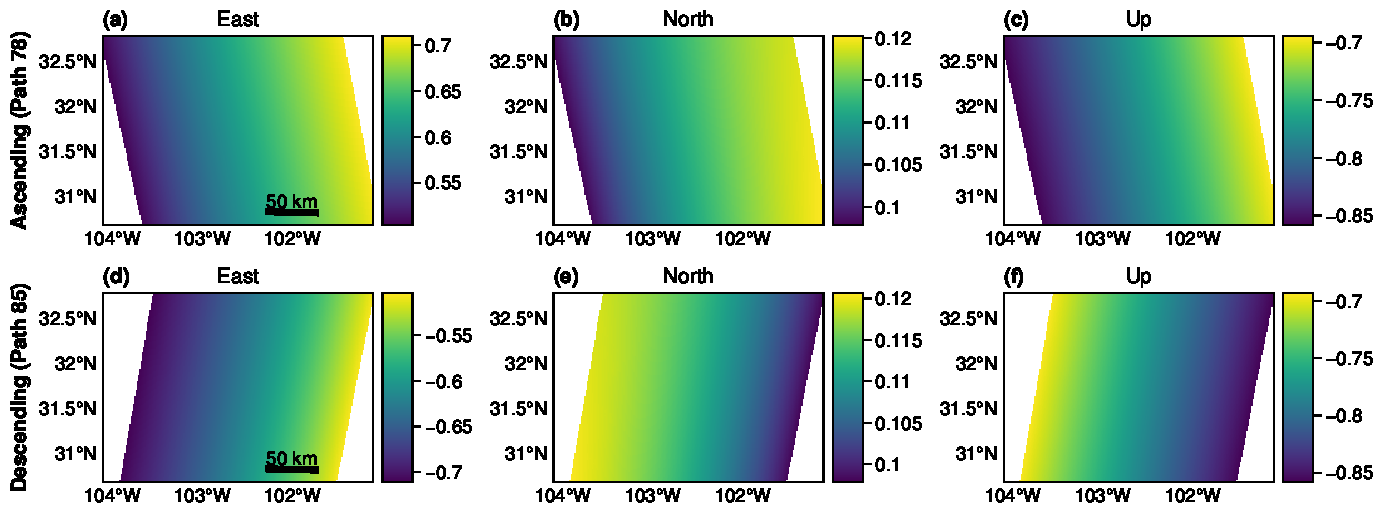
\includegraphics[width=.98\textwidth]{figures/chapter2-sar/figure_los_enu_coeffs.pdf}
	\caption[East, north, and vertical coefficients of Sentinel-1 LOS vectors]{East, north, and vertical coefficient of the LOS unit vector of all Sentinel-1 path 78 and path 85 pixels. Positive LOS direction points away from the satellite to the ground.
	}
	\label{fig:los-map}
\end{figure}

An interferogram measures surface deformation between the two SAR acquisition times along the radar line-of-sight (LOS) direction. The LOS deformation, $u_{LOS}$, can be written as: 
\begin{align}
	u_{LOS}= \alpha_{e} u_{e} + \alpha_{n} u_{n} + \alpha_{u} u_{u}
\end{align}
where $u_{e}$, $u_{n}$ and $u_{u}$ are the east, north and up displacements, respectively. The radar look vector $\alpha = [\alpha_e, \alpha_n, \alpha_u]$ can be calculated from the known imaging geometry at every pixel location. This varies significantly for Sentinel-1 due to the $ \sim$250 km wide swath (Figure \ref{fig:los-map}). 


In regions where InSAR data are available from two LOS directions, we can decompose the ground motion into its eastward and vertical components.
To perform the decomposition, we first write $u_{asc}$ and $u_{desc}$ in terms of $u_e$, $u_n$ and $u_u$:
\begin{align}
	u_{asc} &= \alpha_{a,e} u_{e} + \alpha_{a,n} u_{n} + \alpha_{a,u} u_{u}\\
	u_{desc} &= \alpha_{d,e} u_{e} + \alpha_{d,n} u_{n} + \alpha_{d,u} u_{u}
\end{align}
We can express $u_e$ and $u_u$ as:
\begin{align}
	u_{e} &\approx  \frac{1}{\beta}  \left[\alpha_{d,u}  u_{asc} - \alpha_{a,u} u_{desc} \right] \\
	u_{u} &\approx  \frac{1}{\beta}  \left[\alpha_{a,e} u_{desc} - \alpha_{d,e}  u_{asc}  \right] 
\end{align}
where  $ \beta = {\alpha_{a,e} \alpha_{d,u}- \alpha_{d,e} \alpha_{a,u}} $.
Because Sentinel-1 satellites are operating in a near-polar orbit, the north look coefficients $\alpha_{a,n}$ and $\alpha_{d,n}$ are both relatively small. Ignoring 1 cm northward motion in $u_n$ only leads to $\sim$ 0.1-0.2 mm error in $u_e$ and $\sim$ 1 mm error in $u_u$ at most locations.  





%\subsection{Uncertainty Propagation through LOS decomposition}
%\label{sec:ch2-decomp-uq-prop}
%Since the LOS decomposition is a linear operation, given two LOS uncertainties, we can use linear uncertainty propagation theory to determine the vertical/horizontal uncertainties.
%
%TODO: move this to appendix or not?




\section{Time series comparisons and outlier removal}
\label{sec:ch4-ts-compare-result}

%- Describe the GPS comparisons for the stacking+outlier results, cutting errors by 2x [Maybe with your uncertainty tables]
%- Bottom half of outlier figure showing the visible artifacts removed
%- Talk about the time series comparison figure, how each had problems, then after outlier removal most converge (+ table quantifying the before/after)
%- conclude all methods converge and we use a simple stacking with outlier removal to calculate cumulative deformation.
%



Using the 13 GPS east, north, and up time series as ground truth, we quantified the errors in the InSAR stacking solutions before and after the outlier removal. 
%There are 13 permanent GPS stations in the ascending SAR footprint.
At each GPS location, we projected the GPS time series to the radar line-of-sight (LOS), and we computed the GPS-inferred average LOS velocity through a linear regression. Table \ref{tab:gps-error-78} shows the root mean square (RMS) and the worst-case absolute differences between InSAR and GPS inferred average LOS velocities over the three study periods. Similarly, there are 5 permanent GPS stations in the descending SAR footprint, and Table \ref{tab:gps-error-85} shows the uncertainty in the descending stacking solutions using these 5 GPS stations as control. Both Table \ref{tab:gps-error-78} and Table \ref{tab:gps-error-85} show that our outlier removal algorithm reduced the uncertainty in InSAR stacking solutions by a factor of $\sim$2, down to 1-3 mm/year across the basin. For a given period of interest $T_j$, the LOS velocity error $ E_{vel,j} $ propagates into the cumulative deformation error $ E_{c, j} $ as $ E_{c,j} = E_{vel,j} \cdot T_j $. 


\begin{table}
	\caption{InSAR ascending LOS velocity estimation errors (in mm/year) using the stacking method}
	\centering
	\begin{tabular}{|c|c|c|}
		\hline 
		& Before the outlier removal & After the outlier removal \\
		& (RMS / Worst) & (RMS / Worst) \\
		\hline
		Nov. 2014 - Jan. 2017 & 3.8 / 9.5         & 1.9 / 5.9       \\\hline
		Nov. 2014 - Jan. 2018 & 3.3 / 7.1         & 1.3 / 2.5       \\\hline
		Nov. 2014 - Jan. 2019 & 2.0 / 6.1         & 1.1 / 2.5       \\\hline                
	\end{tabular}
	\label{tab:gps-error-78}
\end{table}

\begin{table}
	\caption{InSAR descending LOS velocity estimation errors (in mm/year) using the stacking method}
	\begin{tabular}{|c|c|c|}
		\hline 
		& Before the outlier removal & After the outlier removal \\
		& (RMS / Worst) & (RMS / Worst) \\
		\hline 
		Nov. 2014 - Jan. 2017 & 7.8 / 13.8                            & 2.9 / 5.0                          \\\hline
		Nov. 2014 - Jan. 2018 & 3.7 / 7.5                             & 2.7 / 5.6                          \\\hline
		Nov. 2014 - Jan. 2019 & 1.6 / 2.8                             & 0.8 / 1.6  \\\hline     
	\end{tabular}
	\label{tab:gps-error-85}
\end{table}




\begin{figure}
	\centering
	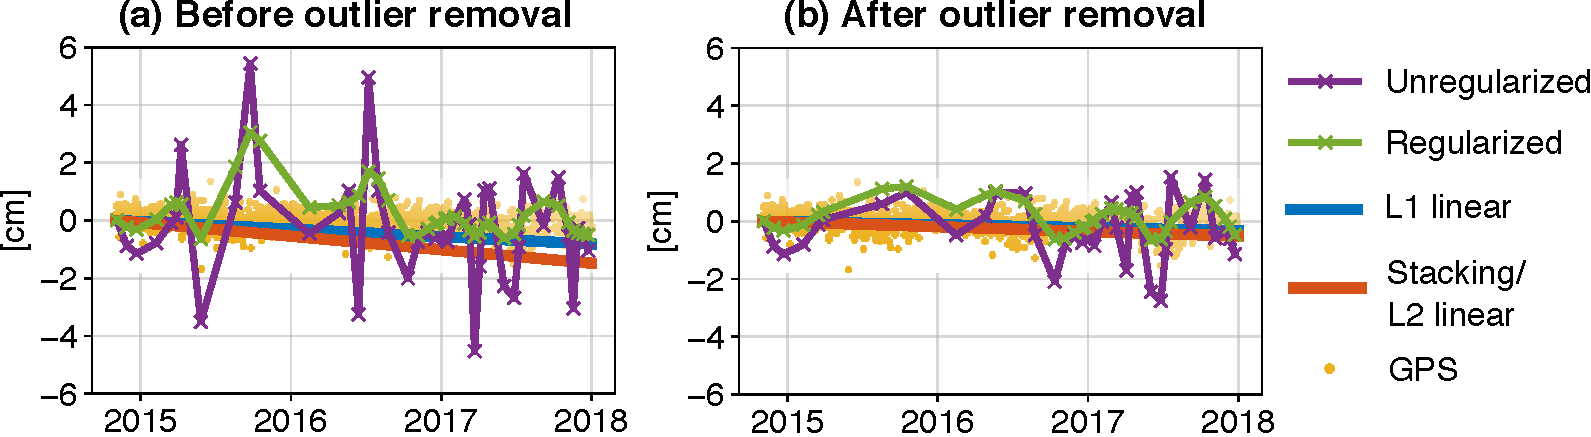
\includegraphics[width=\textwidth]{figures/chapter4-grl/supplement/figureS5-compare-insar-2panel.pdf}
	\caption[Comparisons of InSAR SBAS solutions]{Comparisons of InSAR unregularized SBAS time series (purple), regularized SBAS time series (green), linear deformation trend estimated by minimizing the $L_1$-norm of the residuals (blue), and the $L_2$-norm of the residuals/ stacking approach (red)  (a) before and (b) after removing LOS measurement outliers. ENU GPS data from station TXSO has been projected onto the radar LOS (orange dots).}
	\label{fig:ch4-compare-ts}
\end{figure}


\begin{table}
	\caption{Errors (in mm) in four SBAS ascending LOS deformation (Nov. 2014 - Jan. 2018) solutions}
	\centering
	\begin{tabular}{|c|c|c|}
		\hline 
		& Before the outlier removal & After the outlier removal \\
		& (RMS / Worst) & (RMS / Worst) \\
		\hline
		Unregularized &  22 / 99     &  14 / 43         \\\hline
		Regularized   &    14 / 63   &   10  / 27       \\\hline
		L1 linear deformation          &   7 / 11      & 4 / 8      \\\hline
		L2 linear deformation          &   10 / 22        & 4 / 8      \\\hline
	\end{tabular}
	\label{tab:compare-errors}
\end{table}





%To evaluate the performance of our InSAR processing strategy, 
We projected GPS data recorded at 13 control stations onto the LOS directions to use as ground truth. The differences between InSAR and GPS inferred average LOS velocities were used as a measure of the uncertainty in the InSAR surface deformation solutions. 
We found that stacking reduces the impact of random Gaussian turbulent noise by $ \sim \sqrt{N} $, where $ N $ is the number of SAR acquisitions. The outlier removal algorithm further reduces the uncertainty in the LOS velocity estimates by a factor of 2, down to 1-3 mm/year across the basin. For example, the average InSAR velocity along the ascending LOS direction between Nov. 2014 and Jan. 2018 shows a root mean square (RMS) error of 3.4 mm/year before the outlier removal, and 1.5 mm/year after the outlier removal. The presence of InSAR measurement outliers resulted in long-wavelength artifacts ($ \sim $100km and greater) in the cumulative deformation solutions (e.g. Figure \ref{fig:ch4-outliers} (d)), which were automatically mitigated through the pixel-based outlier removal algorithm (e.g. Figure \ref{fig:ch4-outliers} (e)). Additionally, we compared InSAR LOS deformation solutions as derived from (1) the stacking method, (2) a SBAS linear deformation model with $L_1$ and $L_2$-norm penalty functions, and (3) unregularized and regularized SBAS deformation time series (Section \ref{sec:ch4-method-compare}). These InSAR time series algorithms can be implemented using software packages such as Generic InSAR Analysis Toolbox (GIAnT) \citep{Agram2013NewRadarInterferometric}, STAMPS \citep{Hooper2012RecentAdvancesSar}, and LiCSBAS \citep{Morishita2020LicsbasOpenSource}. Removing the detected outliers leads to more accurate and consistent surface deformation solutions in all three cases. 



%Little surface deformation occurred between Nov. 2014 and Jan. 2019 at the 13 GPS permanent GPS stations. 
At each GPS location, we projected the GPS time series to the radar line-of-sight (LOS), and we used the GPS-inferred average LOS velocity (0-3 mm/year) as ground truth. Table \ref{tab:compare-errors} shows the root mean square (RMS) and the worst-case absolute differences between InSAR and GPS inferred average LOS velocities between Nov. 2014 and Jan. 2018 as derived from the four InSAR time series methods. We found that InSAR tropospheric noise has a strong influence on all the surface deformation solutions before removing the measurement outliers. As an example, Figure \ref{fig:ch4-compare-ts} (a) shows the ascending LOS solutions between Nov. 2014 and Jan. 2018 at the GPS station TXSO before removing InSAR measurement outliers. The random tropospheric noise creates up to $\sim$6 cm of error in the unregularized SBAS surface deformation time series. This error can be reduced by increasing $ \alpha$ in Equation \eqref{eq:ch4-sbas}. As $\alpha$ increases, the LOS deformation time series converge to the $L_2$ linear deformation (constant velocity) solution. However, there are visible cm-level tropospheric artifacts in the cumulative deformation solutions by using either $L_1$ or $L_2$ linear deformation models (e.g. Figure \ref{fig:ch4-outliers}(d)).   



After removing InSAR outlier measurements associated with extreme local weather events (Section \ref{sec:ch4-method-compare}), all SBAS time series methods produce more accurate and consistent deformation trends (Figure \ref{fig:ch4-compare-ts} (b)). The unregularized SBAS time series still contain up to $\sim$3 cm of tropospheric noise, which leads to long-wavelength artifacts in the basin-wide deformation maps. The $ L_1 $ and $ L_2 $ linear deformation solutions show close agreement ($<$ 2 mm difference) at all GPS stations. Since both methods suggest a deformation trend consistent with the stacking approach, we chose the simple stacking method as the final processing strategy for estimating cumulative surface deformation in the Permian Basin.



\begin{figure}
	\centering
	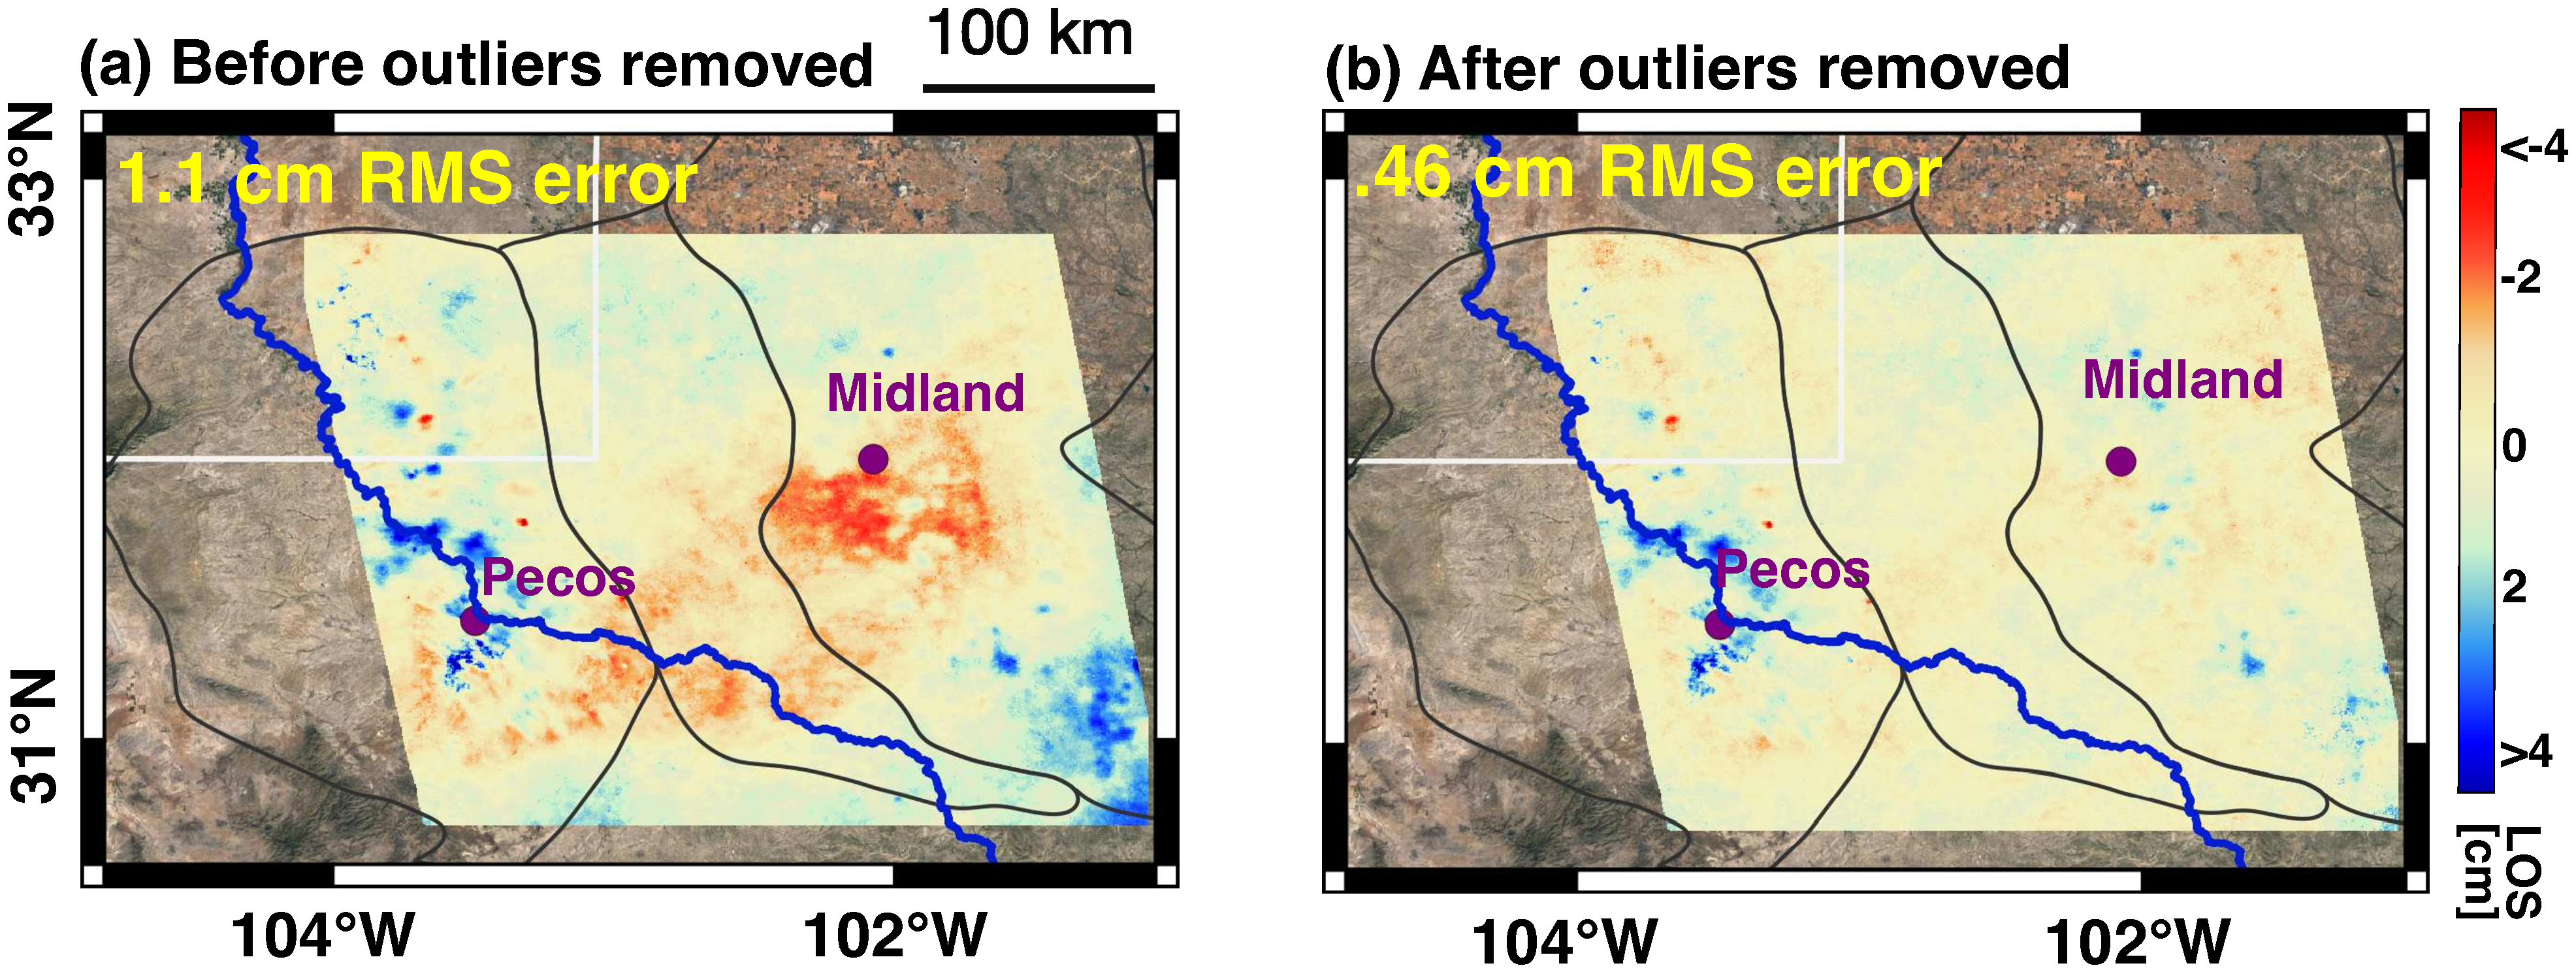
\includegraphics[width=0.99\linewidth]{figures/chapter4-grl/outlier-bottom-only.pdf}
	\caption[Tropospheric outlier removal comparison]{
		Cumulative ascending LOS deformation solutions (Nov. 2014 - Dec. 2017) 
		(a) before and (b) after excluding InSAR outlier measurements. Note that 1.1 cm cumulative error over 3 years is equivalent to 3.5 mm/year RMS error in the velocity estimate.}
	\label{fig:ch4-outliers-visual}
\end{figure}


%
%\subsection{InSAR LOS velocity estimation error}
%\label{sec:error-quant}


\section{Surface deformation in the Permian Basin}



The Sentinel-1 cumulative LOS deformation solutions reveal numerous surface deformation features over the oil-producing region in the Permian Basin (Figure \ref{fig:ch4-insar-los}). From the ascending geometry, we observed no substantial deformation in the Central Basin Platform, where oil and gas are mostly produced from conventional reservoirs. In the Midland and Delaware Basins, we observed an accelerating surface deformation rate between Nov. 2014 and Jan. 2019, which coincides with the sharp rise of oil production from unconventional reservoirs in 2017 and 2018. For example, a 30 km$^2 $ area northwest of Pecos shows approximately 0.5 cm cumulative LOS deformation between Nov. 2014 and Jan. 2017, 1.5 cm between Nov. 2014 and Jan. 2018, and over 5.5 cm from Nov. 2014 to Jan. 2019. The greatest number of observable signals are present in 2018 when peak production occurred in the region. Similarly, from the descending geometry, we find no substantial deformation in the Central Basin Platform and an increasing rate of surface deformation in the Delaware Basin. 


\begin{figure}
	\centering
	%	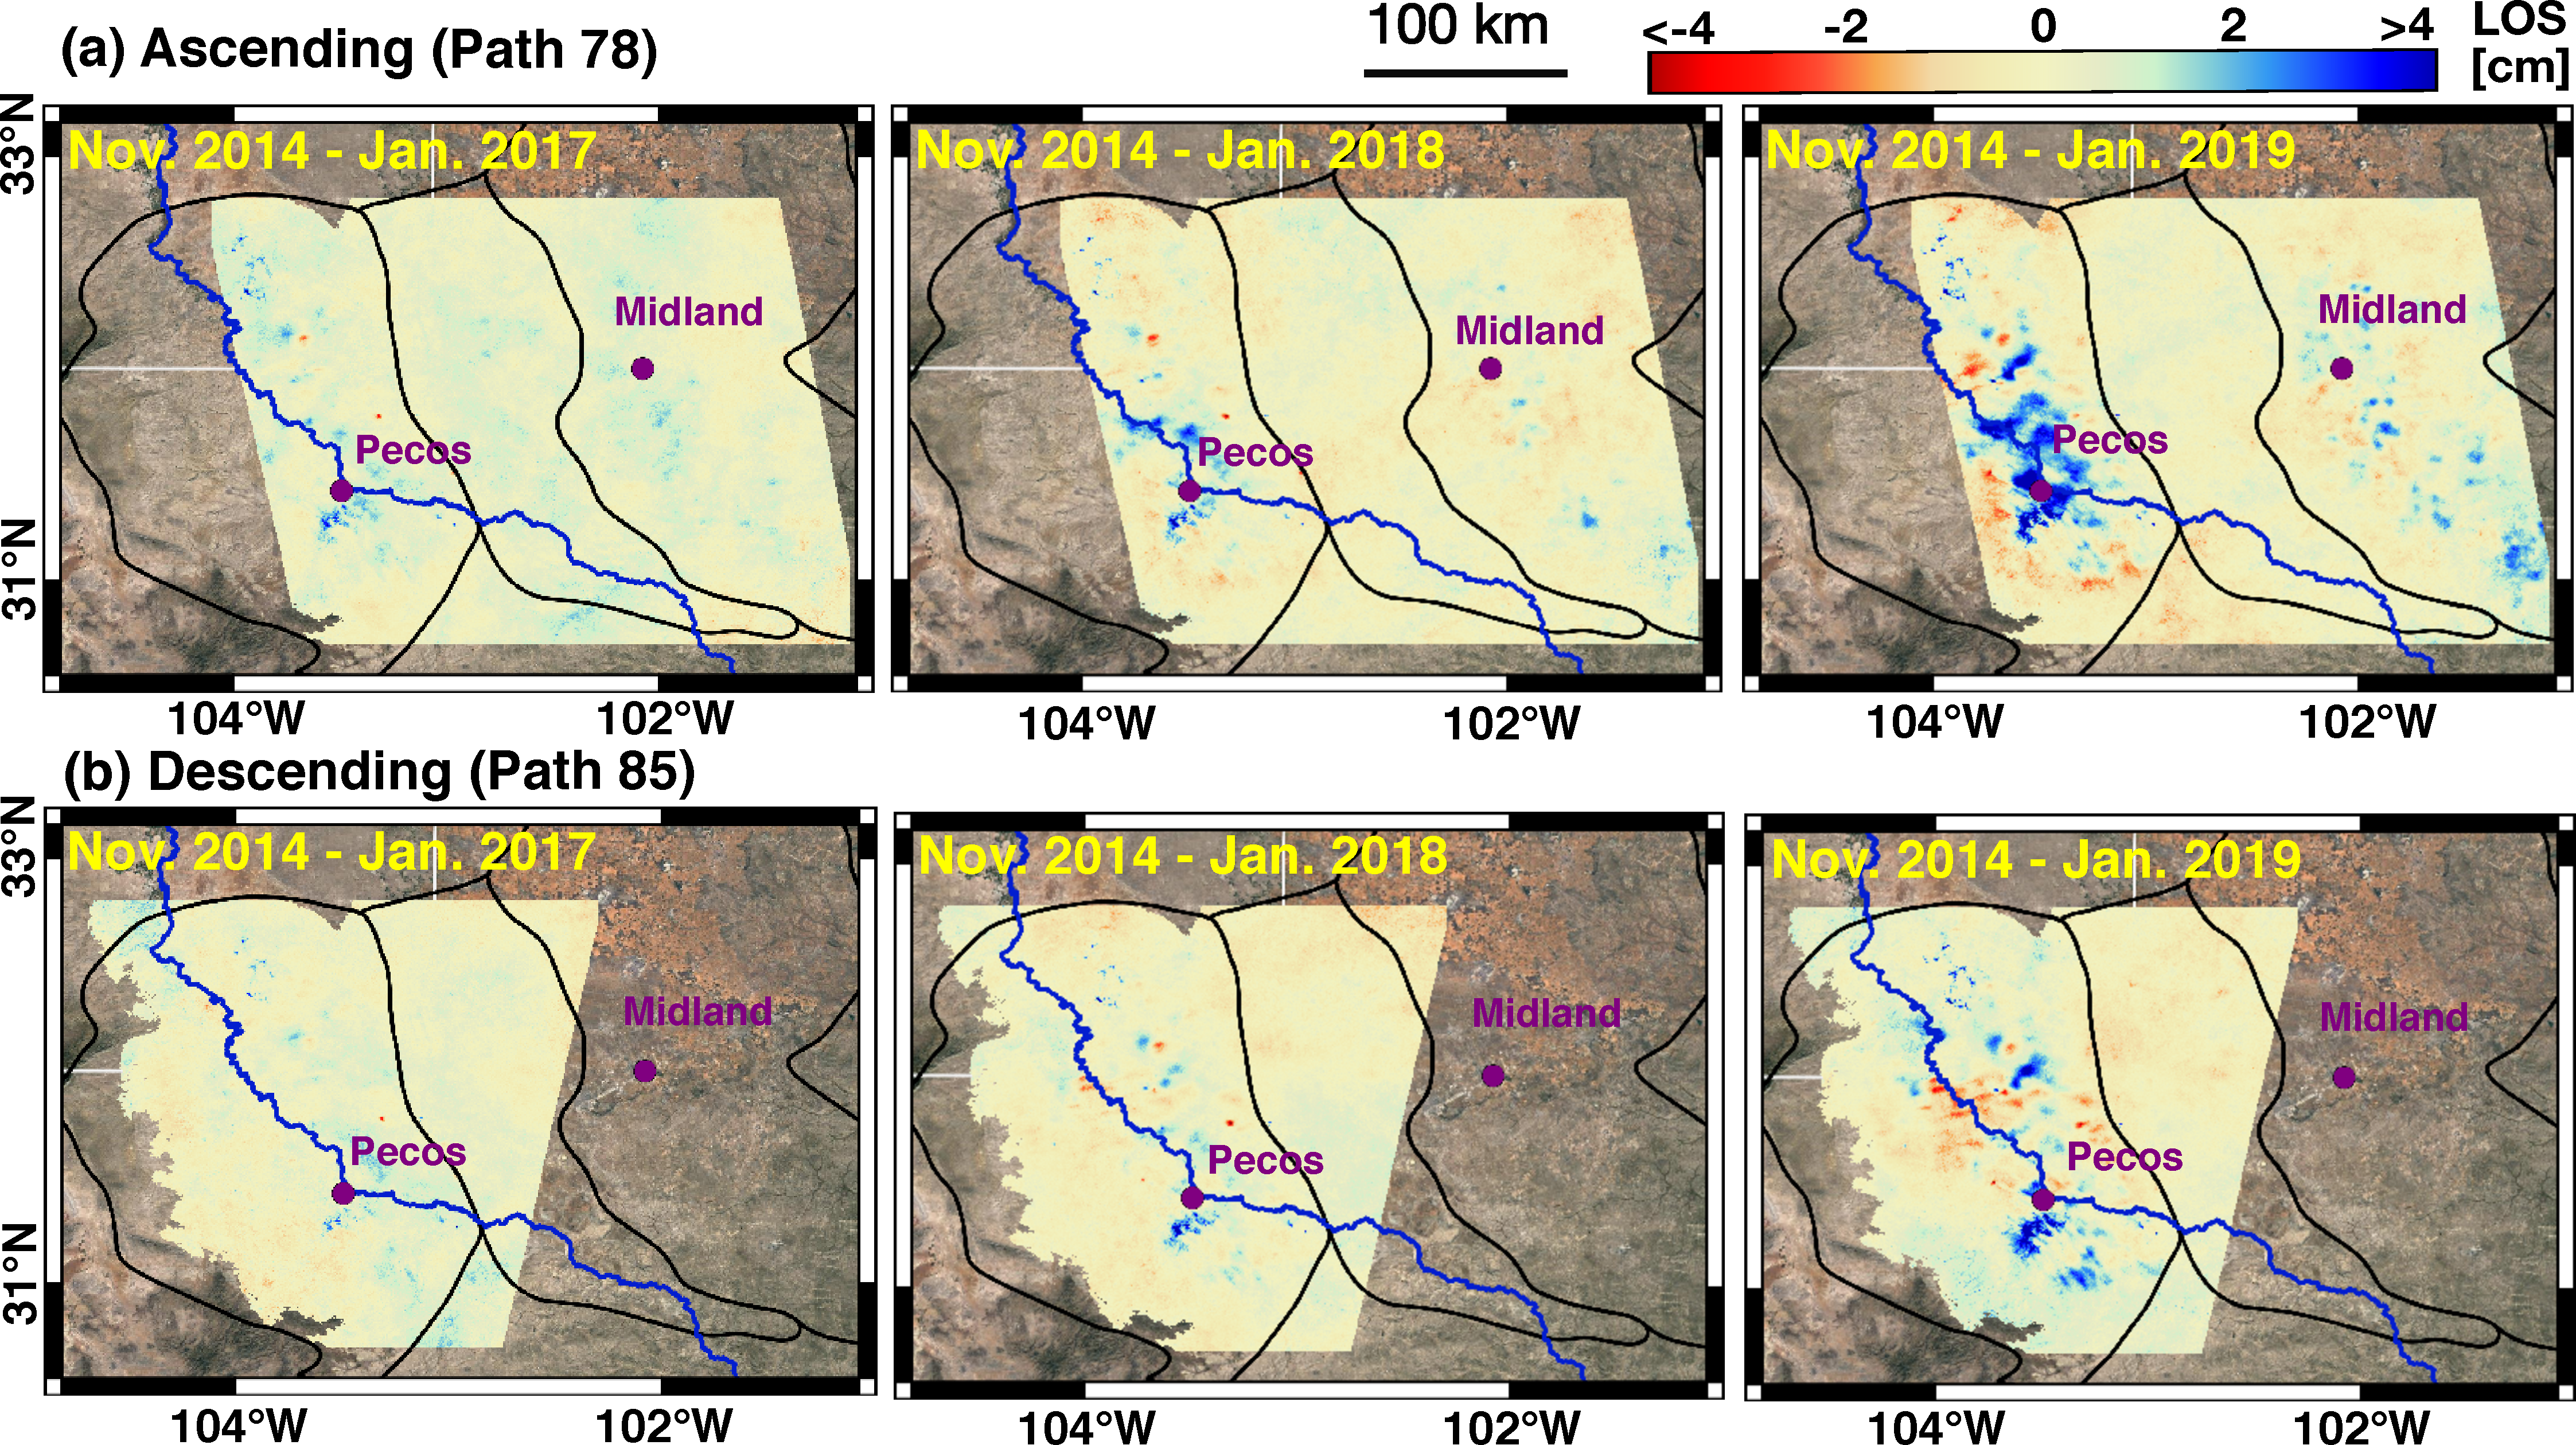
\includegraphics[width=.99\linewidth]{figures/chapter4-grl/figure3-los-insar.pdf}
	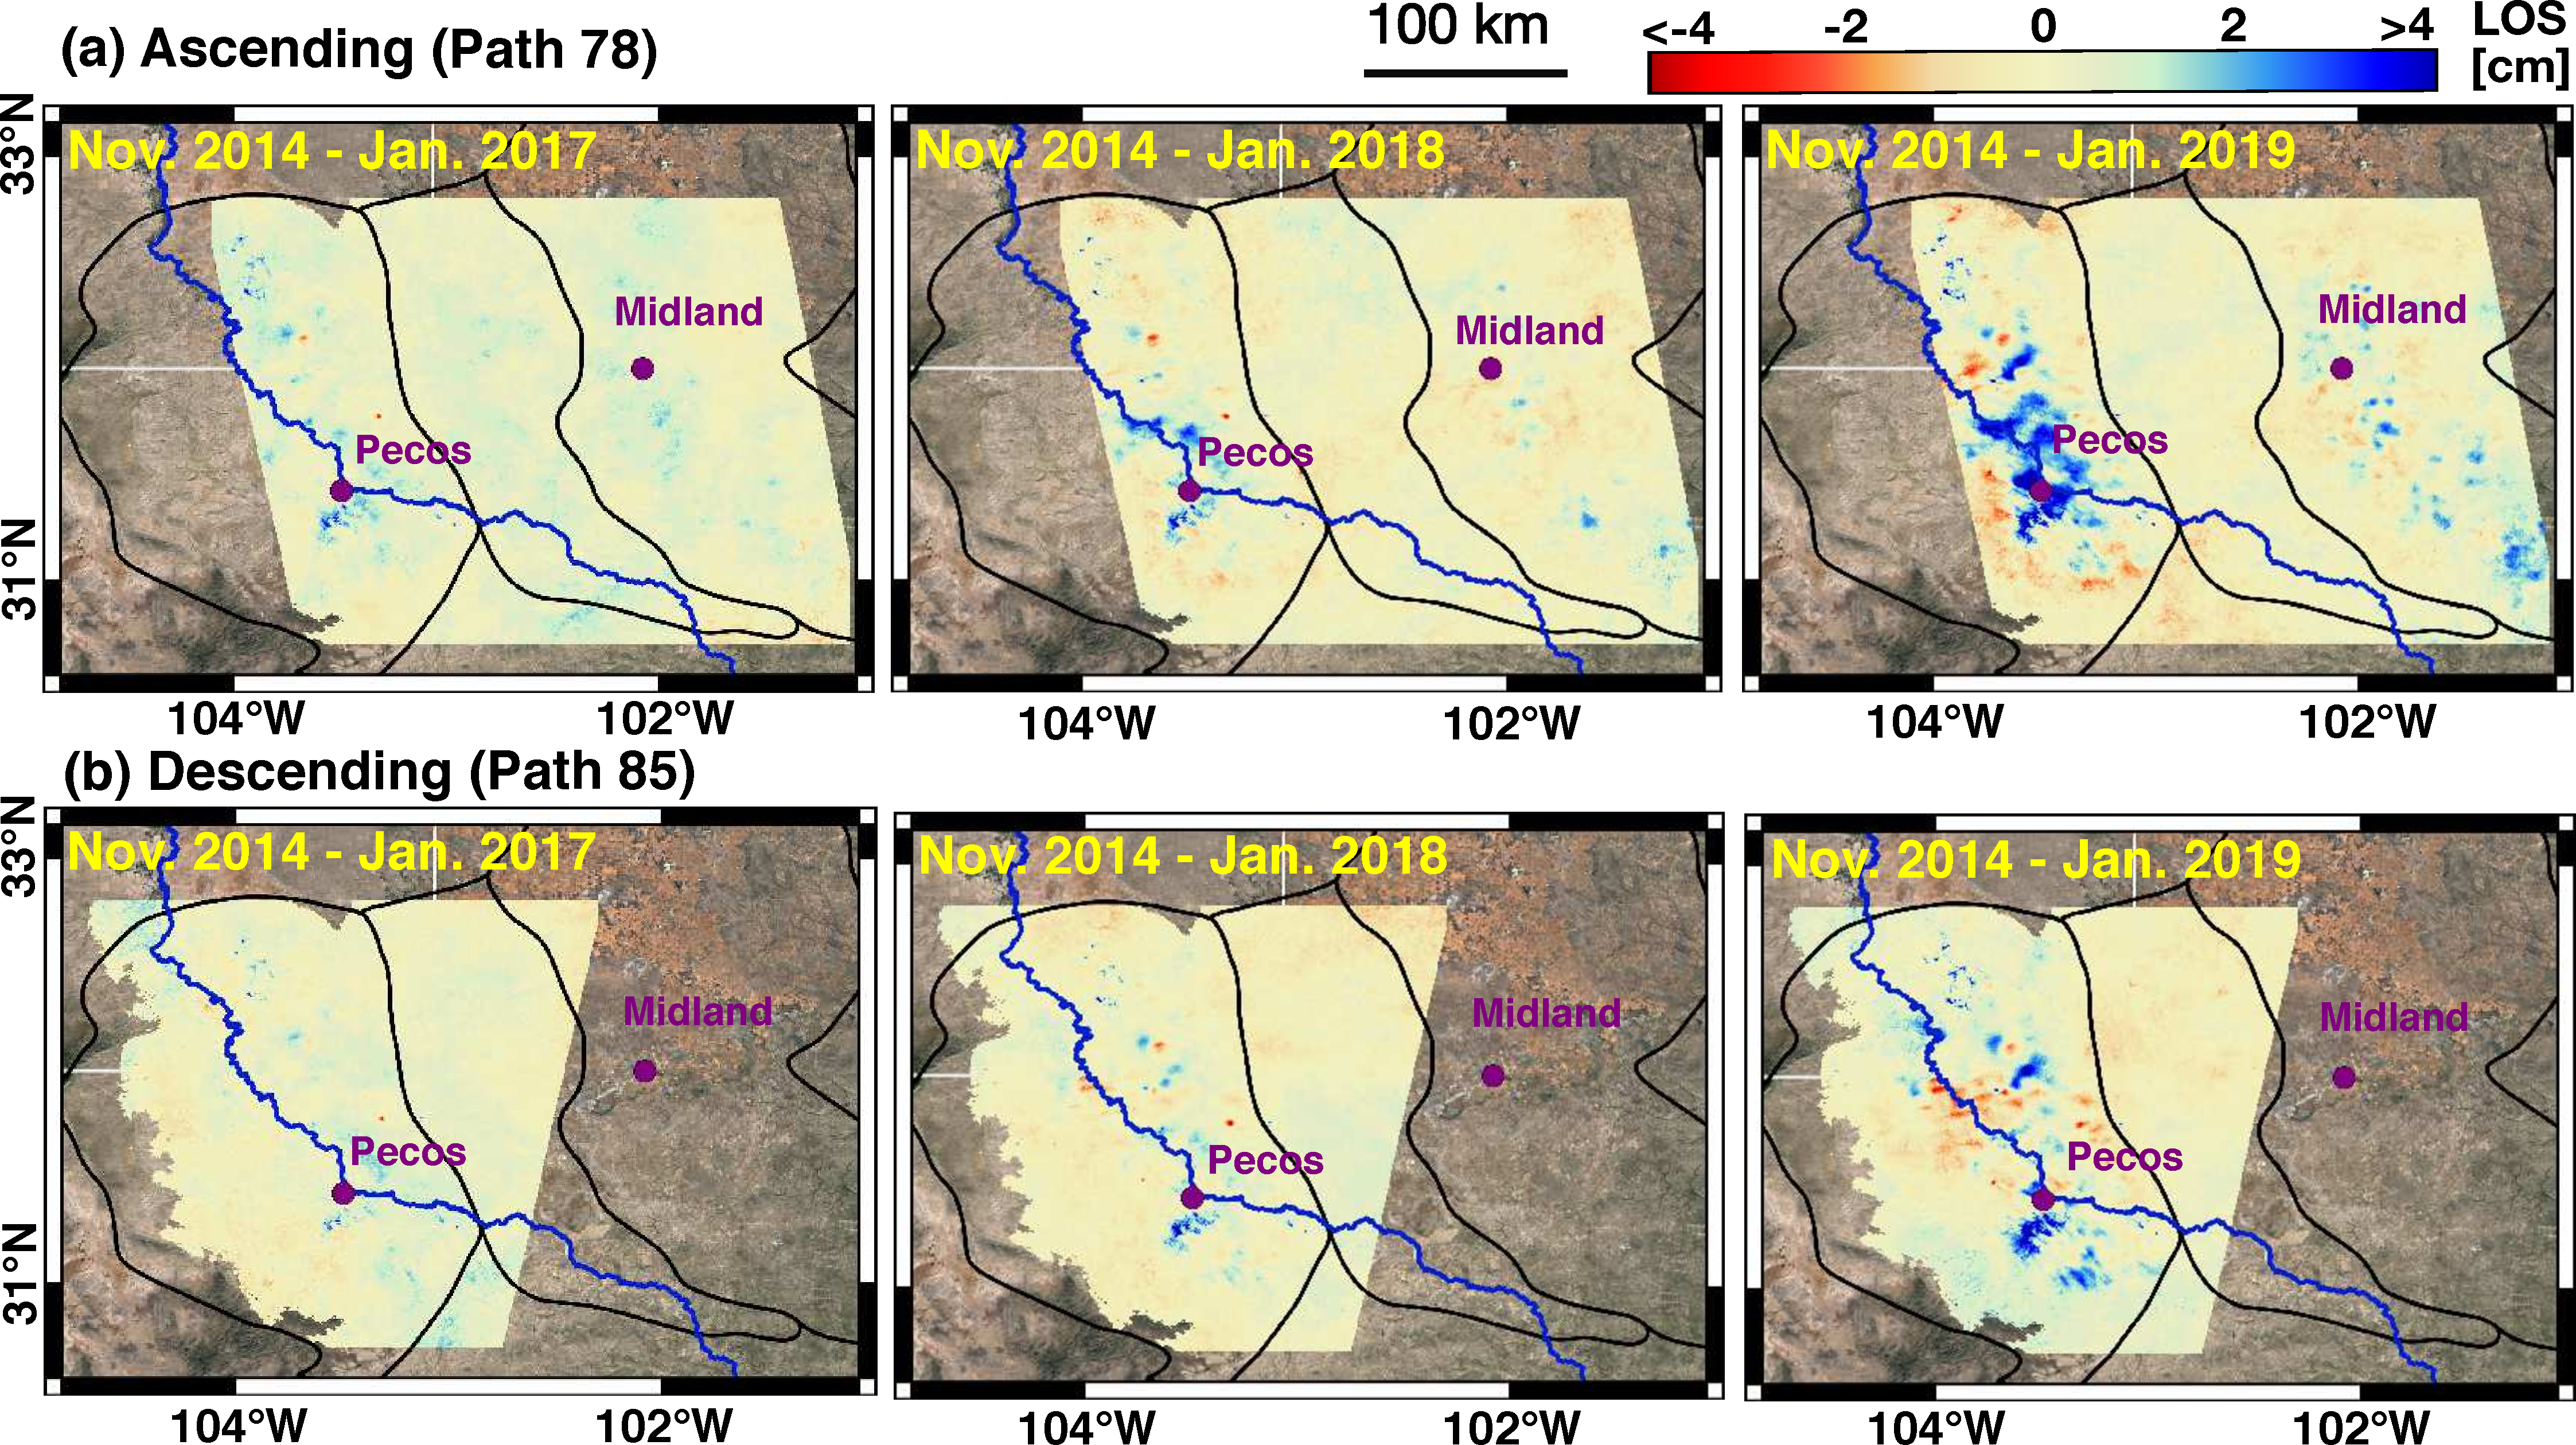
\includegraphics[width=.99\linewidth]{figures/chapter4-grl/figure3-los-insar-small.pdf}
	\caption[Cumulative LOS deformation for path 78 and path 85]{Cumulative LOS deformation (Nov. 2014 - Jan.2017; Nov. 2014 - Jan.2018; Nov. 2014 - Jan. 2019) as inferred from Sentinel-1 (a) ascending path 78, and (b) descending path 85 data over an 80,000 square km oil-producing region of the Permian Basin. Here a subsidence or eastward deformation signal leads to a positive LOS measurement in the ascending geometry, and a subsidence or westward deformation signal leads to a positive LOS measurement in the descending geometry. Areas with $>$1200 m altitude are masked due to the low oil production activity in mountainous regions.}
	\label{fig:ch4-insar-los}
\end{figure}

\begin{figure}
	\centering
	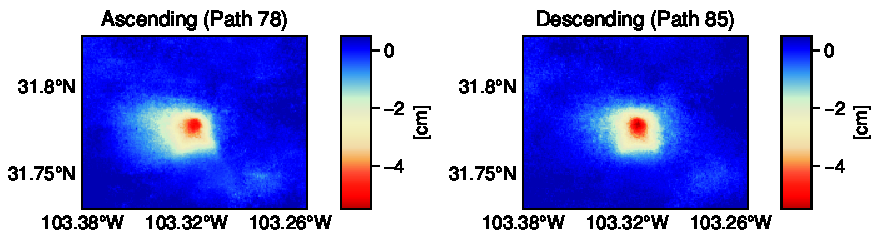
\includegraphics[width=\textwidth]{figures/chapter2-sar/injection-asc-desc.pdf}
	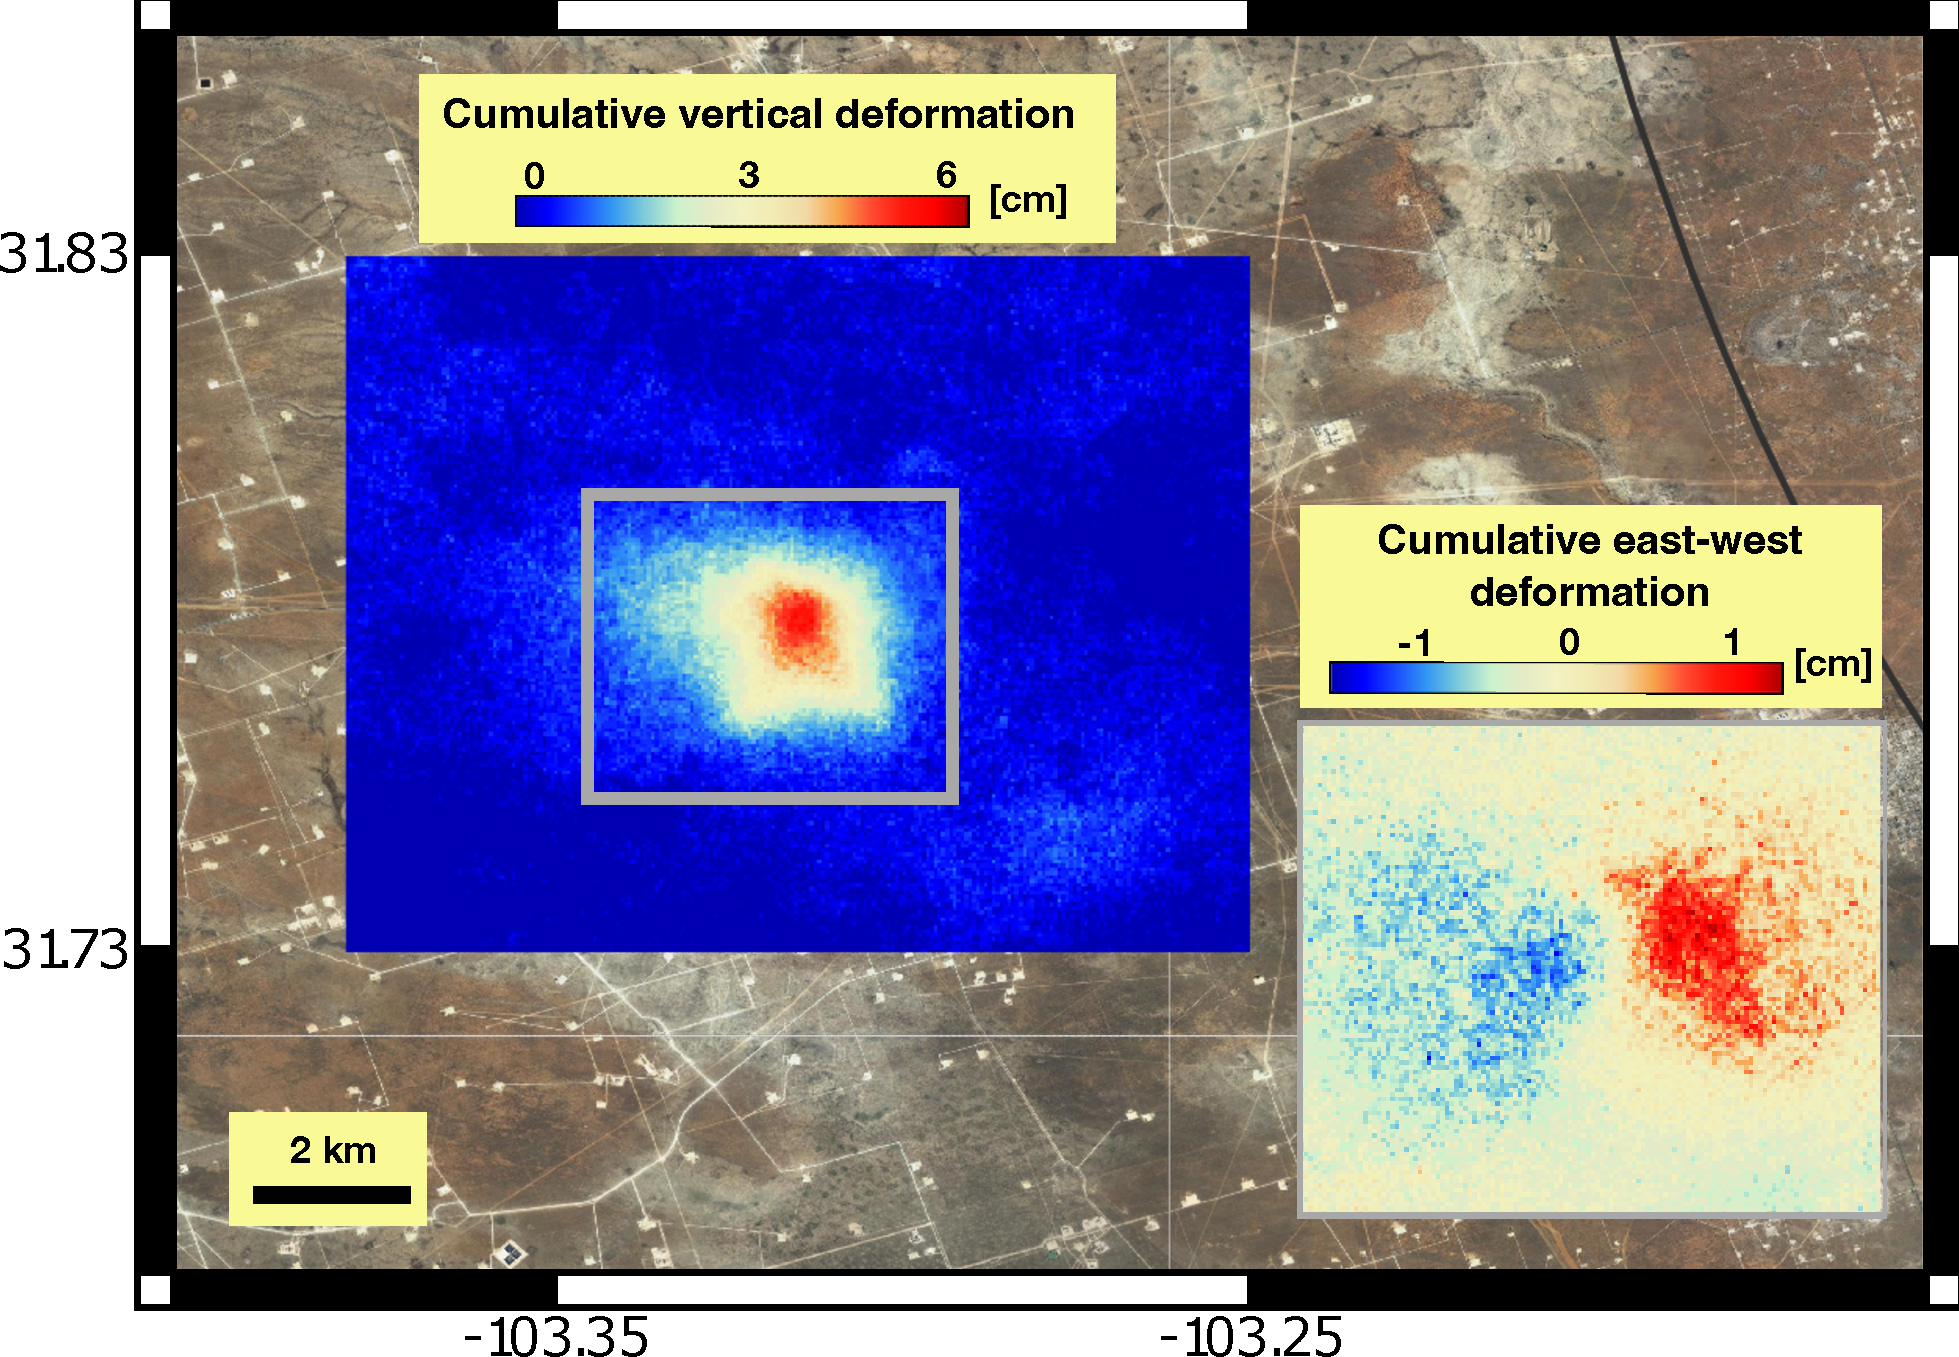
\includegraphics[width=\textwidth]{figures/chapter2-sar/injection-kim-lu}
	%	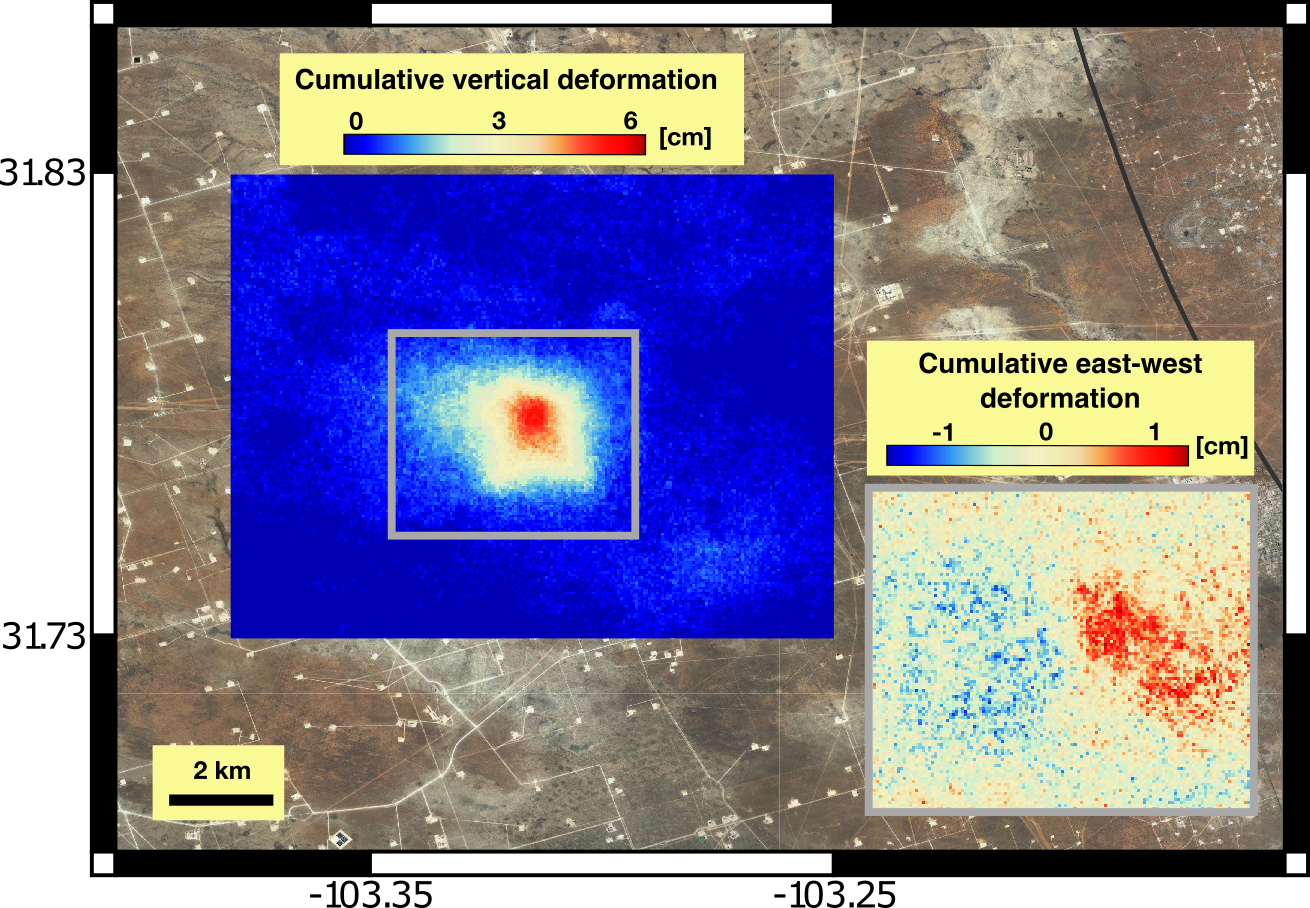
\includegraphics[width=\textwidth]{paper1-permian/figures/supplement/figureS3-injection-kim-lu.pdf}
	\caption[Vertical and horizontal deformation near Winkler County, TX]{
		(top) Ascending and descending line-of-sight cumulative deformation between November 2014 and April 2017. Red indicates motion toward each satellite.
		(bottom) Cumulative vertical and horizontal surface deformation due to wastewater injection in Winkler County, TX. The horizontal motion here is $\sim$ 20\% of the vertical motion, with up to $\sim$ 5.5 cm of uplift and $\sim$ 1.2 cm of east-west motion. This localized deformation feature was originally reported in \cite{Kim2018AssociationLocalizedGeohazards}.}
	\label{fig:ch2-injection-kim-lu}
\end{figure}



We decomposed the ascending and descending LOS solutions from Figure \ref{fig:ch4-insar-decomp} to find the horizontal and vertical deformation.
To illustrate the decomposition, Figure \ref{fig:ch2-injection-kim-lu} shows a 12 km x 12 km region centered on a wastewater injection well found by \cite{Kim2018AssociationLocalizedGeohazards} to have injection-related uplift. We observe similar magnitude deformation toward the satellite in both ascending and descending tracks (Figure \ref{fig:ch2-injection-kim-lu} top). After decomposing the two geometries using the LOS vector at each pixel, we observed $\sim$ 5.5 cm of uplift and $\sim$1.2 cm of east-west motion between November 2014 and April 2017 (Figure \ref{fig:ch2-injection-kim-lu} bottom). 

% ORIGINAL:  \cite{Kim2018AssociationLocalizedGeohazards} detected several localized deformation features within the Delaware Basin related to wastewater injection, CO2 injection, and hydrocarbon production using Sentinel-1 InSAR data.  Our LOS decomposition results are consistent with their study at these locations. For example, in a 12 km x 12 km region centered on a wastewater injection well, we observed $\sim$ 5.5 cm of uplift and $\sim$1.2 cm of east-west motion between November 2014 and April 2017 (Figure \ref{fig:injection-kim-lu}). 

\FloatBarrier


In the northern Delaware Basin, where large volumes of oil production and wastewater disposal occurred, the ascending and descending LOS deformation patterns are similar. This means that the observed deformation in this region is primarily vertical (Figure \ref{fig:ch4-insar-decomp} (b) and (e)). The observed subsidence or uplift features between Nov. 2014 and Jan. 2019 are $\sim$ 1-4 cm. In the southern Delaware Basin, \cite{Deng2020SurfaceDeformationInduced} solved for the cumulative LOS surface deformation between Nov. 2014 and Feb. 2019 ($\sim$ 100 km by 60 km) using the ascending Sentinel-1 data (path 78 frames 99-100). In this study, we found that the observed magnitudes of the ascending and descending LOS deformation are different (Figure \ref{fig:ch4-insar-los}), which suggests that both horizontal and vertical deformation occurred in this region. Previous studies near Mesquite, Nevada have shown that confined aquifer pumping in the presence of faults can produce complex asymmetrical deformation patterns with a non-trivial horizontal component \citep{Burbey2008InfluenceGeologicStructures}. In the Pecos area, the largest subsidence patterns ($\sim$ 13 cm over 4 years) occurred $\sim$ 15 km south of Pecos, and the largest eastward motion ($\sim$ 3-4 cm over 4 years) occurred near the town of Pecos along a line transect (Figure \ref{fig:ch4-insar-decomp} (c) and (f)). The observed linear deformation patterns parallel the inferred favorable fault plane orientation (a strike angle $\sim$ 300 degree lining up with the measured $S_{Hmax}$ direction) proposed by \cite{LundSnee2018StateStressPermian}, and they also align with a cluster of recent shallow earthquakes ($<$ 3 km depth) cataloged by TexNet.



\begin{figure}
	\centering
	%	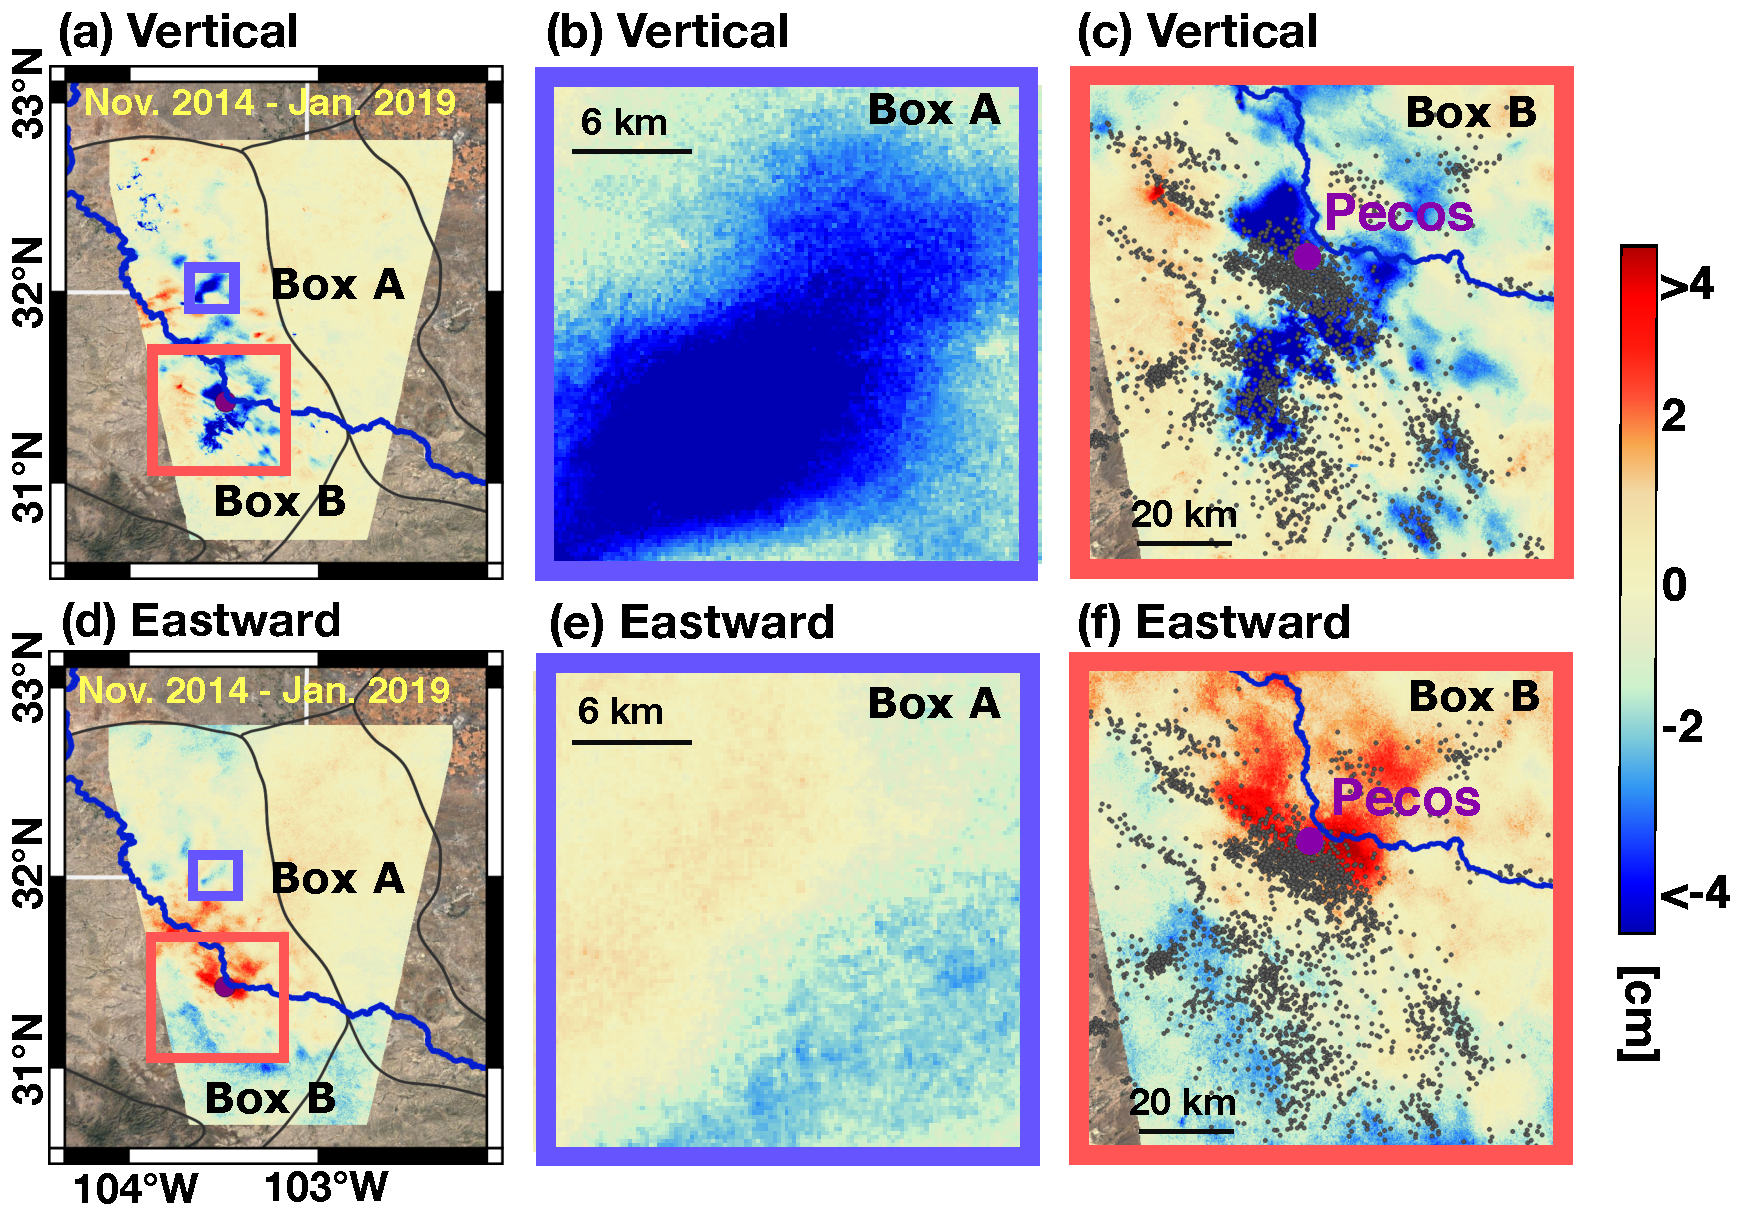
\includegraphics[width=0.96\linewidth]{figures/chapter4-grl/figure4-east-vertical-6panel-labelled.pdf}
	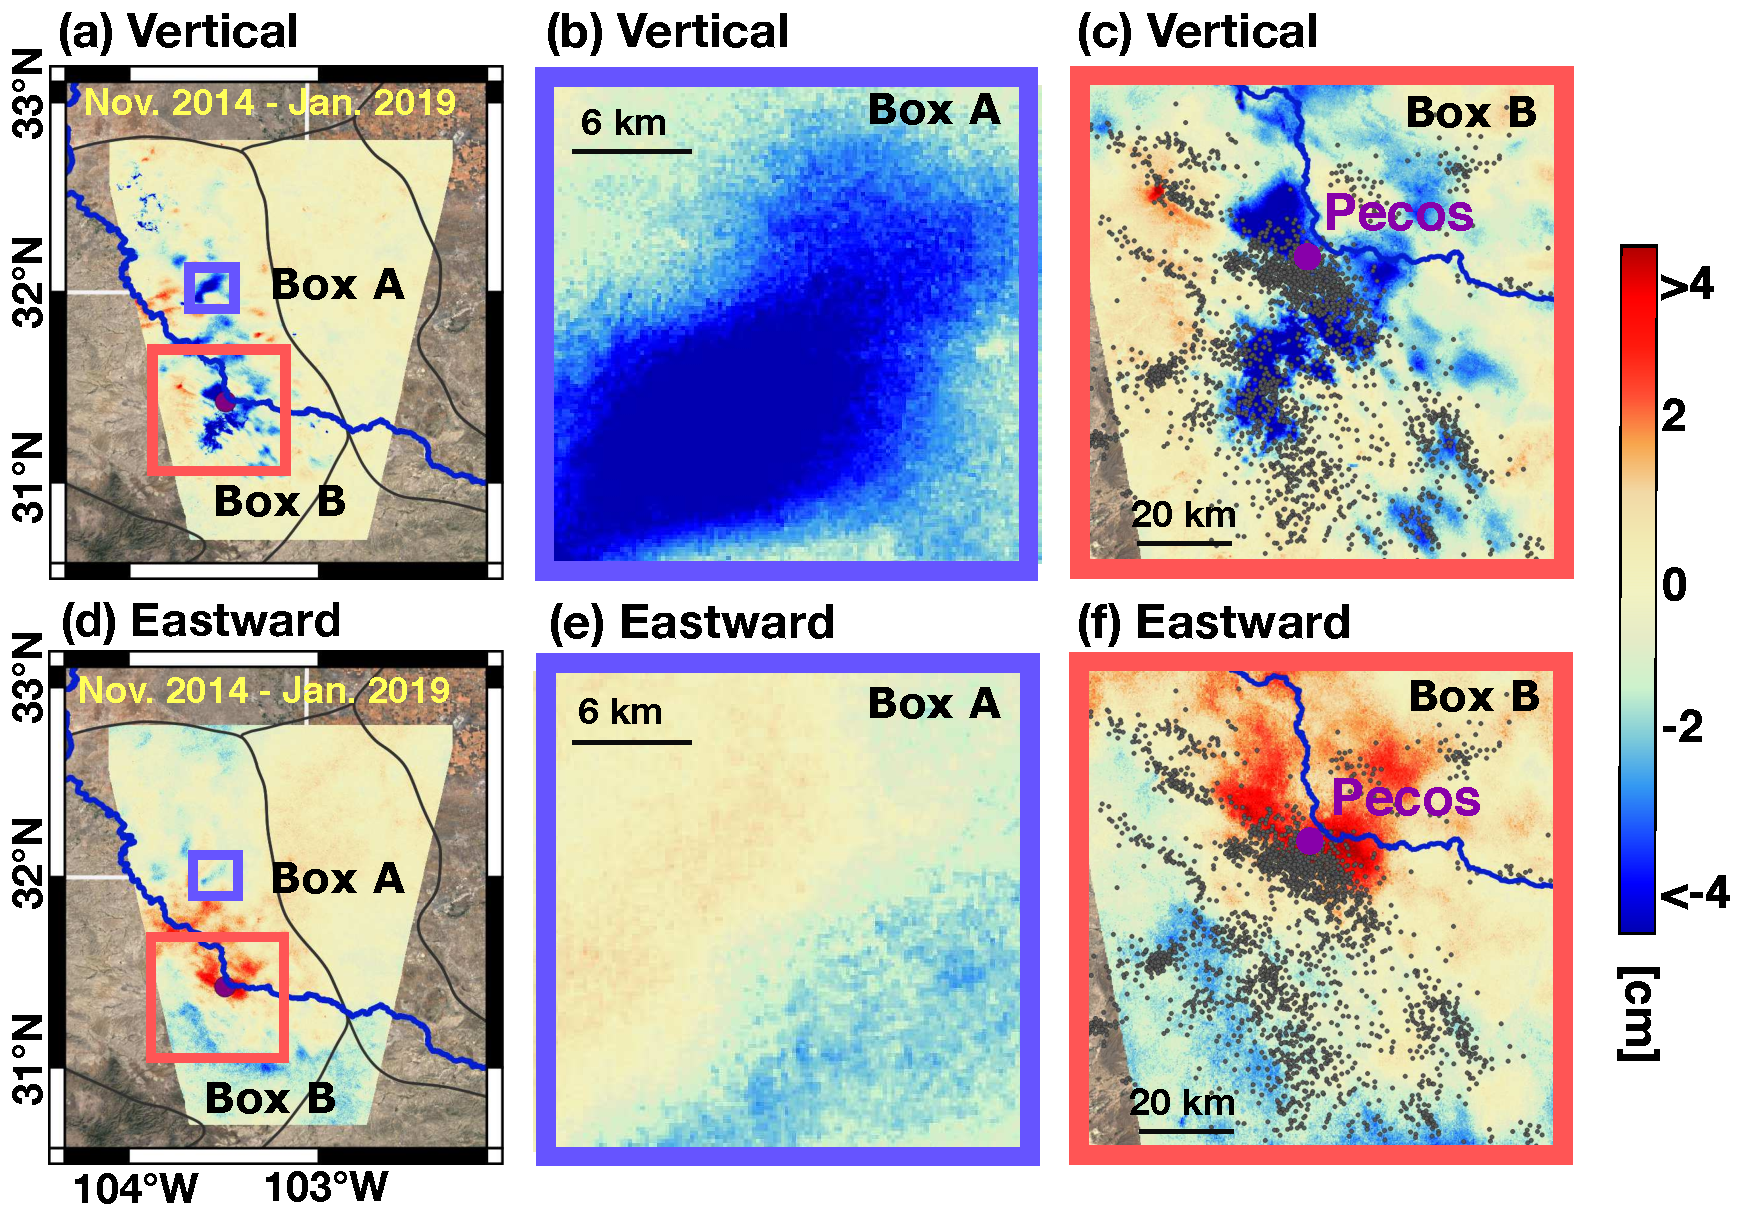
\includegraphics[width=0.96\linewidth]{figures/chapter4-grl/figure4-east-vertical-6panel-labelled-small.pdf}
	\caption[Cumulative vertical and horizontal deformation]{(a) Cumulative vertical deformation between Nov. 2014 and Jan. 2019 over the region where Sentinel-1 path 78 and path 85 overlap. A zoomed-in view of Box A in the northern Delaware Basin and Box B in the southern Delaware Basin are shown in panel (b) and (c) respectively. (d) Cumulative eastward deformation between Nov. 2014 and Jan. 2019 over the region where Sentinel-1 path 78 and path 85 overlap. A zoomed-in view of Box A in the northern Delaware Basin and Box B in the southern Delaware Basin are shown in panel (e) and (f) respectively. In the southern Delaware Basin, the observed vertical and eastward deformation (panel (c) and (f)) show linear patterns along with earthquake hypocenters (gray dots) detected by TexNet in 2018.}
	\label{fig:ch4-insar-decomp}
\end{figure}

\FloatBarrier

\section{Implications for geomechanical modeling}
Based on fault plane solutions derived from recent seismic activity and the faulting stress regime interpretations \citep{LundSnee2018StateStressPermian}, the Pecos area is in a normal faulting regime. We employed an elastic dislocation model \citep{Okada1992InternalDeformationDue} to demonstrate that the presence of dip-slip normal faults can produce the observed linear subsidence patterns in this area (Figure \ref{fig:ch4-model} (a)). We solved for the dip angle, depth, width along the dip direction, and slip magnitude of four normal faults by best fitting the forward model to InSAR vertical deformation observations, minimizing the sum of squared residuals, and maximizing the r-squared values \citep{Du1992ComparisonVariousInversion} (Appendix \ref{appen:okada}). The optimal solution suggests that the depth of the faults ranges from 0.9 km to 1.5 km, which is shallower than most of the TexNet recorded earthquakes (2-6 km in depth). Possible explanations for this discrepancy include: (1) the existence of aseismic fault slippage being responsible for the observed surface deformation \citep{McGarr2017WastewaterDisposalEarthquake}; (2) bias in earthquake depth estimation in the TexNet catalog \citep{Lomax2019ImprovingAbsoluteEarthquake}; (3) systematic modeling errors associated with representing a mechanically layered earth as a homogeneous half space \citep{Du1992ComparisonVariousInversion}. 



\begin{figure}
	\centering
	\includegraphics[width=\linewidth]{figures/chapter4-grl/figure5-modeling.pdf}
	\caption[Modeled surface deformation from fault slip and reservoir subsidence]{(a) InSAR-observed cumulative vertical deformation between Nov. 2014 and Jan. 2019 in the Pecos, TX area. (b) Modeled vertical deformation associated with four dip-slip faults. (c) Modeled vertical deformation associated with reservoir compaction. (d) Modeled total vertical deformation associated with four dip-slip faults and reservoir compaction (panel (b) $+$ panel (c)). (e) Difference between InSAR-observed and model-predicted vertical deformation (panel (a) $-$ panel (d)). (f) Difference between InSAR-observed and model-predicted vertical deformation along the B-B' transect.}
	\label{fig:ch4-model}
\end{figure}


After removing the best-fit deformation associated with dip-slip faulting (Figure \ref{fig:ch4-model} (b)), there is still $\sim$ 2 cm residual subsidence in the Pecos area (e.g. Figure \ref{fig:ch4-model} (f)). Given that shallow groundwater production was minimal in this region for the time period of interest \citep{Deng2020SurfaceDeformationInduced}, we introduced an elastic reservoir compaction model \cite{Geertsma1973LandSubsidenceCompacting} to our geomechanical analysis (Appendix \ref{appen:model-compact}). We implemented two layers of multiple cylindrical reservoirs corresponding to reported locations and depths of well clusters in the Delaware Mountain Group (DMG) and Wolfcamp reservoirs, which account for most of the recent oil and gas production in the region. We discretized the DMG layer based on a cluster of production wells predominantly perforated over a depth range of 1.5-1.8 km. The Wolfcamp wells are completed over a depth range of 3-3.6 km. We employed an objective function inversion method to solve for the reservoir pressure depletion pattern that best fit the InSAR-observed subsidence (Figure \ref{fig:ch4-model} (c)) \citep{Du2001PoroelasticReservoirModel}.

An important conclusion of this study is that both fault slip and reservoir inflation or compaction can produce observable surface deformation over an 80,000 square kilometer oil-producing region of the Permian Basin. The InSAR-observed subsidence patterns over the Pecos area can be modeled as slip over multiple faults and discretized cylindrical reservoir compaction (Figure \ref{fig:ch4-model} (d)-(f)). We note that InSAR subsidence data alone can constrain all pertinent fault and reservoir parameters in our normal faulting and reservoir compaction models. The InSAR observed cumulative surface deformation patterns, which show larger horizontal component than the model prediction, suggest that other factors, such as strike-slip faulting and heterogeneity in subsurface properties, may play a role. There have been extensive studies on how reservoir compaction and inflation as well as fault slippage alter stress fields in the subsurface and produce surface deformation \citep{Geertsma1973LandSubsidenceCompacting,Segall1992InducedStressesDue,Okada1992InternalDeformationDue,Du1992ComparisonVariousInversion,Vasco2005UseQuasiStatic,Vasco2008ReservoirMonitoringCharacterization,Khakim2012GeomechanicalModelingInsar}. InSAR surface deformation can be combined with this knowledge to evaluate fluid recovery efficiency and monitor disposal wells at low cost. Furthermore, these high-quality geodetic measurements are readily available to complement the TexNet seismic catalog for assessing the likelihood of fault motion and induced earthquake risks in Texas.




%(1) Algorithm
%(2) Time series result and validation
%(3) Deformation maps
%(4) Data now available for stakeholders, what people can do (brief discussion on Peter's work, we could use one of his figures I have).
%



\chapter{Robust Time Series Methods for Long-term Nonlinear Deformation}
\label{CHAP:5-robust-ts}


In this chapter, present a method for robustly extracting slow-moving cumulative surface deformation from time series with large noise. 
We perform a temporal smoothing using the robust LOcally WEighted Scatterplot Smoothing (LOWESS) regression technique \cite{Cleveland1979RobustLocallyWeighted} on noisy surface deformation time-series derived using SBAS.
%The method extends the ideas behind the outlier-removal technique presented in Chapter \ref{CHAP:4-GRL}.
Compared to the alternatives presenting in Section \ref{sec:ch4-method-compare}, the LOWESS smoothing more easily accounts for nonlinear deformation while also suppressing the 10-15 cm of tropospheric noise present in the summer SAR acquisitions. 
We demonstrate the technique using synthetic time series and using three paths of Sentinel-1 data over the Permian Basin in West Texas. 
The cumulative results show subtle basin-wide uplift features arising after 4-5 years of heavy sustained wastewater injection.



%- Problem: 
%1. Longer time series, the linear assumption becomes less valid.  This is at odds with the balance of using more measurements to average out tropospheric noise
%2. Methods incorporating temporal smoothness constraints (Find a few. e.g. Karissa? other temp smooth solvers...) or temp lienar filtering methods get influenced by strong tropo days. Even with smoothing, there are anomalous bumps 
%	- can get interpreted as deformation if we assume that all movements remaining after filtering are due to the low-pass deformation
%	

\section{Algorithm}
%	\bm{A \phi} = \bm{\Delta \phi} + \bm{\epsilon} . \label{eq:ch2-sbas-A}
%where  $\bm{A}$ is the system design matrix, and $ \bm{\epsilon}  $ is the vector of interferogram-specific noise sources (e.g. $ \Delta \phi_{decor}, \Delta \phi_{unwrap}, \Delta \phi_{scat}, \Delta \phi_{n} $ from Equation \eqref{eq:ch2-insar-noise-terms}).
Consider time series of LOS phase delay,  $ \bm{\phi} = \left[\phi_0, \phi_1, \ldots, \phi_{N-1} \right]^T $, for a single pixel solved using the SBAS system from Equation \eqref{eq:ch2-sbas-A}.
Here we consider the case that the interferogram-specific noise sources (e.g. $  \Delta \phi_{decor}, \Delta \phi_{unwrap}, \Delta \phi_{scat}  $) have been properly accounted for in the process used to calculate $ \bm{\phi} $.
Each element $\phi_i$ contains
% consists of all terms in Equation \eqref{eq:ch2-insar-noise-terms} which affect the phase of a SAR acquisition and all interferograms containing that acquisition
the deformation phase, $\frac{4 \pi}{\lambda} d_i$, as well as the atmospheric delay terms, $\frac{4 \pi}{\lambda} \alpha_i$.
Since deformation is usually the quantity of interest, there are several approaches to separating $ d_i $ from $ \alpha_i $.
If a functional model of deformation is known to exist (e.g. linear, transient jumps \citep{Chen20142010SlowSlip, Fielding2017SurfaceDeformationNorth}, seasonal variations \citep{Murray2018ShortLivedPause}, or a combination \citep{Riel2018QuantifyingGroundDeformation}), a model fit can be performed on the noisy $ \bm{\phi} $ time series to extract the model parameters of interest.
Alternatively, the authors of \cite{Berardino2002NewAlgorithmSurface} used spatial and temporal filters on $\bm{\Delta \phi}$, relying on the fact that the turbulent component of $\bm{\alpha}$ is uncorrelated in time \citep{Emardson2003NeutralAtmosphericDelay} while most deformation sources show strong temporal correlation.

%These filters are expanded upon and compared in Chapter \ref{CHAP:5-robust-ts}, where a new robust filter is presented to separate deformation from atmospheric noise.


\begin{figure}
\centering
%\includegraphics[width=.99\textwidth]{figures/chapter5-lowess/figure1-demo.pdf}
\caption[Demo of LOWESS fitting]{
	Demo of LOWESS fitting
	(a) fake time series to fit
	(b) weighting window
	(c) slope at one point
}
\label{fig:ch5-algo-demo}
\end{figure}


%
%%$ \bm{v} = (\bm{A}^T \bm{A})^{-1}\bm{A}^T \bm{\Delta \phi} $
%%As noted in \cite{Simons2007InterferometricSyntheticAperture}, 
%The least squares solution $ \bm{v} = (\bm{B}^T \bm{B})^{-1}\bm{B}^T \bm{\Delta \phi} $ (or minimum norm solution n $ \bm{v} = \bm{B}^{\dagger} \bm{\Delta \phi}$ ) from \cite{Berardino2002NewAlgorithmSurface} assume that all measurements in $\bm{\Delta \phi}$ have equal variance; subsequent authors have implemented a weighted least squares solution:
%\begin{equation}
%	%	\bm{\phi} = \bm{A}^{\dagger} \bm{\Delta \phi}
%	%	\bm{\phi} = (\bm{A}^T \bm{\Sigma}^{-1} \bm{A})^{-1}\bm{A}^T \bm{\Sigma}^{-1} \bm{\Delta \phi}  \label{eq:ch2-sbas-wls}
%	\bm{v} = (\bm{B}^T \bm{\Sigma}^{-1} \bm{B})^{-1}\bm{B}^T \bm{\Sigma}^{-1} \bm{\Delta \phi}  \label{eq:ch2-sbas-wls}
%\end{equation}
%where $ \bm{\Sigma} = \mathbb{E}[\bm{\epsilon} \bm{\epsilon}^T] $ is the measurement covariance matrix.




\begin{figure}
	\centering
%	\includegraphics[width=.99\textwidth]{figures/chapter5-lowess/figure1-demo.pdf}
	\caption[Effect of window size on LOWESS fit]{
		(a) Using a narrow window 
		(b) Using a wide window approaches a single linear fit
	}
	\label{fig:ch5-algo-window}
\end{figure}


\begin{figure}
	\centering
%	\includegraphics[width=.99\textwidth]{figures/chapter5-lowess/figure1-demo.pdf}
	\caption[Multiple iterations of LOWESS fit]{
		(a) First round fit at one $ x $ location (Same as Figure \ref{fig:ch5-algo-demo}c)
		(b) Additional weights imposed from the residuals of first fit
		(c) New weighting window
		(d) Improved fit from second and third iterations
	}
	\label{fig:ch5-algo-iteration}
\end{figure}


\section{Synthetic Example}



\begin{figure}
	\centering
%	\includegraphics[width=.99\textwidth]{figures/chapter5-lowess/figure1-demo.pdf}
	\caption[Multiple iterations of LOWESS fit]{
		(a) First round fit at one $ x $ location (Same as Figure \ref{fig:ch5-algo-demo}c)
		(b) Additional weights imposed from the residuals of first fit
		(c) New weighting window
		(d) Improved fit from second and third iterations
	}
	\label{fig:ch5-compare-tri}
\end{figure}



\section{InSAR Processing for Sentinel-1}

%For Sentinel-1 path 78, we processed all interferograms with temporal baselines less than 500. 
%Since all interferograms had less than 250 meter spatial baseline, we required no maximum spatial baseline threshold.  
%We unwrapped each interferogram using the Statistical-cost, Network-flow Algorithm for Phase Unwrapping (SNAPHU).
We use the Path 78 and Path 85 inteferograms from Section .
We reduce long wavelength and stratified tropospheric noise by removing a combined planar phase ramp and linear phase vs. elevation relation \cite{Doin2009CorrectionsStratifiedTropospheric, Zebker2021AccuracyModelFree}. We used the mean of the pixel values in a window around GPS station TXKM as a reference.
We repeated this process for descending path 85 and ascending path 151. Since path 151 does not contain station TXKM, or any other GPS station near the center of the acquisition, we used the referencing technique presented in \cite{Zebker2021AccuracyModelFree} to fit and remove a phase-elevation trend from all high-coherence pixels in each interferogram. This method relies on the assumption that most pixels in each interferogram do not show significant deformation, which is valid Path 151 which only partially overlaps with the western portion of the oil-producing Permian Basin. 
%our signals deform slowly over time

%FIGURE: 3 path study

%For each pixel, we solved for the cumulative line of sight path delay for all SAR acquisition dates using the SBAS linear system.
%The path delay consist of the true relative surface deformation on each date and a tropospheric noise component, which can lead to jumps of 10 cm or more between consecutive dates.
%Since the atmospheric noise is correlated in space but uncorrelated in time, previous authors have isolated and mitigated the atmospheric noise by using a high pass temporal filter followed by a 2D spatial low pass filter
%\cite{Ferretti2000NonlinearSubsidenceRate, Ferretti2001PermanentScatterersSar, Berardino2002NewAlgorithmSurface, Hooper2012RecentAdvancesSar}.
%Here we perform a temporal smoothing using the robust locally weighted regression (LOWESS) method \cite{Cleveland1979RobustLocallyWeighted}. For each pixel, LOWESS performs multiple iterations of weighted linear regression at each point in the time series. The method weights nearby points more heavily than far away points. We use a window size such that at least two years of SAR acquisitions are weighted for each date, with more points considered during times of regular acquisitions.
%Subsequent iterations use the residuals of the data points from the smoothed line to further deweight noisy acquisitions. Points with residuals larger than 6 times the median absolute residual are clipped to have 0 weight in future iterations. In this manner, the smoothing is robust to strong tropospheric turbulence noise that would otherwise leak into neighboring days using a moving average temporal filter. Additionally, since LOWESS assumes no underlying model, the smoothing can accommodate nonlinear deformation.
%
%To mitigate final residual long wavelength tropospheric noise, we remove quadratic ramp from the phase of each date in the time series (where we mask out pixels with $>$2 cm of estimated deformation to avoid removing deformation) \cite{Morishita2020LicsbasOpenSource}.

\section{Results}

\subsection{Permian Basin 7-year time series}

\subsection{GPS comparison}

\section{Discussion}

%1. Limitations of stacking to long time series
%2. Robust Time Series Methods
   %1. Regularization (Supplement from GRL)
   %2. LOWESS smoothing
%3. Synthetic Example
%4. 7 Year Time Series for the Permian Basin
%1. Comparison to GPS
%2. Anthropogenic Caused Deformation Patterns


%Problems with pixelwise uq
%- Image of blob, with 8 mm cutoff, question which part you trust and not
%- Leads into feature-wise uq







\chapter{Automatic Detection of InSAR Surface Deformation Signals In the Presence Severe Tropospheric Noise}
\label{CHAP:6-blob}
%In this chapter, we demonstrate methods for automatically detecting surface deformation signals in InSAR maps. We present a computer vision algorithm based on Laplacian of Gaussian filters. We show how the tropospheric noise levels can be estimated from InSAR data, and we use these estimates to simulate new instances of noise. We create confidence measures based on the simulations for automatically detected signals in real InSAR maps.


\section{Introduction}
\label{sec:ch6-intro}

Detection of surface deformation signals in maps derived from interferometric synthetic aperture radar (InSAR) poses a challenge due to the ubiquity of spatially correlated tropospheric turbulence noise. In this chapter,
we combine methods for tropospheric noise characterization with computer vision algorithms for detecting surface deformation.
We first present our computer vision algorithm, based on Laplacian of Gaussian (LoG) filtering, for finding signals of unknown size and location within InSAR deformation maps.
LoG-based detection algorithms were developed in the computer vision literature to detect repeatable image feature points at many scales \citep{Witkin1987ScaleSpaceFiltering, Lindeberg1998FeatureDetectionAutomatic}, and gained widespread use through the success of the Scale Invariant Feature Transform (SIFT) algorithm \citep{Lowe2004DistinctiveImageFeatures}. 
% for detecting surface deformation signals of unknown location and size in InSAR deformation maps. 
Additionally, we estimate expected magnitude of tropospheric artifacts in InSAR deformation maps by calculating the power spectral density of our study region's tropospheric noise and simulating many instances of similar noise.
We combine these two techniques to derive an empirical probability density function (PDF) of the size and magnitude of noise artifacts in our study region.
We demonstrate the performance of the algorithm on the two paths of Sentinel-1 data from Chapter \ref{CHAP:4-GRL} acquired between 2014 and 2019 over the oil-producing Permian Basin in West Texas. 
Several hundred deformation features are identified in areas known to contain clusters of oil production, wastewater injection, and seismic activity. 
%The algorithm detects many more features in both paths over time as 
%well on both paths of data, despite large variations in the strength of tropospheric noise between
We note that our algorithm detects surface deformation features caused by a wide variety of anthropogenic and natural causes despite requiring no prior physical models of the features of interest. Additionally, we generate confidences for each detected visual feature. Although we demonstrate the detection algorithm on cumulative deformation maps derived from stacking interferograms, it can be easily adapted to other types of multi-temporal InSAR time series methods.



%\section{Review of Automatic Deformation Detection for InSAR}

%With the launch of Sentinel-1, acquiring 250-km wide swaths of data every 6-12 days, several groups developed automated processing chains for producing regional or global databases of surface deformation using short-baseline interferograms.
%Several of these were applied to monitor volcano deformation \citep{Meyer2015IntegratingSarDerived, Valade2019TowardsGlobalVolcano, Lazecky2020LicsarAutomaticInsar}.
%Due to the large quantity of data, the early automatic detectors used pixel-wise metrics, such as changes to coherence \citep{Meyer2015IntegratingSarDerived}, thresholds on deformation velocity \citep{Raspini2018ContinuousSemiAutomatic, Bekaert2020InsarBasedDetection} or receiver operating characteristic cumulative sum control charts \citep{Albino2020AutomatedMethodsDetecting}. Other pixel-wise approaches have processed individual time series using dimensionality reduction or feature mapping mapping techniques, such as t-SNE \citep{Kerkhof2020IndividualScattererModel} or Long Short-term Memory Autoencoders (LSTM-AE) \citep{Ansari2021InsarDisplacementTime}, followed by density-based clustering algorithms.
%
%Classical machine learning approaches, such as principal component analysis (PCA) or independent component analysis (ICA), have also been exploited to separate deformation signal from noise \citep{Chaussard2014PredictabilityHydraulicHead, Ebmeier2016ApplicationIndependentComponent, Gaddes2018BlindSignalSeparation}. 
%These signal separation techniques may take entire deformation images as input, or may be performed pixel-wise on time series to cluster anomalous behaviors.
%Deep learning approaches using convolutional neural networks (CNNs) have been applied to automatically detect and localize features in InSAR deformation maps \citep{Anantrasirichai2018ApplicationMachineLearning, Anantrasirichai2019ApplicationConvolutionalNeural, Anantrasirichai2019DeepLearningApproach, Anantrasirichai2021DetectingGroundDeformation}.
%These efforts used large pretrained models, such as AlexNet \citep{Krizhevsky2012ImagenetClassificationDeep} or VGG19 \citep{Simonyan2014VeryDeepConvolutional}, that were adapted from RGB image classification benchmarks; this necessitated a pre-processing step of re-wrapping and/or colorizing the deformation maps to feed into the 3-channel RGB input. The models in \citep{Anantrasirichai2019DeepLearningApproach} were trained using labeled input data that was synthetically generated using noise and deformation models, in addition to the labeled real data from \citep{Anantrasirichai2018ApplicationMachineLearning}.
%CNN models were trained from scratch on synthetis data in \citep{Valade2019TowardsGlobalVolcano}
%to learn a decorrelation mask from input wrapped interferograms and detect volcanic ground deformation.  The authors in \citep{RouetLeduc2021AutonomousExtractionMillimeter} created a denoising autoencoder \citep{Vincent2008ExtractingComposingRobust}, also trained on synthetically generated data, which ingested 9 noisy patches of deformation time series maps and detected transient deformation based on an Okada fault model \citep{Okada1992InternalDeformationDue} or inflation/deflation from a Mogi point-source model \citep{Mogi1958RelationsEruptionsVarious}.
%
%
%Separate from the machine learning and computer vision work, several efforts have analyzed atmospheric noise levels in an attempt to yield a minimum-detectable deformation threshold.
%The earliest case of this was \citep{Emardson2003NeutralAtmosphericDelay}, who calculated an expected number of acquisitions needed to reliably detect some linear velocity given an atmospheric noise level $\sigma$. This work was extended to use external data sources.
%A Monte Carlo technique for generating pseudo-InSAR time series was developed in \citep{Barnhart2013CharacterizingEstimatingNoise}, which used sets of MODIS data over the same temporal range as the available SAR imagery.
%\citep{Parker2015SystematicAssessmentAtmospheric} used the North American Regional Reanalysis (NARR) weather model to produce estimates of atmospheric noise variance $\sigma$ on each SAR acquisition; similar to \citep{Emardson2003NeutralAtmosphericDelay}, these were propagated through a weighted least squares inversion to produce a pixel-wise uncertainty level on deformation velocities. \citep{Havazli2021DetectionThresholdEstimates} computes minimum deformation velocity thresholds based on the simulation of stratified and turbulent tropospheric noise. The authors simulate noise without deformation and compute expected ranges of residual tropospheric noise. The authors of, \citep{Havazli2021DetectionThresholdEstimates} that different study areas have different noise parameters, but do not present a way to estimate these noise levels directly from InSAR data, instead relying using MODIS PWV data to obtain a multiplier parameter for the strength of the stratified noise.
%

Interferometric Synthetic Aperture Radar (InSAR) has made it possible to monitor surface deformation with 10s–100s meter spatial resolution and millimeter-to-centimeter accuracy (e.g. \cite{Pritchard2004InSARbasedsurvey,  Chaussard2014PredictabilityHydraulicHead,  Chen20142010SlowSlip, Biggs2017GlobalVolcanoMonitoring, Chen2016ConfinedAquiferHead, Fielding2017SurfaceDeformationNorth, Chen2019TriggeringMw7.2}). Since the launch of the Sentinel-1 mission in 2014, the quantity and quality of open-access InSAR data has grown exponentially. Processing and interpreting such data often requires artificial intelligence and computer vision algorithms without extensive manual inspection. However, designing robust and scalable computer vision algorithms for automatic detection of InSAR surface deformation features is challenging. This is because InSAR measurement noise varies substantially in both space and time, and its magnitude is often comparable or larger than subtle deformation signals of interest. In particular, residual troposphere noise in InSAR surface deformation maps are spatially coherent, and it can often be visually mistaken as real surface deformation.


%(2) Paragraph 2: review existing work. I want a much shorter version than the one you sent to me, in a similar style like the RSE paper. Typically, we use 1-2 sentences for each major method (the key idea behind the algorithm and then what kind of demonstration they were able to do, we are not interested in methods without demonstration on real data). Maybe pick the most recent one and extend a little more details. Just focus on what they did, and not try to be a judge.

To address these challenges, previous studies developed algorithms for detecting deformation signals in pixel-wise InSAR deformation time series based on certain magnitude thresholds. The thresholds can be set manually \cite{Raspini2018ContinuousSemiAutomatic}, set using pixel-wise standard deviations \cite{Bekaert2020InsarBasedDetection}, derived from auxiliary data sources (e.g. global atmospheric weather models \cite{Parker2015SystematicAssessmentAtmospheric}, MODIS water vapor measurements \cite{Barnhart2013CharacterizingEstimatingNoise}), or derived from simulated noise parameters \cite{Havazli2021DetectionThresholdEstimates}. Principal component analysis (PCA) and independent component analysis (ICA) have also been used to explore decompositions of noisy time series data \cite{Chaussard2014PredictabilityHydraulicHead, Ebmeier2016ApplicationIndependentComponent, Gaddes2018BlindSignalSeparation}. Moreover, deep learning methods using convolutional neural networks (CNNs) have been applied to detect deformation features in individual interferograms \cite{Anantrasirichai2018ApplicationMachineLearning, Anantrasirichai2019ApplicationConvolutionalNeural} or InSAR time series \cite{RouetLeduc2021AutonomousExtractionMillimeter}. Because the detection problems are posed as a supervised learning task, they require either labeled training data \cite{Anantrasirichai2018ApplicationMachineLearning} or ground truth examples from simulated noise and deformation models \cite{Anantrasirichai2019DeepLearningApproach, RouetLeduc2021AutonomousExtractionMillimeter}. These supervised learning approaches work well when deformation signals of interest show spatial signatures that are distinct from InSAR measurement noise. In many applications, both deformation signals and tropospheric turbulence noise are spatially coherent ``blob-like'' features that look similar to human eyes.


%In many cases, the deformation signal may not be known beforehand, it is useful for automatic detectors to be sensitive to multiple classes of deformation signals. 
Automatic detection algorithms need to quantify the detection uncertainty based on the noise magnitude of a particular radar dataset. Auxiliary tropospheric data sources such as MODIS or weather models typically do not have sufficient spatial resolution to capture localized tropospheric turbulence noise at sub-kilometer scale. Here we present a new computer vision algorithm for detecting the size and location of unknown deformation features from a large volume of InSAR data. This algorithm is based on Laplacian of Gaussian (LoG) filters, which have been employed in the computer vision literature to detect repeatable image feature points at many scales (e.g. the Scale Invariant Feature Transform (SIFT) algorithm) \cite{Witkin1987ScaleSpaceFiltering, Lindeberg1998FeatureDetectionAutomatic, Lowe2004DistinctiveImageFeatures}. To determine whether a detected feature is associated with tropospheric artifacts, we estimate the tropospheric turbulence noise directly from InSAR data \cite{Tymofyeyeva2015MitigationAtmosphericPhase}. We analyze the tropospheric noise spectrum, and quantify the detection uncertainty based on tropospheric noise simulations that resemble the actual InSAR observations over the study area \cite{Hanssen2001RadarInterferometryData}.
%We use LoG filtering to detect features in simulated tropospheric noise maps and derive an empirical probability density function (PDF) of the size and magnitude of noise artifacts. We then use this PDF to calculate a false positive probability for each detected deformation in real InSAR maps over the same area. 
Our algorithm is flexible, and it can be integrated with different time series techniques to detect a broad range of deformation features.




\section{Methods}
\label{sec:methods}

\subsection{Automatic Feature Detection}
\label{subsec:methods-1-log}

Given a surface deformation map $M$ derived from InSAR data, the value $ M_{ij} $ at the $i^{th}$ row and $j^{th}$ column represents the magnitude of a cumulative, seasonal, or transient deformation signal at this pixel. Because the earth can be considered as a stratified elastic-viscoelastic medium, surface deformation features are often spatially coherent \cite{Segall2010EarthquakeVolcanoDeformation}. In this study, our goal is to automatically detect these features in an InSAR deformation map $M$ that covers a very large region (Algorithm 1).

There have been many computer vision algorithms that were designed to automatically detect spatially coherent ``blob-like'' features in 2D image data \cite{Lindeberg1993DetectingSalientBlob, Lindeberg1998FeatureDetectionAutomatic, Lowe2004DistinctiveImageFeatures}. In this study, we employ the Laplacian of Gaussian (LoG) filters as a blob detector. An LoG kernel $K^{(m)}$ with a size $\sigma_m$ is written as:
\begin{equation}
	K^{(m)}_{ij} = \left(\frac{(i - l)^2 + (j - l)^2 - 2\sigma_m^2}{2 \pi \sigma_m^4}\right) \, e^{-\frac{ (i - l)^2 + (j - l)^2}{2 \sigma_m^2}} \label{eq:log-kernel}
\end{equation}
where pixel indices $ij  \in \left\lbrace 0, 1, \ldots, 2l \right\rbrace$. The unit of $\sigma_m$ is given in pixels, which can be scaled to meters based on the pixel spacing of the InSAR deformation map $M$.



\begin{figure}
	\centering
	\includegraphics[width=0.59\linewidth]{figures/chapter6-blobs/figure1_log_examples.pdf}
	\caption{
		Laplacian of Gaussian (LoG) kernels with (a) $\sigma_m=30$ pixels and (b) $\sigma_m=80$ pixels for an image of size of 500-by-500 pixels.
	}
	\label{fig:log-kernel}
	%
\end{figure}



We generate a set of LoG kernels $K^{(1)}, K^{(2)}, \ldots$ with progressively larger $\sigma_m$ (Figure \ref{fig:log-kernel}), and calculate the $m^{th}$ filter response $ L^{(m)} $ as:
\begin{equation}
	L^{(m)} = M \ast K^{(m)}  \label{eq:log-layer-conv}
\end{equation}
%However, this operation is computationally expensive for larger kernels; thus, the filtering is carried out in the Fourier domain.
Here $*$ denotes the 2D discrete convolution, which is typically computed using the Fast Fourier Transform (FFT) algorithm because of its superior computational efficiency \cite{Szeliski2022ComputerVision}.



\begin{figure}
	\centering
	\includegraphics[width=0.59\linewidth]{figures/chapter6-blobs/figure2_log_response.pdf}
	\caption{
		(a) A synthetic deformation map that contains one Gaussian-shaped uplift feature in the upper left and one elliptical Gaussian subsidence feature in the lower right. (b) LoG response amplitudes for 20 filters with various sizes ($\sigma_m$) at three marker points. The marker locations are shown in panel (a). (c)-(e) The LoG filter responses for $\sigma_m=$ 12, 50, and 84.}
	\label{fig:log-response}
	%
\end{figure}


To demonstrate how to estimate the size of an unknown deformation feature from the filter responses, Figure \ref{fig:log-response} (a) shows a $500 \times 500$ synthetic deformation map $M$ that contains one Gaussian-shaped uplift feature in the upper left and one elliptical Gaussian subsidence feature in the lower right. We filtered this deformation map using 20 LoG kernels of sizes ranging from $\sigma_1 = 3$ pixels to $\sigma_{20} = 100$ pixels with a base-2 logarithmic spacing, and the filter responses are shown in Figure \ref{fig:log-response} (b)-(e). For the round uplift case, the filter response $L^{(m)}$ (the black curve in Figure \ref{fig:log-response} (b)) is strongest when the kernel size $\sigma_m$ matches the deformation feature radius $r$ as $r = \sqrt{2}\sigma_m$. This is known as the extreme point, or the local maximum points of $|L^{(m)}|$ for all attempted $\sigma_m$. For the elliptical subsidence case, the extreme point is reached when the average length of the two primary axes of the deformation feature is $\sim \sqrt{2}\sigma_m$ (the green curve in Figure \ref{fig:log-response} (b)). For the case of no deformation, no substantial filter response is generated for any filter size (the gold curve in Figure \ref{fig:log-response} (b)).



In the case that two candidate blobs have more than 50\% overlapping area, the blob with a smaller size is discarded. 
Additionally, the LoG filter may falsely flag ghost blobs at the edges of real deformation features. This is because deformation features with strong curvature at the center also contain a strong opposite-signed curvature near the border \cite{Lindeberg1998FeatureDetectionAutomatic}. To remove those false positives, we use the distance from the candidate blob's center location to the nearest deformation amplitude extremum as a measure. If this distance is close to the blob radius, the detection is likely a ghost blob. In our test case, we discarded blobs with local extremum distances larger than 75$\%$ of the blob radius, which effectively removed all visible false positives near the edge of real deformation features.

For the $k^{th}$ detected deformation feature, our algorithm outputs the blob center location $(i_k, j_k)$, the blob radius $ r_k$, the filter response magnitude $|g_k|$ at the extreme point, and the deformation magnitude $|\bar{d_k}|$ defined as the weighed maximum of all pixels within the $k^{th}$ blob:
\begin{equation}
	\bar{d_k} = \max_{kk} |w_{kk} M_{kk} | 
\end{equation}
Here the weight $w_{kk}$ equals $\exp\left[-(r_{kk} / r_k)^2\right]$, where $r_{kk}$ is the distance between a pixel within the blob and the blob center. The exponential weighting prevents pixel outliers from distorting the measure of feature magnitude. 

We can exclude undesired deformation features by setting magnitude thresholds on $|g_k|$ and $|\bar{d_k}|$ based on users' interest. Furthermore, we need to determine whether a detected deformation feature has a signal magnitude above the noise level of the InSAR deformation map, which is the focus of the following method sections. 


\begin{algorithm}
	\caption{LoG Based Deformation Feature Detection}\label{algo:blobs}
	\SetAlgoLined
	\KwIn{2D InSAR deformation map $M$}
	\KwResult{For each $k \in {1, \ldots, N_d}$ detections, the algorithm outputs the blob center location $ (i_k,j_k) $, the blob radius $ r_k $, the filter response magnitude $|g_k|$ at the extreme point, the deformation magnitude $|\bar{d_k}|$ }
	
	
	// Calculate filter responses:\\
	\ForEach{$ \sigma_m \in \left\lbrace \sigma_{min} \ldots \sigma_{max}\right\rbrace $}{
		%$L^{(n)} = \mathcal{F}^{-1} \left[ \mathcal{F} M \cdot  \mathcal{F} K^{(n)} \right] $
		$ L^{(m)} = M \ast K^{(m)}  $
		%$\nabla^2_{norm} L(\cdot, \cdot, \sigma) \gets I(\cdot, \cdot) * \nabla^2_{norm} G(\cdot,\cdot, \sigma)$
	}
	
	// Find candidate blobs from local extrema:\\
	\For{$ (i, j, m) \in  L $}{
		\If{$L[i, j, m] $ is local extremum }{
			% \If{$\det \mathcal{H}_{norm} L(x,y,\sigma ) $ is local extremum }{
				Compute $ r = \sqrt{2}\sigma_m $ \\
				Add $ (i, j, r) $ to list of candidate detections
		}
	}
	// Prune blobs with overlap:\\
	\ForEach{$ b_1 := (i_1, j_1, r_1), b2 := (i_2, j_2, r_2) \in $ candidates}{
		%	Form circle of radius $ r_i $ around $ (i_1, j_1) $\\
		\If{ Overlap$( b_1, b_2 ) > 0.5 $  }{
			Remove smaller of $ b_1, b_2 $
		}
	}
	
	// Prune edge blob false positives:\\
	\ForEach{$ b_k := (i_k, j_k, \sigma_k) \in $ candidates}{
		Find coordinates $(u, v)$ of local max of $M$ within
		radius $r_k$ around $ (i_k, j_k) $
		\\
		\If{ $\sqrt{(x - u)^2 + (y - v)^2} > 0.75 $  }{
			Discard $ b_k $
		}
	}
	// Prune with thresholds $ \gamma_g, \gamma_d $:\\
	\ForEach{$ b_k := (i_k, j_k, r_k,|g_k|, |\bar{d_k}|) \in $ candidates}{
		\If{ $ |g_k| <  \gamma_g $ \text{or} $ |\bar{d_k}| <  \gamma_d $  }{
			Discard $ b_k $
		}
	}
\end{algorithm}



\subsection{Tropospheric Noise Spectrum}
\label{subsec:methods-2-tropo-spectrum}
InSAR measurement noise can also produce spatially coherent "blob-like" features that are detectable by our algorithm.  Here we focus on characterizing the tropospheric turbulence noise in each SAR scene. This is because tropospheric turbulent noise (1) is correlated in space \cite{Emardson2003NeutralAtmosphericDelay, Lohman2005SomeThoughtsUse}; (2) is present in all InSAR data sets with greatly varying magnitudes \cite{Barnhart2013CharacterizingEstimatingNoise, Hooper2012RecentAdvancesSar}; and (3) is often the primary noise source that limits InSAR measurement accuracy \cite{Jolivet2014ImprovingInsarGeodesy, Bekaert2015StatisticalComparisonInsar, Parker2015SystematicAssessmentAtmospheric}.

Consider an interferogram formed using two SAR scenes acquired at times $t_1$ and $t_2$. In the case that tropospheric turbulence noise is the dominant noise term, the measured interferometric phase $\phi_{1,2}$ (in radians) at a pixel of interest can be written as \cite{Zebker1997AtmosphericEffectsInterferometric}:
\begin{equation}
	\phi_{1,2} \approx \frac{4 \pi}{\lambda} \left(\alpha_2 - \alpha_1 + \Delta d_{1,2} \right)
\end{equation}
where $ \lambda $ is the radar wavelength, $\alpha_1$ and $\alpha_2$ represent the tropospheric delay at the two SAR acquisition times $t_1$ and $t_2$, and $\Delta d_{1,2} $ is the Line-Of-Sight (LOS) deformation ($d_2-d_1$) between $t_1$ and $t_2$. The unit of $\lambda$, $\alpha_1$, $\alpha_2$, and $\Delta d_{1,2} $ is in centimeters. 

Given $N$ SAR acquisitions, we can estimate the tropospheric noise on the $n^{th}$ SAR acquisition date by averaging $N-1$ interferograms that share the common reference SAR scene $n$ \cite{Tymofyeyeva2015MitigationAtmosphericPhase}:
%multline not needed for single column
%\begin{multline}
%\bar{\alpha}_n = \frac{\lambda}{4 \pi} \frac{1}{N-1} \left(\sum_{k=1, k \neq n}^{N} \phi_{k,n}\right)  \\
%=  \alpha_n  + \frac{1}{N-1} \left( \sum_{k=1, k \neq n}^{N}  \Delta d_{k,n} - \sum_{k=1, k \neq n}^{N}  \alpha_k  \right)  \label{eq:avg-ifg} 
%\end{multline}
\begin{equation}
	\bar{\alpha}_n = \frac{\lambda}{4 \pi} \frac{1}{N-1} \left(\sum_{k=1, k \neq n}^{N} \phi_{k,n}\right)  
	=  \alpha_n  + \frac{1}{N-1} \left( \sum_{k=1, k \neq n}^{N}  \Delta d_{k,n} - \sum_{k=1, k \neq n}^{N}  \alpha_k  \right)  \label{eq:avg-ifg} 
\end{equation}
Because tropospheric turbulence noise is uncorrelated in time for scales longer than one day \cite{Emardson2003NeutralAtmosphericDelay, Onn2006ModelingWaterVapor}, the term $ \frac{1}{N-1} \sum \alpha_k \rightarrow 0$ when $N$ is sufficiently large. 
Under the assumption that $ \frac{1}{N-1} \sum \Delta d_{k,n} $ is relatively small comparing to $\alpha_n$, we compute $ \bar{\alpha}_n $ at each pixel to obtain a tropospheric turbulence noise map $A^{(n)}$ for the $n^{th}$ SAR acquisition date over the entire study area. In Section \ref{sec:results:path78}, we further discuss the impact of the deformation signals on our tropospheric noise analysis.


We next compute the 2D Power Spectral Density (PSD) of the $n^{th}$ tropospheric noise estimates at  wavenumber $ k_x, k_y $ (with units $1/m$) as \cite{Jacobs2017QuantitativeCharacterizationSurface}:
\begin{equation}
	\text{PSD}_n(k_x, k_y) = \frac{| \widehat{A^{(n)}} |^2 }{N_x N_y (\frac{1}{\Delta x \Delta y}) } \label{eq:pow-spec}
\end{equation}
where  $\widehat{A^{(n)}}$ is the Discrete Fourier transform (DFT) of  the $n^{th}$ tropospheric noise map $A^{(n)}$, $\Delta x$ and $\Delta y$ are the interferogram pixel spacings (in meters) in the $x$ and $y$ directions, $N_x$ and $N_y$ are the total number of pixels in the $x$ and $y$ directions, and the squared absolute value and division are pixel-wise operations. 


As an example, Figure \ref{fig:psd-example} (a) shows a synthetic 2D tropospheric turbulence noise map. We calculate the 2D PSD of the noise map following Equation \eqref{eq:pow-spec} (Figure \ref{fig:psd-example} (b)). Under the assumption that tropospheric noise is isotropic, we average all pixels with a distance  $k= \sqrt{k_x^2 + k_y^2}$ from the origin to generate a 1D PSD as a function of $k$ \cite{Hanssen2001RadarInterferometryData}.
We plot the 1D PSD on a log-log scale, which rolls off following a power law at higher frequencies (Figure \ref{fig:psd-example} (c)). By contrast, the power spectrum of spatially uncorrelated while noise is relatively flat across all frequencies $k$ (Figure \ref{fig:psd-example} (d)-(f)).


\begin{figure}
	\centering 
	\includegraphics[width=0.59\linewidth]{figures/chapter6-blobs/figure3_psd_radial.pdf}
	%\includegraphics[width=0.98\linewidth]{figures/chapter6-blobs/figure3_psd_radial.png}
	\caption{
		(a) A simulated 2D turbulent atmospheric noise map with $ 500 \times 500 $ pixels at $100$ meter pixel spacing.
		(b) 2D Power Spectral Density (PSD) of the tropospheric noise map in panel (a).
		(c) 1D PSD as a function of wavenumber $k = \sqrt{k_x^2 + k_y^2}$, under the assumption that tropospheric noise is isotropic.
		(d) A simulated 2D white noise map (spatially uncorrelated) with the same dimension and pixel spacing as panel (a)
		(e) 2D PSD of the white noise map in panel (d).
		(f) 1D PSD as as a function of wavenumber $k = \sqrt{k_x^2 + k_y^2}$. Here We averaged the 1D PSD of 50 2D white noise instances to improve the statistical stability of the spectral estimates.
	}
	\label{fig:psd-example}
\end{figure}


\subsection{Uncertainty Quantification}
\label{subsec:methods-3-noise-sim}

Using the average 1D PSD of all $N$ InSAR-observed tropospheric turbulence noise maps, we can simulate $N$ 2D noise incidences  $S^{(1)},\dots, S^{(N)} $ that closely resemble the real tropospheric noise over the study area \cite{Hanssen2001RadarInterferometryData}. Using these simulated noise maps, we form up to $N(N-1)/2$ noise-only interferograms, and derive a time series solution following the same method for generating the real InSAR deformation map $M$ (e.g. \cite{Sandwell1998PhaseGradientApproach, Berardino2002NewAlgorithmSurface}). Because these synthetic interferograms contain no deformation, any "blob-like" features in the simulated time series solution are associated with tropospheric noise. We record the radius $r_k$,  the filter response magnitude $|g_k|$ and the magnitude $|\bar{d_k}|$ of each noise feature using our automatic blob detection algorithm.

Similarly, we generate many synthetic InSAR data sets that share the same noise spectrum derived from data, and record all detected noise blobs. We create 2D histograms of the noise attributes (filter response magnitude vs. radius and deformation magnitude vs. radius), which allows us to remove candidate blob features in the real deformation map $M$ that are likely due to tropospheric noise artifacts.


\section{Test Site and Available InSAR Data}
\label{sec:site}

We tested our deformation detection algorithm on over an 80,000 km$^2$ oil-producing region in the Permian Basin, West Texas.  As described in \cite{Staniewicz2020InsarRevealsComplex}, we processed 84 ascending Sentinel-1 scenes (Path 78, Frames 94–104) acquired between November 2014 and January 2019 (Figure \ref{fig:study-area}). We imposed no maximum spatial baseline and a maximum temporal baseline of 800 days for interferogram selection, resulting in 2550 multi-looked interferograms with 120 m pixel spacing.  We used the GPS station TXKM as the reference location, where little surface deformation was observed over the study period (Figure \ref{fig:study-area}, yellow dot).



\begin{figure}[hbt!]
	\centering
	\includegraphics[width=0.59\linewidth]{figures/chapter6-blobs/figure4-study-area.pdf}
	%\includegraphics[width=0.96\linewidth]{figures/chapter6-blobs/figure4-study-area.png}
	\caption{GPS and InSAR data coverage over the Permian Basin. Teal and red boxes indicate Sentinel-1 InSAR coverage for ascending Path 78 and descending Path 85. GPS station TXKM (yellow dot) was used as the reference point for both paths.
		%Each path contains over 80 SAR acquisitions, leading to over 3500 interferograms per path at 180 m pixel spacing.
	}
	\label{fig:study-area}
\end{figure}




We employed a stacking approach \cite{Sandwell1998PhaseGradientApproach, Staniewicz2020InsarRevealsComplex} to calculate the average LOS velocity $v_{avg}$ at each ground pixel over a time period of interest $ T $ as
\begin{equation}
	v_{avg} = \frac{\sum_{i \in G} \Delta d_i}{\sum_{i \in G} t_i}
	\label{eq:ch6-stacking}
\end{equation}
where $G$ is a subset of interferograms formed using two SAR scenes acquired within the time period $T$. The LOS measurement (in cm) and the temporal baseline of the $i^{th}$ interferogram in $G$ are written as $\Delta d_i$ and $ t_i $ respectively.
In this study, we used 29 SAR scenes acquired between November 2014 and January 2017 to solve for the average velocity during this period, and we computed the cumulative deformation as the average velocity times the total time span ($\sim 2$ years). Similarly, we used 52 SAR scenes acquired between November 2014 and January 2018, and 84 SAR scenes acquired between November 2014 to January 2019 to derive the cumulative deformation maps over these two study periods ($\sim 3$ and $4$ years).

We estimated the tropospheric turbulence noise for each SAR acquisition date using all interferograms that contain this SAR scene based on Equation \eqref{eq:avg-ifg}. We removed a quadratic ramp in each noise map, and calculated the average 1D PSD of all 84 noise maps as described in \ref{subsec:methods-2-tropo-spectrum}.
Using the average noise spectrum, we generated 29 synthetic noise maps, which corresponds to the 29 Sentinel-1 acquisition dates between November 2014 and January 2017. We formed noise-only synthetic interferograms and calculated the cumulative stacking solution using Equation \eqref{eq:ch6-stacking}. We ran our blob detection algorithm on the noise-only stacking solution, and recorded the size, the filter response magnitude, and the magnitude of each noise blob feature. We repeated this process until the number of recorded detections exceeded 100,000. We smoothed the resulting histograms using a kernel density estimate (KDE) \cite{Scott2015MultivariateDensityEstimation}, and generated 2D empirical Probability Density Functions (PDFs) of the noise attributes for the November 2014-January 2018 cumulative LOS deformation map.
Similarly, we ran additional simulations to generate 2D histograms of the noise attributes for the November 2014-January 2018, and November 2014-January 2019 cumulative deformation maps.
These histograms were then used to remove candidate blob features in the real Sentinel-1 InSAR deformation maps that are likely due to tropospheric noise artifacts.

We also processed 81 descending Sentinel-1 scenes (Path 85 Frames 483–493) acquired between November 2014 and January 2019 (Figure \ref{fig:study-area}). The same GPS station TXKM was used as the reference location to calibrate all interferograms. Following the same processing strategy, we estimated three cumulative deformation maps spanning November 2014 to January 2017, January 2018, and January 2019. We characterized the tropospheric noise from InSAR data, and identified deformation features in the cumulative deformation maps that are likely real.



\section{Results and Discussion}
\subsection{Path 78 detections}
\label{sec:results:path78}
%\subsection{Tropospheric Noise Power Spectra}
Figure \ref{fig:results-noise} (a)-(c) shows three estimated tropospheric noise maps for Sentinel-1 ascending Path 78 acquisitions 2017-12-12, 2018-09-14, and 2017-06-15. We observe blob-like turbulence features ranging from a few kilometers up to tens of kilometers in diameter, and the magnitude of the tropospheric turbulence noise varies substantially on different days (Figure \ref{fig:results-noise} (d)). For example, the maximum absolute tropospheric noise observed on 2017-12-12, 2018-09-14, and 2017-06-15 are 1.8 cm, 3.2 cm, and 12.6 cm, respectively. Overall, $\sim$ 50\% of Path 78 scenes were acquired in quiet atmospheric conditions with a maximum noise level under 4 cm. Approximately, 35\% scenes were acquired in moderate turbulence conditions (a maximum noise level of 4-10 cm), and 15\% scenes were acquired in strong turbulent noise conditions (a maximum noise level of 11-15 cm). 

Because InSAR phases are measured with respect to a reference point, we calculated tropospheric noise estimates relative to the center of the map (the noise reference point). We plotted the mean absolute tropospheric noise vs. distance to the noise reference point (Figure \ref{fig:results-noise}(e)). For the majority of the Path 78 acquisitions, tropospheric turbulent noise increases as the square root of the distance for the first $\sim 50$ km, and then the magnitude of the tropopsheric noise does not change much as the distance increases. This means that the tropospheric noise is spatially correlated with a correlation length of $\sim 50$ km, and the tropospheric noise magnitude over the flat portion of the curve is a measure of the noise activity level. 



\begin{figure*}
	\centering 
	%	\includegraphics[width=0.98\linewidth]{figures/chapter6-blobs/figure5_noise_path78.png}
	\includegraphics[width=0.98\linewidth]{figures/chapter6-blobs/figure5_noise_path78.pdf}
	\caption{
		InSAR-estimated tropospheric turbulence noise maps for three Path 78 SAR acquisitions: (a) 2017-12-12 (up to 1.8 cm noise), (b) 2018-09-14 (up to 3.2 cm noise), and (c) 2017-06-15  (up to 12.6 cm noise).
		(d) The distribution of peak tropospheric noise magnitude (in centimeters), (e) the root mean squared value of tropospheric noise vs. distance from the center of the map, and (f) the estimated 1D PSDs for 84 Sentinel-1 Path 78 acquisitions used in this study. In panel (e) and (f), the color lines represent three SAR acquisitions (panel (a)-(c)) with different tropospheric noise levels. The black line in panel (f) represents the mean PSD of all 84 acquisitions.}
	\label{fig:results-noise}
\end{figure*}


The 1D PSDs for the 84 tropospheric turbulence noise maps give an alternative view of the distribution of noise power over different frequencies (Figure \ref{fig:results-noise} (f). For most spatial frequencies, the PSDs decay following the -8/3 power law described in previous studies \cite{Hanssen2001RadarInterferometryData, Onn2006ModelingWaterVapor}. This slope flattens at the low frequencies because we removed the quadratic phase in the noise solutions. The slope also flattens at high frequencies, where decorrelation noise introduces pixel-level variations in the noise map.
%\subsection{Simulated tropospheric turbulence noise and Uncertainty Quantification}



\begin{figure*}
	\centering 
	%\includegraphics[width=0.98\linewidth]{figures/chapter6-blobs/figure_results_simulation_kde.png}
	\includegraphics[width=0.9\linewidth]{figures/chapter6-blobs/figure_results_kde.pdf}
	\caption{ (a)-(c) Log Probability Density Function (PDF) of detecting tropospheric noise blobs as a function of feature size $r$ and filter response magnitude $|g|$ for three cumulative LOS deformation maps: November 2014 - January 2017 (29 SAR scenes from Path 78), November 2014 - January 2018 (52 SAR Scenes from Path 78), and November 2014 - January 2019 (84 SAR Scenes from Path 78).
		(d)-(f) Log Probability Density Function (PDF) of detecting tropospheric noise blobs as a function of feature size $r$ and deformation magnitude $|d|$ for the same three cumulative LOS deformation maps.
		The PDFs were generated from 2D histograms using a kernel density estimate (KDE) \cite{Scott2015MultivariateDensityEstimation}.
	}
	\label{fig:results-kde}
\end{figure*}

Using the mean 1D PSD shown in Figure \ref{fig:results-noise} (f), we simulated instances of tropospheric turbulence, and computed the empirical PDFs of the noise attributes for each deformation map (Figure \ref{fig:results-kde}).  Most of detected noise features have small radii ($r <$ 5 km). For the 29 SAR acquisition case, the noise features are unlikely to be larger 2 cm in magnitude or have a filter response stronger than 0.7 (Figure \ref{fig:results-kde} (a), (d)). For the 52 SAR acquisition case, the noise features are unlikely to be larger 1.5 cm in magnitude or have a filter response stronger than 0.6 (Figure \ref{fig:results-kde} (b), (e)). For the 84 SAR acquisition case, the noise features are unlikely to be larger 1.2 cm in magnitude or have a filter response stronger than 0.5 (Figure \ref{fig:results-kde} (c), (f)).
%(Figure \ref{fig:results-kde}(a-c)). The noise instances are spatially isotropic and contain many $\sim$3 cm blob-like features ranging from several km up to $\sim$100 km in length. As outlined in Section \ref{sec:site}, we computed three LOS deformation maps from 29,52, and 84 noise instances, and we recorded all detected noise features. The resulting histograms of ($g$ vs. $r$ and $\bar{d}$ vs. $r$) were smoothed using a kernel density estimate (KDE) \cite{Scott2015MultivariateDensityEstimation} to create 2D empirical probability density functions (PDFs) (Figure \ref{fig:results-kde}). As the number of SAR acquisitions increases to 52 (Figure \ref{fig:results-kde}(b),(e)) and 84 (Figure \ref{fig:results-kde}(c),(f)), the amplitudes of detected noise features decreases for all $r$.
Note that the maximum and minimum sizes of detected features in Figure \ref{fig:results-kde} (d)-(f) are determined by the choice of maximum and minimum kernel sizes $\sigma_{max}$ and $\sigma_{max}$ in our automatic detection algorithm. By imposing the prior knowledge that oil and gas-production related deformation bowls are unlikely to be larger than 30-40 km in the Permian Basin \cite{Staniewicz2020InsarRevealsComplex}, $\sigma_{max}$ was set so that the maximum detected feature radius $r$ was approximately 20 km. Thus, large-scale tropospheric noise features ($>$ 20 km) were not recorded in the noise simulations.
%\subsection{West Texas Detected Deformation}



\begin{figure*}
	\centering 
	%\includegraphics[width=0.98\linewidth]{figures/chapter6-blobs/figure_results_detections_vert.png}
	%\includegraphics[width=0.98\linewidth]{figures/chapter6-blobs/figure_results_blobs_path78.png}
	\includegraphics[width=0.98\linewidth]{figures/chapter6-blobs/figure_results_blobs_path78.pdf}
	\caption{
		Detected deformation features (gray circles) from the three Path 78 cumulative LOS deformation maps. Features with more than 5\% chance of being noise for their radius, according to either the filter magnitude or image magnitude PDFs (Figure \ref{fig:results-kde}), have been removed. Green lines correspond the boundaries of the Delaware Basin, Central Basin Platform, and Midland Basin from west to east.
		% Not shown are features which, given their radius, have with more than 5\% chance of being noise according to either the filter magnitude or image magnitude PDFs (Figure \ref{fig:results-kde}). 
	}
	\label{fig:results-detections}
\end{figure*}


Using the empirical PDFs of the noise attributes, we removed detections with more than 5\% chance of being noise from three Path 78 cumulative deformation maps (Figure \ref{fig:results-detections}). We identified 57 deformation features in the Nov. 2014-Jan. 2017 cumulative deformation map, 147 features in the Nov. 2014-Jan. 2018 map, and 268 features in the Nov. 2014-Jan. 2019 map. The increasing number of detected deformation features is due to (1) the oil and gas production rate experienced a sharp rise over the study period \cite{Staniewicz2020InsarRevealsComplex}; and (2) a larger number of SAR acquisitions reduces the noise level in the InSAR cumulative deformation solutions.



The detected features are mainly clustered in regions within the Midland Basin and the Delaware Basin. Here oil production and wasterwater injection caused many centimeter-level subsidence and uplift features. In the Southern Delaware Basin, the observed linear deformation features parallel the inferred favorable fault plane orientation proposed by \cite{LundSnee2018StateStressPermian}, and they align with a cluster of recent shallow earthquakes cataloged by TexNet \cite{Savvaidis2019TexnetStatewideSeismological}. Very few deformation features were detected in the Central Basin Platform, where oil and gas are mostly produced from conventional reservoirs and the subsurface pressure was well maintained.


\begin{figure*}
	\centering 
	% vertical version:
	\includegraphics[width=0.98\linewidth]{figures/chapter6-blobs/figure_discussion_residual_defo.pdf}
	%\includegraphics[width=0.98\linewidth]{figures/chapter6-blobs/figure_discussion_residual_defo_horizontal.pdf}
	\caption{
		(a) InSAR-estimated tropospheric noise map for the Path 78 SAR acquisition 2018-09-14. 
		(b) Cumulative LOS deformation from Nov. 2014 to Jan. 2019 as inferred from Sentinel-1 Path 78 InSAR data.
		(c) 1D PSDs derived from the tropospheric noise map (black) and the tropospheric noise plus deformation map (red).
	}
	\label{fig:discussion-residual-defo}
\end{figure*}


For the West Texas case, the residual deformation term $  \frac{1}{N-1}  \sum  \Delta d_{n,k} $ in Equation \eqref{eq:avg-ifg} does not significantly influence our noise simulations. To demonstrate this, Figure \ref{fig:discussion-residual-defo} (a) shows the tropospheric noise estimates on a quiet atmospheric date (2018-09-04) and Figure  \ref{fig:discussion-residual-defo} (b) shows the cumulative LOS deformation solution between  Nov. 2014 and Jan. 2019. The 1D PSDs for the noise-only map and the noise plus deformation map are very similar (Figure \ref{fig:discussion-residual-defo} (c)). This is because the total integrated power of the noise map is five times larger than the total power of the deformation map. Since the residual deformation contribution in Equation \eqref{eq:avg-ifg}, $ \frac{1}{N-1}  \sum  \Delta d_{n,k} $, is much less than the total cumulative deformation over the entire study period, we conclude that this term in the tropospheric noise estimates has negligible effects on the detection confidences derived from the noise simulations.



\subsection{Path 85 Detections}
\label{subsec:discussion-path85}


\begin{table}
	\centering
	\caption{Tropospheric noise characteristics for Sentinel-1 Path 85 and Path 78 data over West Texas}
	\begin{tabular}{lrr}
		\toprule
		{} &  Path 78 &  Path 85 \\
		\midrule
		Average Variance [cm$^2$]             &     1.38 &     0.78 \\
		Variance of the Noisiest Date [cm$^2$] &    10.68 &     3.74 \\
		Average Peak Amplitude [cm]            &     5.36 &     4.58 \\
		Peak Amplitude of the Noisiest Date [cm]         &    15.81 &    13.72 \\
		%\midrule
		%Detected features with confidence $p<0.05$ & & \\
		%\midrule
		%Through Jan '17 & 48 & 58 \\
		%Through Jan '18 & 102 & 130 \\
		%Through Jan '19 & 256 & 343 \\
		\bottomrule
	\end{tabular}
	\label{tab:path85-compare}
\end{table}


Similar to the ascending Path 78 results, approximately 50\% of descending Path 85 scenes were acquired in quiet atmospheric conditions with a maximum noise level under 4 cm (Figure \ref{fig:discussion-noise-85} (a)). However, only 2 out of 81 descending scenes were acquired in strong turbulent noise conditions (a maximum noise level over 10 cm), while 14 out of the 84 ascending scenes were acquired in such conditions. We also found that the average tropospheric noise level is lower for Path 85 than Path 78 (Figure \ref{fig:discussion-noise-85} (b)-(c)). For example, the mean absolute tropospheric noise is 50\% larger for Path 78 than Path 85 at 50 km, and the mean noise PSD is more than 2 times larger for Path 78 than Path 85 at a spatial frequency of 0.1 cycles/km. We summarized the noise statistics of Path 78 and Path 85 acquisitions in Table \ref{tab:path85-compare}. The differences are due to the fact that Sentinel-1 satellites acquire Path 78 data over West Texas at 7:50 p.m. local time, and Path 85 data at 6:55 a.m local time. The expected tropospheric noise signatures are typically more substantial in late afternoon than early morning.



Our algorithm identified similar numbers of blob features from the ascending and descending cumulative LOS deformation maps that span the same period of interest. Because the tropospheric noise level is generally lower in Path 85 data, fewer Path 85 detections need to be removed for having $>5\%$ chance of being tropospheric noise. As a result, we detected more deformation features from the Path 85 dataset than the Path 78 dataset. It is also worth noting that the number of detected deformations in both paths increases substantially over the study period. This is consistent with the overall rise in oil production within the Permian Basin during this time period (Figure \ref{fig:discussion-oil-blob-count}) .



\begin{figure*}
	\centering 
	\includegraphics[width=0.98\linewidth]{figures/chapter6-blobs/figure_discussion_path85_plots.pdf}
	\caption{(a) The distribution of peak tropospheric noise magnitude (in centimeters), (b) the root mean squared value of tropospheric noise vs. distance from the center of the map, and (c) the estimated 1D PSDs for 81 Sentinel-1 Path 85 acquisitions used in this study. In panel (b) and (c), the color lines represent the average estimates for Path 85 (orange) and Path 78 (purple).
	}
	\label{fig:discussion-noise-85}
\end{figure*}



\begin{figure*}
	\centering 
	\includegraphics[width=0.98\linewidth]{figures/chapter6-blobs/figure_discussion_blobs_combined_path85.pdf}
	\caption{
		Detected deformation features (gray circles) from the three Path 85 cumulative LOS deformation maps. Features with more than 5\% chance of being noise for their radius, according to either the filter magnitude or image magnitude PDFs (Figure \ref{fig:results-kde}), have been removed. Green lines illustrate the boundaries of the Delaware Basin and Central Basin Platform, from west to east.
		%The blobs with more than 5\% chance to be noise, given their radius within the filter magnitude and image magnitude PDFs
	}
	\label{fig:discussion-detections-85}
\end{figure*}


\begin{figure}
	\centering 
	\includegraphics[width=.55\linewidth]{figures/chapter6-blobs/figure_discussion_oil_vs_blob_count.pdf}
	\caption{
		The number of deformation features ($<$ 5\% chance of being tropospheric noise) detected from three Path 78 cumulative LOS deformation maps (Figure \ref{fig:results-detections}) and three Path 85 cumulative LOS deformation maps (Figure \ref{fig:discussion-detections-85}). Only detections from the overlapping region of the two paths are counted. The Permian Basin average daily oil production from 2014 and 2018 is shown as the orange line.
	}
	\label{fig:discussion-oil-blob-count}
\end{figure}



\chapter{Summary and Conclusions}
\label{CHAP:7}

In this thesis, we demonstrated the ability to derive accurate surface deformation maps over broad areas from InSAR measurements corrupted by severe tropospheric noise. Specifically, we have made the following contributions:



\begin{enumerate}
	
	\item We developed Python-based InSAR time series analysis software to ingest geocoded SAR images, extract surface deformation, decompose multiple geometries into horizontal and vertical deformation, and verify results with permanent GPS stations.
	
	\item We performed a rigorous uncertainty analysis to identify the dominant noise source in the Permian Basin for Sentinel-1.  In the process, we developed a method to estimate the tropospheric noise and its power spectral density from InSAR data.
	
	\item We designed scalable, robust time series algorithms for tracking yearly changes of deformation over large regions.
	
	\item We created millimeter-level accurate maps of cumulative surface deformation that are available online for analysis. These maps contain many subsidence and uplift features near oil and gas production, as well as linear patterns near clusters of seismic activity.
	
	\item We created a computer vision algorithm to automatically detect surface deformation signals of unknown sizes in large InSAR maps. The detection algorithm produces uncertainty estimates for each visual feature in the InSAR data.
	
		
\end{enumerate}

With multiple government and commerical SAR missions scheduled in upcoming years, the ability to leverage...

Several efforts are underway to leverage this data growth to produce standardized surface deformation products, including the 
with scalable algorithm will become increasingly important.  

Specficially, the Observational Products for End-Users from Remote Sensing Analysis (OPERA) project at NASA JPL has been tasked to produce a North America land-surface displacement product from Sentinel-1 and NISAR data
\citep{Bekaert2021IntroducingOperaProject}.The techniques developed in this thesis can be leveraged and extended to produce and analyze large-scale deformation maps. 
Specific future work in this direction may include:

\begin{itemize}

%Future conclusions- 
%ch5, seasonal lack. Maybe something about large scale filtering for knowing what you can get rid of? From modeling, converting defo to pore pressures, determining east motion. 
% ch5: modeling causes. proportion of aseismic slip (cite karissa,eyre,)
%Ch 6-  1. Turb is dominant. 2. No stratified. 3. Decorr to further resample and get uncertainty. 4. Resampling in a way to mimic the seasonal variations, rather than mean. 

%\item Geomechanical modeling of the time-varying deformation maps over the Permian Basin. As Figure \ref{fig:ch5-discuss-eqs} suggests, 

\item Combining subsurface pore pressure models using the wastewater disposal history (e.g. \cite{Ge2022RecentWaterDisposal}) with the recent changes to surface deformation.

\item Using the vertical and eastward maps of Chapter \ref{CHAP:5-robust-ts} to estimate locations of new, unmapped faults \citep{Horne2021BasementRootedFaults}.

% From Agnew, 1992
%it should be noted that the PSD description is not in general a complete specification of a process; the power spectrum is only a summary of second moments (variance versus frequency). Stochastic processes with identical power spectra can have very different appearances in the time domain


\item Accounting for both seasonal and stratified tropospheric noise, in addition to tropospheric turbulence used in Chapter \ref{CHAP:6-blob}, to more reliably map of mountainous study areas. Additionally, the seasonal variations of tropospheric noise may be important to simulate to accurately infer uncertainty for other time series analysis methods.

\item Incorporating additional error sources into the noise simulations presented in Chapter \ref{CHAP:6-blob}, including unwrapping errors \citep{Yunjun2019SmallBaselineInsar}, closure phase bias \citep{Zheng2022ClosurePhaseSystematic}, and speckle-induced uncertainty \citep{Zwieback2022ReliableInsarPhase}. 
Since difference study regions experience  a difference balance of phase errors from Equation \eqref{eq:ch2-insar-noise-terms} which need to be included for a reliable uncertainty estimate in the final time series.

\item Combining auxiliary data sources with the deformation detections of Chapter \ref{CHAP:6-blob} to classify/categorize possible causes of deformation. This data fusion may become increasingly useful as larger deformation maps are accessible through cloud computing environments (e.g. \cite{Kellndorfer2022GlobalSeasonalSentinel}).

% Estimation of errors from decorr, from fading signal bias (yujies paper?), from aliasing effect (cite karissa) and phase unwrapping errors (cite yunjun), and from speckle induced errors (Zwiebeck)

\end{itemize}




\pagebreak



\appendix


\chapter{Geomechanical Modeling of Pecos}


\section{Dislocation (Fault Slip) Model}
\label{appen:okada}
\cite{Okada1992InternalDeformationDue} derived the analytical surface displacement field due to a finite rectangular fault slip in an elastic half-space. The Okada solutions provide three cases of displacement on a fault: strike-slip, dip-slip, tensile opening. In this study, we focused on the dip-slip case, because the Pecos area is in a normal faulting regime \citep{LundSnee2018StateStressPermian}.  The assumption of predominant dip-slip along normal faults is also supported by fault plane solutions (TexNet Earthquake Catalog). 

Considering the case of dip slip on a finite rectangular fault (Figure \ref{fig:model-fault-geom}), the vertical surface displacement $u_z(x, y, 0)$ can be expressed as:
\begin{equation}
	u_{z}(x,y,0)=\frac{U_{2}}{2\pi }[u_{2}^{B}\sin \delta + u_{3}^{B}\cos \delta]
	\label{eq:okada}
\end{equation}
where $U_2$ is the magnitude of dip slip. The rest of terms on the right are determined by fault geometry parameters: the fault dip angle ($\delta$), the depth to the top of the fault ($Z$), the fault width along the dip direction ($W$), and the fault length along the strike direction ($L$). 

We located four faults based on InSAR observations, and assumed a uniform slip on each fault. We estimated the best-fit fault parameters for each fault independently by minimizing the objective function \cite{Du1992}:
\begin{equation}
	\arg \min_{U_{2,i}} \left \| \mathbf{G_i}U_{2,i}-\mathbf{d_i} \right \|^2_{2}  
	\label{eq:model-obj-1}
\end{equation}	  	
where $\mathbf{G_i}$ is the discrete Green’s function that maps a dip slip, $U_{2,i}$, on the $i^{th}$ rectangular fault to the observed vertical deformation at specific surface locations.  $\mathbf{G_i}$ is a function of fault geometry parameters as shown in Equation \eqref{eq:okada}. $\mathbf{d_i}$ is a vector of vertical deformation observations associated with the $i^{th}$ fault from InSAR data.

Through a grid-search, we solved for the fault dip angle, the depth to the top of the fault, the width along the dip direction, and the magnitude of dip slip on each fault to minimize the sum of squared residuals normalized by the data error of 1 cm (Normalized Sum of Squared Residuals; NSSR). The fault length in the strike direction is set to be sufficiently long to satisfy the plane strain condition. As an example, Figure \ref{fig:fault-supplement-nssr} shows how the data misfit varies with fault parameters for fault \#3. The maximum R-squared ($R^2$) values for the best-fit fault parameters are in the range of 0.95 and generally agree with the fault parameters that satisfy the minimum NSSR. 

The best-fit fault parameters of the four faults are listed in Table \ref{tab:geo-mech-fault}, which produce 3D surface deformation patterns as shown in Figure \ref{fig:fault-model-xyz}. To illustrate how surface deformation observations are related to the model parameters, Figure \ref{fig:fault-supplement2} shows the estimated surface subsidence associated with the fault \#3 long the B-B' transect with various fault properties. The ratio of the uplift volume to the subsidence volume is a function of the seismic potency and the fault dip angle \citep{Segall2019IntegratedSurfaceUplift}. Based on the results in Figure \ref{fig:fault-supplement2} (a), the fault dip angle dominantly controls the uplift volume relative to the subsidence volume. The slope from the uplift on the footwall to the subsidence on the hanging wall becomes steeper as the fault becomes shallower (Figure \ref{fig:fault-supplement2} (b)). The fault width, as measured along the the dip direction, mostly contributes to the width of the subsidence bowl (Figure \ref{fig:fault-supplement2} (c)).  The dip-slip magnitude only has impact on the amplitude of the curve without any influence on the shape of the surface deformation (Figure \ref{fig:fault-supplement2} (d)).




\begin{figure}
	\centering
	\includegraphics[width=\textwidth]{paper1-permian/figures/supplement/figureS6-fault-geom.pdf}
	\caption[A finite rectangular fault model from \cite{Okada1992InternalDeformationDue}]{A finite rectangular fault model from \cite{Okada1992InternalDeformationDue}. Here $U_2$ is the magnitude of dip slip (positive in reverse fault direction), $\delta$ is the dip angle, $Z$ is the depth to the top of the fault, $c$ is the depth to the bottom of the fault, $L$ is the length along the strike direction, and $W$ is the width along the dip direction.}
	\label{fig:model-fault-geom}
\end{figure}

\begin{table}
	\centering
	\caption{Best-fit fault parameters as derived from the dislocation model}
	\begin{tabular}{c|cccc}
		& Fault \#1      & Fault \#2      & Fault \#3      & Fault \#4      \\
		\hline
		1-Longitude ($^{\circ}$) & -103.563 & -103.589 & -103.585 & -103.529 \\
		1-Latitude ($^{\circ}$)  & 31.367   & 31.413   & 31.463   & 31.470   \\
		2-Longitude ($^{\circ}$) & -103.503 & -103.505 & -103.440 & -103.468 \\
		2-Latitude ($^{\circ}$)  & 31.337   & 31.355    & 31.374   & 31.432   \\
		Dip Angle ($^{\circ}$)   & 60       & 60       & 50       & 57.5       \\
		Depth (km)               & 0.91     & 0.91     & 1.07     & 1.52     \\
		Width (km)              & 0.61     & 0.30     & 1.07     & 0.61     \\
		Slip (cm)                & 9.1     & 15.2     & 9.1     & 15.2    \\
	\end{tabular}
	\label{tab:geo-mech-fault}
\end{table}

\begin{figure}
	\centering
	\includegraphics[width=.98\textwidth]{paper1-permian/figures/supplement/figureS7-fault-supplement-nssr.pdf}
	\caption[ Normalized Sum of Squared Residuals (NSSR) and R-squared for fault parameter inversion]{The Normalized Sum of Squared Residuals (NSSR) and R-squared ($ R^2 $) of fault \#3 relative to (a) fault dip angle ($ \delta $), (b) fault depth from the surface to the top of the fault ($ Z $), (c) fault width along the dip direction ($ W $), and (d) net dip slip magnitude ($ U_2 $).}
	\label{fig:fault-supplement-nssr}
\end{figure}

\begin{figure}
	\centering
	\includegraphics[width=\textwidth]{paper1-permian/figures/supplement/figureS8-fault-predicted-xyz.pdf}
	\caption[Predicted surface deformation from the Okada fault model]{The predicted surface deformation from the Okada fault model with best-fit parameters in the (a) vertical direction (positive means uplift), (b) northward direction (positive means north, negative means south), and (c) eastward direction (positive means east, negative means west). (d) Comparison of the 3D deformation profiles along A-A$^{'} $ transect that is perpendicular to fault plane.
	}
	\label{fig:fault-model-xyz}
\end{figure}

\begin{figure}
	\centering
	\includegraphics[width=\textwidth]{paper1-permian/figures/supplement/figureS9-fault-supplement2.pdf}
	\caption[Estimated surface subsidence along the B-B' transect associated]{Estimated surface subsidence along the B-B' transect associated with fault \#3 with various fault properties: (a) fault dip angle ($ \delta $) of 55$ ^{\circ} $, 65$ ^{\circ} $, 75$ ^{\circ} $, 85$ ^{\circ} $, (b) fault depth from the surface to the top of the fault ($ Z $) of 0.6 km, 1.2 km, 1.8 km, 2.4 km, (c) fault width along the dip direction, $ W $) of 0.6 km, 1.2 km, 1.8 km, 2.4 km, and (d) net dip slip magnitude ($ U_2 $) of 6 cm, 12 cm, 18 cm, 24 cm.}
	\label{fig:fault-supplement2}
\end{figure}


\pagebreak

\section{ Cylindrical Reservoir Compaction/Subsidence Model}
\label{appen:model-compact}
\cite{Geertsma1973LandSubsidenceCompacting} derived the surface displacement field due to a uniform pressure drop of a cylindrical reservoir at a depth $D$ (Figure \ref{fig:model-reservoir-geom}). Under the assumption that the reservoir radius $R$ is larger than the reservoir height $H$, the cylindrical reservoir deforms primarily in the vertical direction. The magnitude of the reservoir compaction $\Delta H$ due to a pressure drop $\Delta P$ can be written as:
\begin{equation}
	\Delta H = H c_m \Delta P
	\label{eq:rcompact}
\end{equation}
Here the  uniaxial compaction coefficient $c_m$ can be expressed as
\begin{align}
	c_{m} &= \alpha_{p}\frac{1+\nu}{1-\nu}\frac{c_{b}}{3} 
\end{align}
where $\alpha_p$ is Biot's coefficient, $c_b$ is the bulk compressibility, and $\nu$ is the Poisson's ratio. Surface vertical deformation $u_z$ due to the reservoir compaction $\Delta H$ can be expressed as:
\begin{align}
	u_{z}(r,0) &= 2(1-\nu)\Delta HA(\rho,\eta) 
	\label{eq:reservoirDef}
\end{align}
where $ A(\rho,\eta) = R\int_{0}^{\infty}e^{-D\alpha}J_{1}(\alpha R)J_{0}(\alpha r) \, d\alpha$, $\rho = r/R$, and $\eta =  D/R$. The maximum surface deformation at $r = 0$ can be written as:
\begin{equation}
	{u_{z}}^{max} = 2(1-\nu)\Delta H(1-\frac{\eta}{\sqrt{1+\eta^{2}}})
\end{equation}

The best-fit compaction in the cylindrical reservoirs were determined by minimizing the objective function \cite{Du2001}:
\begin{equation}
	\arg \min_{\mathbf{\Delta H}} =\left \| \mathbf{G_R}\mathbf{\Delta H}-\mathbf{d_r} \right \|^2+\beta ^2\left \| \mathbf{H_L}\mathbf{\Delta H}-\mathbf{d_0} \right \|^2  \label{eq:model-obj-2}
\end{equation}
where $ \mathbf{G_R} $ is the discrete Green’s function that maps the compaction of cylindrical reservoirs $\mathbf{\Delta H}$ in the subsurface to the observed vertical deformation at specific surface locations. $\mathbf{G_R}$ is a function of reservoir geometry parameters as shown in Equation \eqref{eq:reservoirDef}. $\mathbf{d_r}$ is a vector of vertical deformation observations associated with the reservoir compaction. In this study, $\mathbf{d_r}$ is the difference between the InSAR-observed total vertical deformation and modeled vertical fault slip deformation, $ \beta^2 $ is the penalty factor that weights the smoothness constraint, and $ \mathbf{H_L} $ is the finite difference approximation of the Laplacian operator. The reservoir compaction is constrained to be negative, and $\mathbf{d_0} $ is set to be zero. 

Based on the production well data near Pecos, we discretized two layers of reservoirs in the subsurface: Delaware Mountain Group (DMG) at depth 1.52 km and Wolfcamp at depth 3.05 km (Figure \ref{fig:model-reservoir-wells}). The shallow groundwater level reservoirs were not included in the reservoir model, because the water levels in the groundwater aquifers in the Pecos area were stable over the time period of interest \citep{Deng2020SurfaceDeformationInduced}. The producing wells in the DMG were predominantly located to the east of Pecos, and we set 25 cylindrical reservoirs with the radius of 0.83 km. In the Wolfcamp formation, the wells were producing over the entire region. We discretized the layer covering the entire area with 100 cylindrical reservoirs with the radius of 0.83 km.  


\begin{figure}
	\centering
	\includegraphics[width=.8\textwidth]{paper1-permian/figures/supplement/figureS10-reservoir-geom.pdf}
	\caption[Geometry of reservoir model in \cite{Geertsma1973LandSubsidenceCompacting}]{
		Geometry of reservoir model in \cite{Geertsma1973LandSubsidenceCompacting}, where $H$ is the reservoir height, $D$ is the reservoir depth, and $R$ is the reservoir radius.
	}
	\label{fig:model-reservoir-geom}
\end{figure}

\begin{figure}
	\centering
	\includegraphics[width=.9\textwidth]{paper1-permian/figures/supplement/figureS11-reservoir-wells.pdf}
	\caption[Reservoir model setup for Delaware Mountain Group and Wolfcamp]{(a) Input for reservoir model: vertical surface deformation difference between InSAR and fault model (vertical surface deformation not explained by the fault model). (b) Producing well locations in near Pecos in the Delaware Mountain Group (DMG, cyan) and Wolfcamp (orange). Reservoir compaction values in (c) DMG reservoirs at depth 1.52km, and (d) Wolfcamp reservoirs at depth 3.05km. 
	}
	\label{fig:model-reservoir-wells}
\end{figure}



We utilized the pattern search optimization tool in MATLAB to minimize the objective function (Equation \eqref{eq:model-obj-2}). As the penalty factor $\beta^2$ decreases, the NSSR decreases, $ R^2 $ increases, and the modeled surface deformation better matches the InSAR data (Figure \ref{fig:model-reservoir-nssr}). Once the penalty factor ($ \beta^2 $) is smaller than 0.01, the NSSR and $ R^2 $ no longer change substantially. The best-fit reservoir compaction results ($ \beta^2 $ equals 0.01) for the two producing layers are shown in Figure \ref{fig:model-reservoir-wells}. While DMG reservoirs show some compaction (0 - 8 cm), the dominant compaction is in the Wolfcamp layer (0 - 27 cm). The production volume in DMG is as significant as in Wolfcamp. However, the dominant injection volume into DMG could maintain the reservoir pressure and minimize reservoir compaction. For certain regions in the Wolfcamp layer, the reservoir compaction appears to be discontinuous given the low $ \beta^2 $ value. We note that it is reasonable to observe localized compaction for tight shale formations, because the low formation permeability can cause heterogeneous pressure distribution during the depletion.

If appropriate mechanical properties of the formation are available, the distribution of reservoir pressure change and depleted zone can be evaluated by the reservoir compaction magnitudes based on Equation \eqref{eq:rcompact}. For example, if we assume Young’s modulus of 25 GPa, Poisson’s ratio of 0.25, and Biot’s coefficient of 0.67 based on published rock properties \citep{Shukla2013NanoindentationStudiesShales, Xu2015AnalysisStressVariations}, the localized maximum pressure drop is approximately 21 MPa. This is within a reasonable range given operational history in the area.



\begin{figure}
	\centering
	\includegraphics[width=\textwidth]{paper1-permian/figures/supplement/figureS12-reservoir-nssr.pdf}
	\caption[ Normalized Sum of Squared Residuals (NSSR) and R-squared for reservoir compaction model]{The Normalized Sum of Squared Residuals (NSSR) and R-squared ($ R^2 $) with varying penalty factor ($ \beta^2 $) for the discretized reservoir compaction model
	}
	\label{fig:model-reservoir-nssr}
\end{figure}




%
\chapter{InSAR Uncertainty in overlapping region of vertical decomposition}

%Given a 1 cm uncertainty in 3 LOS deformation maps,
%
%- the vertical, and horizontal uncertainty
%- uncertainty from merging two paths, accounting for dependence of middle path
%- reduction in uncertainty from blending

\section{Differences from including full covariance model for estimating deformation}

Several previous studies have developed InSAR covariance models which include the spatial correlations between pixels (intra-interferograms covariances, \citep{Lohman2005SomeThoughtsUse, Simons2007InterferometricSyntheticAperture}) as well as full covariances matrix for stacks of interferograms \citep{Agram2015NoiseModelInsar, Jolivet2018MultipixelTimeSeries}. This have been used to invert for geophysical parameters for interest in, for example, fault slip models \citep{Lohman2005SomeThoughtsUse, Jolivet2018MultipixelTimeSeries} or volcanic reservoir inflation (?). In this appendix, we compare differences in estimated surface deformation and average velocity that arise from including or ignoring inter-pixel or cross-interferogram correlations vs. assuming independence.


%SBAS aims at reconstructing the phase with great accuracy, including the effect of propagation delays. The dictionary approach aims at directly providing a geophysical interpretation of the interferometric phase in space and time. In a case where all pixels are unwrapped with no disconnected subsets, reconstructing the phase using the SBAS approach and then fitting it with a parameterized function of time is equivalent to solving the dictionary approach. In such case, the NSBAS approach would not provide any advantage.
% uncertainty propagation to merging

%

%\section{Radial average vs 1D line}
%
%If a 2D random field $\phi(x, y)$ has Fourier transform $\Phi(k_x, k_x)$, we can express the field in the spatial domain in terms of its frequency domain representation:
%\begin{gather}
%    \phi(x, y) =  \int_{-\infty}^{\infty} \int_{-\infty}^{\infty} \Phi(k_x, k_y) e ^{j 2 \pi (\bm{x} \cdot \bm{k}) } \, d k_x \,d k_y \\
%   \phi(r, \theta) = \int_{-\infty}^{\infty} \int_{-\infty}^{\infty} \Phi(r_k, \theta_k) e ^{j 2 \pi (r r_k \cos \theta_k ) } r_k \, d r_k \,d \theta_k
%\end{gather}
%where $\bm{x} = [x \quad y]^T$ and $\bm{k} = [k_x \quad k_y]^T$, $r = \sqrt{x^2 + y^2}$,  $r_k = \sqrt{k_x^2 + k_y^2}$, $\theta = \arctan \frac{y}{x}$, and $\theta_k = \arctan \frac{k_y}{k_x}$.
%
%If we assume the field $\Phi(k_x, k_y)$ is isotropic and radially symmetric, it is only a function or $r$, so $\Phi(r_k, \theta_k) = \Phi(r_k) $.
%
%....TODO...
%
%If the power spectrum is a power law, $\Phi(r_k) = C \frac{1}{r_k}^\beta$. 




%\section{Disambiguating terms from fractal surfaces, Gaussian random
	%	fields, and power
	%	laws}
%\label{disambiguating-terms-from-fractal-surfaces-gaussian-random-fields-and-power-laws}
%
%Part that I wanted to write down:
%
%Another way to consider fractals: If you generate white or pink noise, unlike human speech or music, it will sound the same at any speed.
%
%Note on Brownian motion being an integral of white noise.
%For any complex sinusoid $x(t) = e^{j2 \pi f t}$ of frequency $f$, the effect in the frequency domain can found by noting that 
%
%\begin{equation}
%	\int x(t) \, dt = \frac{1}{j 2 \pi f} e^{j2\pi f t} = \frac{1}{j 2 \pi f} x(t)
%\end{equation}
%
%Since integration is linear and time invariant, we can think of it as an LTI filter $h$ with frequency response $H_i(f) = \frac{1}{j 2 \pi f} $, which has a $|1/f|$ magnitude response, or $|1/f^2|$ in power.
%
%A white noise process $w(t)$ can be defined as having a flat power spectral density (PSD) $S_W(f) = \sigma^2$. Integrating white noise results in the PSD being shaped into $S_W(f) H_i(f) = \sigma / f^2$.
%
%\textbf{Driving question}:
%
%Is the fractal atmospheric surface (a type of spatially correlated
%noise), which has a power-law power spectrum of
%
%\[S(f) = (1/f)^{\beta}\] also a Gaussian random field?
%
%The three related subjects are\ldots{} - Gaussian Fields - Fractal
%surfaces - Power-law power spectra Can all three be present? Or are some
%mutually exclusive?
%
%\textbf{POSSIBLE SUMMARY ANSWER}
%
%Yes, the surface can be 1. fractal, since the structure function (aka
%semi-variogram) of the atmospheric delay has a power-law form (Hanssen,
%Eq 4.7.10) \footnote{Hanssen, Ramon F. Radar interferometry: data
	%	interpretation and error analysis. Vol. 2. Springer Science \&
	%	Business Media, 2001.} :
%
%\[D_s(\rho) \sim \rho^{5/3}\]
%
%\begin{enumerate}
%	
%	\item
%	A Gaussian field, since by (Cressie, 1993) Eq. 5.5.1 \footnote{Cressie,
	%		Noel. Statistics for spatial data. John Wiley \& Sons, 2015.},
%\end{enumerate}
%
%More generally, a fractional Brownian motion in \(R^d\) is a Gaussian
%process \(Z(\cdot)\) characterized by a covariance function of the form
%with
%
%\[C(s, t) = \frac{1}{2}\left(s^{2H} + t^{2H} + |s-t|^{2H}\right)\]
%
%and a variogram of the form
%
%\[E[(Z(s + h) - Z(s))^2] \propto ||h||^{2H}\] So, for the Hanssen
%structure fucntion, \(H=5/6\)
%
%\begin{enumerate}
%	\def\labelenumi{\arabic{enumi}.}
%	\setcounter{enumi}{2}
%	
%	\item
%	A signal power law power spectrum \(S(k)\) of the form (Hanssen Eq.
%	4.7.12)
%\end{enumerate}
%
%\[P(k) = P_0 \left(f/f_0\right)^{-\beta}\] where \(P_0\) is the power at
%reference frequency \(f_0\) and \(\beta\) is called the \emph{spectral
	%	index}. The structure function of a signal with this power spectrum can
%be written, using the same \(\beta\), as
%\[D_{\phi}(\rho) \propto \rho^{\beta-1}\] which means that if the
%structure function exponent is \(5/3\), then \(\beta=8/3\) for the
%spectrum slope.
%
%
%(NOTE: This integral is why the vertical-line average has a slope that's 1 less than the isotropic k slope: \url{https://www.wolframalpha.com/input/?i=integral+of+1+%2F+%28x%5E2+%2B+y%5E2%29+dy+from+-c+to+c}
%Start with $1 / r^2 = 1/(x^2 + y^2)$.
%Then change to x/y from polar, integrate over y. it tends to 1/x for large x.
%
%My confusion earlier: thinking that the frequency content of the signal
%was doing to dictate the amplitude distribution in space (or time for
%1D)\ldots{} In the same way that noise can be white (a
%frequency/spectrum description) and either uniform or Gaussian (a time
%or space description), the random process can be a Gaussian process, but
%have the same power-law exponent.
%
%LAST QUESTIONs: - BIGGEST UNKNOWN: Hanssen says the structure
%functions/SMV is \(\rho^{5/3}\), which means in never levels off, and he says the covariance function doesn't exist\ldots{} - Does this imply that it can't be a Gaussian field? - \textbf{ANSWER}: most places seem to say that fractional brownian motion is still a Gaussian field (Brownian sheet having covariance = min(s, t)) - 
%
%\textbf{TODO} This means it has stationary increments, but isn't 2nd order stationary\ldots I thought other places said ``Gaussian random fields are 2nd order stationary (and sometimes strictly stationary under some condition)'' - or does out limit study area + ramp removal mean in practice it levels off\ldots{} - if a random field is Gaussian, does it's structure func/SMV have to be gaussian?\ldots{}. 
%
%NO. Thats related to the Covariance FUNCTION\ldots aka, the covariance of the Gaussian variables at a given distance apart! the further away, the different the
%covariance is\ldots but the entire process is still only characterized by it's mean (assumed 0), and covariance function (related to the structure function) - SO, a power-law SMV is fine for a Gaussian process. and it will have a power law power-spectrum by FT:
%https://math.stackexchange.com/questions/2173780/computing-fourier-transform-of-power-law
%
%\begin{itemize}
%	
%	\item
%	I thought that Gaussian processes had have Gaussian Fourier
%	transforms\ldots{}
%	
%	\begin{itemize}
	%		
	%		\item
	%		answer? the power spectrum relates to the FT of the covariance
	%		function of a (second order stationary process) (or, with different
	%		terms, ACF <->PSD)
	%	\end{itemize}
%	\item
%	so i think ``fractal'' descriptions are orthogonal to both ``Gaussian
%	process'' and ``Power spectrum'' shape\ldots{} they might just be 3
%	completely separate axes, where none imply others
%\end{itemize}
%
%\hypertarget{definitions}{%
	%	\section{Definitions}\label{definitions}}
%
%%From \citep{Hanssen2001} this, I don't see \citept{Hanssen2001} what the difference is \citepp{Hanssen2001} , 4.7 intro: 
%
%\begin{quote}
%	
%	The behavior of atmospheric signal in radar interferograms can be mathematically described using several interrelated measures such as the power spectrum, the covariance function, the structure function, and the fractal dimension.
%	
%	The power spectrum is useful to recognize scaling properties of the data or to distinguish different scaling regimes.
%\end{quote}
%
%TODO 1. Random field 1. Gaussian random field 1. Power spectrum
%
 
% power law stuff


\makeappendix

%% Insert the bibliography.
%% The style file, i.e., 'name.bst' for \bibliographystyle{name},
%% can be any name.bst available in your TeX distribution.
%\bibliographystyle{plainnat}
%\bibliographystyle{IEEEtran}
 \bibliographystyle{apalike}

%\makebibliography{citations}
\bibliography{citations}

%%% The Vita is optional, but must take no more than a single page if included.
%\begin{vita}
%%  Full Official Name was born in Austin, Texas. After completing their work and graduating from Austin High School, they went to college somewhere, and graduated, but then decided two graduations weren't enough.
%%  After that, they entered the Graduate School at the University of Texas at Austin.
%
%  %% The graduate school recommends using an email address as your address.
%  \begin{address}
%    scott.stanie@utexas.edu
%
%%    123 Main St.
%
%%    Austin, Texas 78712
%  \end{address}
%
%  %% declaring a typist is optional
%%  \declaretypist{the author}
%\end{vita}

\end{document}
